\documentclass[11pt, dvipdfmx]{article}

\usepackage[utf8]{inputenc}
\usepackage[margin=35truemm]{geometry} % 余白を35mmに設定
\usepackage{tikz-feynhand}
% --- 数学関連のパッケージ ---
\usepackage{amsmath}      % 様々な数式環境
\usepackage{amsthm}       % 定理環境
\usepackage{amsfonts}     % 数学用フォント
\usepackage{physics}      % 物理学の数式用マクロ (bra, ket, dvなど)
\usepackage{bm}           % 太字の数式 \bm{}
\usepackage{simplewick}   % Wick縮約 \contraction
\usepackage{showkeys}
% --- 図や色、レイアウト関連のパッケージ ---
\usepackage{graphicx, color} % 図の挿入や色の利用
\usepackage{tikz}         % 図形描画
\usetikzlibrary{intersections,calc,arrows.meta}
\usepackage{float}        % 図表の位置を調整 [H]など
\usepackage{siunitx}      % 単位をきれいに表示 \SI{100}{\kilo\gram}など
\usepackage{ascmac}       % itemboxなどの囲み枠
\usepackage{amsmath}
\usepackage{amssymb}      % 数学記号 (\becauseなど)
\usepackage{lastnum}
\numberwithin{equation}{section}
% --- その他 ---
\parindent = 0pt % 全体の段落開始時のインデントをなくす
\newcommand{\intinf}{\int_{-\infty}^\infty}
\newcommand{\pathint}{\int \mathcal{D}\varphi}
\newenvironment{note}{
    \vspace{1ex} % 上部の余白（お好みで調整）
    \par\footnotesize\noindent\textbf{【注】}
}{
    \par\vspace{1ex} % 下部の余白
}
% --- ハイパーリンク関連 (できるだけ最後に読み込む) ---
\usepackage[
    dvipdfmx,
    bookmarks=true,
    bookmarksnumbered=true,
    bookmarkstype=toc,
    colorlinks=true,
    linkcolor=blue,
    citecolor=blue,
    urlcolor=blue
]{hyperref}
\usepackage{pxjahyper} % hyperrefの日本語文字化け対策
\usepackage{amsmath, amssymb}
\usepackage[many]{tcolorbox} % manyオプションでskinsやtheoremsなどを一括読み込み

% tcolorboxを用いた新しい定理環境の定義
\tcbset{
    myboxstyle/.style={
        enhanced,
        colback=white,           % メインボックスの背景色（白）
        boxrule=0.8pt,           % 枠線の太さ
        arc=1.5mm,               % 角の丸み
        coltitle=white,          % タイトル文字の色（白）
        attach boxed title to top left={xshift=5mm, yshift=-\tcboxedtitleheight/2},
        description font=\normalfont,
        separator sign={:}       % 番号の後のコロン
    }
}

% ==========================================
% 2. 各環境の定義（色のみ個別設定）
% ==========================================

% --- 定理 (Theorem) : グレー系 ---
\newtcbtheorem[number within=section]{mythm}{Theorem}{
    myboxstyle,
    colframe=red!75!black,           % 枠線の色（赤系に合わせて変更）
    boxed title style={
        colback=red!50,              % タイトル背景色をグレーから赤に変更
        colframe=red!75!black,       % タイトル枠線の色（赤系に合わせて変更）
        boxrule=0.8pt,
        arc=1.5mm
    }
}{thm}

% --- 定義 (Definition) : ブルー系 ---
\newtcbtheorem[number within=section]{mydef}{Definition}{
    myboxstyle,
    colframe=blue!70!black,      % 枠線の色（青70% + 黒30%）
    boxed title style={
        colback=blue!60!gray!80, % タイトル背景色（少しグレーを混ぜた落ち着いた青）
        colframe=blue!70!black,
        boxrule=0.8pt,
        arc=1.5mm
    }
}{def}

% --- 補題 (Lemma) : グリーン系 ---
\newtcbtheorem[number within=section]{mylem}{Lemma}{
    myboxstyle,
    colframe=green!50!black,     % 枠線の色（緑50% + 黒50%）
    boxed title style={
        colback=green!50!gray,   % タイトル背景色（渋めの緑）
        colframe=green!50!black,
        boxrule=0.8pt,
        arc=1.5mm
    }
}{lem}
\begin{document}

\title{Polchinskiのノート}
\author{小武}
\date{\today}
\maketitle
\section{A first look at string}
\subsection{The open string spectrum}
ここでは、開弦のスペクトルを光円錐ゲージを用いて考察する。
光円錐ゲージを用いることによって、Diff$\times$Weyl対称性を固定することができる。
まず光円錐座標を定義する。
\begin{mydef}{光円錐座標}{light cone coordinates}
    D次元座標から、光円錐座標を次のように定義する。
\begin{align}
    x^\pm = \frac{1}{\sqrt{2}}(x^0 \pm x^{D-1})
\end{align}
\end{mydef}
この計量を使って、光円錐座標における計量を求めると次のようになる。
\begin{align}
    &a^\mu b_\mu=-a^+ b^--a^-b^+ + a^i b^i\\
    &a_+=-a^-,  \ a_-=-a^+, \ a_i=a^i
\end{align}
世界面の各点$\tau$が時空座標$x^+$に等しくなるように設定する。これにより$x^+$を、$p^-$はエネルギーの
表す。
\\\\
ポリヤコフ作用の冗長性を固定するためにゲージを選択する。
それにより次の3つの関係が成り立っていることに注意する。
\begin{align}
    X^+=\tau,\label{gauge cond. 1}\\
    \partial_\sigma h_{\sigma\sigma}=0,\label{gauge cond. 2}\\
    \det h_{ab}=-1.\label{gauge cond. 3}
\end{align}
この選び方が可能なことの根拠を確認しておこう。$\tau$は最初の式のようにとっているので、$f=h_{\sigma\sigma}(-\det h_{ab})^{-1/2}$とすると
次の式が成り立つ。
\begin{align}
    f'd\sigma'=\qty(\pdv{\sigma}{\sigma'})^2h_{\sigma\sigma}\qty(\pdv{\sigma}{\sigma'})^{-1}(\sqrt{-\det h_{ab}})^{-1}\qty(\pdv{\sigma}{\sigma'})^{-1}d\sigma=fd\sigma
\end{align}
\begin{note}
計量はヤコビ行列$J$を用いて$h'=J^ThJ$と変換される。
今、$\tau$の取り方からヤコビ行列は次のようになっている。
\begin{align}
    J=\mqty(\pdv{\tau}{\tau'} & \pdv{\tau}{\sigma'} \\ \pdv{\sigma}{\tau'} & \pdv{\sigma'}{\sigma})=\mqty(1 & 0 \\ \pdv{\sigma}{\tau'} & \pdv{\sigma}{\sigma'})
\end{align}
これにより変換性が決まるのである。
\end{note}
この性質を用いて、不変な長さを$fd\sigma=dl$と定義すると
$\sigma$を$\int dl$に比例するようにパラメータを選ぶことができる。
この時$f=dl/d\sigma$は$\sigma$によらないが$\tau$には依存することに注意する。
これはつまり、全体の長さの$\int dl$が$\tau$に依存することを意味している。
最後に、ワイル変換を行うことにより、$\det h_{ab}=-1$が保たれる。
$f$はワイル変換の下で不変であるため、$\partial_\sigma h_{\sigma\sigma}=0$となる。
これで全ての条件が同時に成り立つことが確認できた。
\\
\eqref{gauge cond. 3}の条件を$h_{\sigma\sigma}$について解く。
$h_{\sigma\sigma}$は\eqref{gauge cond. 2}から$\sigma$に依存しないので、計量の中で独立なものは$h_{\sigma\sigma}(\tau),h_{\sigma\tau}$のみである。
よって、逆行列は次のように書くことができる。
\begin{align}
    h^{ab}=\mqty(h^{\tau\tau}&h^{\tau\sigma}\\h^{\sigma\tau} & h^{\sigma\sigma})=\frac{1}{\det h_{ab}}\mqty(h_{\sigma\sigma} & -h_{\sigma\tau} \\ -h_{\sigma\tau} & h_{\tau\tau})=\mqty(-h_{\sigma\sigma} & h_{\sigma\tau} \\ h_{\sigma\tau} & h_{\sigma\sigma}^{-1}(1-h_{\sigma\tau}^2))
\end{align}
$(2,2)$成分は全体の行列式が$-1$になるように決めた。
よって光円錐ゲージにおけるポリヤコフ作用は次のように書くことができる。
\begin{mythm}{光円錐ゲージにおけるポリヤコフ作用}{Polyakov action in light cone gauge
    }
    光円錐ゲージにおけるポリヤコフ作用は次のように書くことができる。
    \begin{align}
L = -\frac{1}{4\pi\alpha'} \int_0^{\ell} d\sigma \,
\Big[ &h_{\sigma\sigma} \left( 2\partial_\tau x^- - \partial_\tau X^i \partial_\tau X^i \right) \nonumber \\
&- 2h_{\sigma\tau} \left( \partial_\sigma Y^- - \partial_\tau X^i \partial_\sigma X^i \right)
+ h_{\sigma\sigma}^{-1} \left( 1 - h_{\tau\sigma}^2 \right) \partial_\sigma X^i \partial_\sigma X^i \Big] \label{light gauge poly action} 
\end{align}
ただし、$x^-,Y^-$は次のようにかける。
\begin{align}
x^-(\tau) &= \frac{1}{\ell} \int_0^{\ell} d\sigma\, X^-(\tau,\sigma)  \\
Y^-(\tau,\sigma) &= X^-(\tau,\sigma) - x^-(\tau) 
\end{align}
\end{mythm}

\begin{note}
    この書き換えの仕方は次のようである。まず、ポリヤコフラグランジアンは次のように書くことができる。
    \begin{align}
        L=-\frac{1}{4\pi\alpha'}\int d\sigma \sqrt{-h}h^{ab}\partial_a X^\mu \partial_b X_\mu
    \end{align}
    ここで、$\det h_{ab}=-1$を用いると、次のように書くことができる。
    \begin{align}
        L=&-\frac{1}{4\pi\alpha'}\int d\sigma h^{\tau\tau}\partial_\tau X^\mu \partial_\tau X_\mu + 2h^{\tau\sigma}\partial_\tau X^\mu \partial_\sigma X_\mu + h^{\sigma\sigma}\partial_\sigma X^\mu \partial_\sigma X_\mu\notag\\
        =&-\frac{1}{4\pi\alpha'}\int d\sigma\Bigg[-h_{\sigma\sigma}\qty(-2\partial_\tau X^-\partial_\tau X^+ + \partial_\tau X^i \partial_\tau X^i) + h_{\sigma\tau}\qty(-\partial_\sigma X^- \partial_\tau X^+ + \partial_\tau X^i \partial_\sigma X^i) \notag\\
        & \hspace{2em}+h_{\tau\sigma}\qty(-\partial_\tau X^- \partial_\sigma X^+ + \partial_\sigma X^i \partial_\tau X^i) + h_{\sigma\sigma}^{-1}\qty(1-h_{\sigma\tau}^2)\qty(-2\partial_\sigma X^- \partial_\sigma X^+ + \partial_\sigma X^i \partial_\sigma X^i)\Bigg]\notag\\
        =&-\frac{1}{4\pi\alpha'}\int d\sigma\Bigg[-h_{\sigma\sigma}\qty(-2\partial_\tau X^-+ \partial_\tau X^i \partial_\tau X^i) + h_{\sigma\tau}\qty(-2\partial_\sigma X^-  + \partial_\tau X^i \partial_\sigma X^i) \notag\\
        &\ \ \ +h_{\tau\sigma}\qty( \partial_\sigma X^i \partial_\tau X^i) + h_{\sigma\sigma}^{-1}\qty(1-h_{\sigma\tau}^2) \partial_\sigma X^i \partial_\sigma X^i\Bigg]\notag
    \end{align}
ここで、$x^-(\tau),Y^-(\tau,\sigma)$を導入する.
$X^-=x^-(\tau)+Y^-(\tau,\sigma)$を代入すると、次の世に書き換えることができる。
\begin{align}   
    L=-\frac{1}{4\pi\alpha'}\int d\sigma\Bigg[-h_{\sigma\sigma}\qty(-2\partial_\tau x^-+ \partial_\tau X^i \partial_\tau X^i) + h_{\sigma\tau}\qty(-2\partial_\sigma Y^-  + \partial_\tau X^i \partial_\sigma X^i) + h_{\tau\sigma}\qty( \partial_\sigma X^i \partial_\tau X^i) + h_{\sigma\sigma}^{-1}\qty(1-h_{\sigma\tau}^2) \partial_\sigma X^i \partial_\sigma X^i\Bigg]\notag
\end{align}
これにより、\eqref{light gauge poly action}が得られる。
\end{note}
$Y^-$に関して、時間微分項がないので、$Y^-$は非動的な変数である。
その代わりラグランジュの未定乗数のように扱うことができて、つまり$\partial_\sigma^2 h_{\sigma\tau}=0$で
あることがわかる。(変文による微分がつき、それらを部分積分すれば良い。)
\\
ここで、作用の停留条件から出てくるノイマン境界条件を次のように書き直すことができる。

\begin{align}
    h_{\tau\sigma}\partial_\tau X^\mu-h_{\tau\tau}\partial_\sigma X^\mu = 0 \quad \text{(at the boundary)}
\end{align}
ここで、$\mu=+$を選ぶと
\begin{align}
    h_{\tau\sigma}=0\quad \text{(at the boundary)}
\end{align}
を得ることができる。2階微分が0であったことを踏まると、$h_{\tau\sigma}$はたかだか2次式であり、境界条件から定数項が0で、$\sigma=l$でも同様から1次の係数も0である。
$\mu=i$を選ぶと、
\begin{align}
    \partial_\tau X^i = 0 \quad \text{(at the boundary)}\label{light cone Neumann}
\end{align}
を得る。
これらを踏まえるとラグランジアンは次のように書き直せる。
\begin{align}
    L=-\frac{l}{2\pi \alpha'}h_{\sigma\sigma}\partial_\tau x^-+\frac{1}{4\pi\alpha'}\int d\sigma h_{\sigma\sigma} \partial_\tau X^i \partial_\tau X^i-h_{\sigma\sigma}^{-1}  \partial_\sigma X^i \partial_\sigma X^i
\end{align}
\begin{note}
    \eqref{light gauge poly action}の1項目は$\sigma$依存性がないため積分し、他に2項目と5項目が残った。
\end{note}
$x^-$に共役な運動量は
\begin{align}
    p_{-} = -p^+=\frac{\partial L}{\partial (\partial_\tau x^-)} = -\frac{l}{2\pi \alpha'} h_{\sigma\sigma}
\end{align}
同様に、$X^i$に共役な運動量密度は
\begin{align}
    \Pi^i = \frac{\partial L}{\partial (\partial_\tau X^i)} = \frac{1}{2\pi\alpha'} h_{\sigma\sigma} \partial_\tau X^i
    =\frac{p^+}{l}\partial_\tau X^i
\end{align}
とかけることがわかる。
\\
これらを用いてハミルトニアンは
\begin{align}
    H=&p_-\partial_\tau x^- + \int d\sigma (\Pi_i \partial_\tau X^i )- L\notag\\
=&\int d\sigma  (\Pi_i \partial_\tau X^i - \frac{1}{4\pi \alpha'}\qty{ h_{\sigma\sigma}\partial_\tau X^i \partial_\tau X^i-h_{\sigma\sigma}^{-1}  \partial_\sigma X^i \partial_\sigma X^i})\notag\\
=&\int d\sigma  \qty(\Pi^i\frac{l}{p^+}\Pi^i-\frac{1}{4\pi \alpha'} \qty{ \frac{p^+2\pi\alpha'}{l}\frac{l^2}{(p^+)^2}\Pi^i\Pi^i-\frac{l}{2\pi\alpha'p^+}  \partial_\sigma X^i \partial_\sigma X^i})\notag\\
=&\frac{\ell}{4\pi\alpha' p^+} \int_0^{\ell} d\sigma \left( 2\pi\alpha' \Pi^i \Pi^i + \frac{1}{2\pi\alpha'} \partial_\sigma X^i \partial_\sigma X^i \right)\label{light cone hamiltonian}
\end{align}
これは$D-2$自由場$X^i$に対するハミルトニアンと同じである。ここでは$p^+$が保存量(時間によらない)である。
ハミルトン方程式より運動方程式は次のようになる。
\begin{align}
    \partial_\tau x^-=\frac{\delta H}{\delta p_-}, \quad\partial_\tau p^+ = -\frac{\delta H}{\delta x^-}=0, \quad
    \partial_\tau X^i = \frac{\delta H}{\delta \Pi^i} = \frac{l}{ p^+} \Pi^i, \quad
    \partial_\tau \Pi^i = -\frac{\delta H}{\delta X^i} = \frac{l}{4\pi^2\alpha'^2 p^+} \partial_\sigma^2 X^i
\end{align}

これにより波動方程式が成り立つことがわかる。
\begin{align}
    \partial_\tau^2 X^i=\frac{l}{p^+}\partial_\tau \Pi^i =  \frac{l^2}{(2\pi\alpha' p^+)^2} \partial_\sigma^2 X^i=c^2\partial_\sigma^2 X^i
\end{align}
ここで$c=\frac{l}{2\pi\alpha' p^+}$と置いている。
相互作用は光円錐ゲージでは扱わないので、$l$を$p^+$に比例するように座標系をとれば、$c=1$とできる。
ここで$p^+$は長さに比例した量であり、保存量であったことを考えると$l$は時間によらず一定である。
\begin{note}
    $c = 1$ と選ぶことは、世界面の計量を平坦なミンコフスキー計量に決めることと同じです。
\end{note}
横座標は自由場として扱われ、波動方程式に従うことから通常の展開を行うことができる。
\eqref{light cone Neumann}式を満たすことに気をつけて次のように展開を行う。
\begin{align}
    X^i(\tau,\sigma) = x^i +\frac{p^i}{p^+}\tau +i(2\alpha')^{1/2} \sum_{n\neq 0} \frac{1}{n} \alpha_n^i e^{-in\pi c \tau/l} \cos\frac{n\pi\sigma}{l}\label{fourie expansion}
\end{align}
$X^i$は実であるので、
\begin{align}
    \alpha_{-n}^i = (\alpha_n^i)^*
\end{align}
が成り立つ。また、重心と全運動量として次を定義する。
\begin{align}
    x^i=&\frac{1}{l}\int_0^ld \sigma \ X^i(\tau,\sigma)\\
    p^i=&\frac{1}{l}\int_0^ld \sigma \ \Pi^i=\frac{p^+}{l}\int d\sigma \ \partial_\tau X^i
\end{align}
\\
量子化をするため、同時刻正隼交換関係をかす。
\begin{align}
    [x^-,p^+]=i\eta^{-+}=&-i\\
    [X^i(\sigma),\Pi^j(\sigma')]=&i\delta^{ij}\delta(\sigma-\sigma')
\end{align}
また、他の変数に対する交換子は0になる。
これはフーリエ成分に対して次の条件を課していることになる。
\begin{align}
    [x^i, p^j] =& i\delta^{ij}\\
    [\alpha_m^i, \alpha_n^j] =& m \delta^{ij} \delta_{m+n,0}\label{anihilation commutator}
\end{align}
\begin{note}
    ここではこの交換関係の導出は行わないが、確認としてフーリエ成分に対する交換関係が正しいことを示す。
    \begin{lalign}
    [X^i(\sigma), \Pi^j(\sigma')]
&= \Big[ x^i + \frac{p^i}{p^+}\tau
   + i(2\alpha')^{1/2} \sum_{n\neq 0} \frac{1}{n}
     \alpha_n^i e^{-in\pi c \tau/l} \cos\frac{n\pi\sigma}{l}, \\
&\qquad \frac{p^+}{l}\,\partial_\tau \qty( \frac{p^j}{p^+}\tau
   + i(2\alpha')^{1/2} \sum_{n\neq 0} \frac{1}{n}
     \alpha_n^j e^{-in\pi c \tau/l} \cos\frac{n\pi\sigma'}{l} ) \Big] \\
&= \Big[ x^i + \frac{p^i}{p^+}\tau
   + i(2\alpha')^{1/2} \sum_{n\neq 0} \frac{1}{n}
     \alpha_n^i e^{-in\pi c \tau/l} \cos\frac{n\pi\sigma}{l}, \\
&\qquad \frac{p^+}{l} \qty( \frac{p^j}{p^+}
   + i(2\alpha')^{1/2} \sum_{n\neq 0} \frac{-in\pi c}{nl}
     \alpha_n^j e^{-in\pi c \tau/l} \cos\frac{n\pi\sigma'}{l} ) \Big] \\
&= [x^i, p^j/l] + \sum_{n\neq 0} \frac{1}{n} \frac{p^+}{l} i(2\alpha')^\frac{-in\pi c}{l} [\alpha_n^i, \alpha_{-n}^j] \cos\frac{n\pi\sigma}{l} \cos\frac{n\pi\sigma'}{l} \\
&= [x^i, p^j/l] + \sum_{n\neq 0} \frac{1}{n} \frac{p^+}{l} i(2\alpha')\frac{-in\pi c}{l} n \delta^{ij} \delta_{n+(-n),0} \cos\frac{n\pi\sigma}{l} \cos\frac{n\pi\sigma'}{l} \\
&= [x^i, p^j/l] + \sum_{n>0} \frac{2p^+}{l} (2\alpha') \frac{\pi c}{l} \delta^{ij} \cos\frac{n\pi\sigma}{l} \cos\frac{n\pi\sigma'}{l} \\
&=  \delta^{ij} \delta(\sigma-\sigma')
\end{lalign}
最後の行は間 $[0,\ell]$ 上のノイマン境界条件の固有関数 $\{1, \cos(n\pi\sigma/\ell)\}$ の完全性関係


$$\frac{1}{\ell} + \frac{2}{\ell}\sum_{n=1}^{\infty}\cos\frac{n\pi\sigma}{\ell}\cos\frac{n\pi\sigma'}{\ell} = \delta(\sigma - \sigma') \qquad (0 \le \sigma,\sigma' \le \ell)$$を用いた。
\end{note}
さらに各$m,i$に対して、調和振動子代数を満たすように再規格化を行う。
\begin{align}
    \alpha_n^i\sim m^{1/2}a, \ \ \alpha_{-n}^i\sim m^{1/2}a^\dagger
\end{align}
\\
次に状態との対応を見る。状態$\ket{0;k},k=(k^+,k^i)$は下降演算子が作用した時に消滅する用に定義される。
また重心運動量の固有状態でもあり、次の式を満たすものである。
\begin{align}
    &p^+ \ket{0;k} = k^+ \ket{0;k}  \quad
 p^i \ket{0;k} = k^i \ket{0;k} \\
&\alpha_m^i \ket{0;k} = 0  \ \ \ \quad( m > 0) 
\end{align}
一般の状態は$\ket{0;k}$に上昇演算子を作用させることにより定義する。
\begin{align}
    \ket{N;k} = \qty[ \prod_{i=2}^{D-1} \prod_{n=1}^{\infty}
  \frac{(\alpha_{-n}^i)^{N_{in}}}{(n^{N_{in}} N_{in}!)^{1/2}} ] \ket{0;k}
\end{align}
独立な状態が重心$k^+,k^i$と占有数$N_{in}$によって指定される。重心運動量が点粒子の自由度の程度を表していることが窺える。一方で、調和振動子は無限の内部自由度を持っている。
\\
\eqref{fourie expansion}式を\eqref{light cone hamiltonian}式に代入することにより、ハミルトニアンは調和振動子の形に書き直される。
\begin{align}
    H=\frac{p^ip^i}{2p^+}+\frac{1}{2p^+ \alpha'} \sum_{n\neq 0} (\alpha_{-n}^i \alpha_n^i+A)
\end{align}
となる。
\begin{note}
    具体的な計算を行う。
\begin{lalign}
H &= \frac{l}{4\pi\alpha' p^+} \int_0^{l} d\sigma
  \qty( 2\pi\alpha' \Pi^i \Pi^i
  + \frac{1}{2\pi\alpha'} \partial_\sigma X^i \partial_\sigma X^i ) \\
&= \frac{l}{4\pi\alpha' p^+} \int_0^{l} d\sigma \,
  \Bigg[ 2\pi\alpha' \qty(\frac{p^+}{l})^2 \nonumber \\
&\qquad \times \qty( \frac{p^i}{p^+}
  + i(2\alpha')^{1/2} \sum_{n\neq 0} \frac{1}{n}
    \alpha_n^i\, \partial_\tau e^{-in\pi c \tau/l}
    \cos\frac{n\pi\sigma}{l} )^2
  + \frac{1}{2\pi\alpha'} \qty[ \partial_\sigma \qty( x_0^i + \frac{p^i}{p^+}\tau
   + i(2\alpha')^{1/2} \sum_{n\neq 0} \frac{1}{n}
   \alpha_n^i e^{-in\pi c \tau/l} \cos\frac{n\pi\sigma}{l} ) ]^2 \Bigg]\\
   &=\frac{l}{4\pi\alpha' p^+} \int_0^{l} d\sigma \,
  \Bigg[ 2\pi\alpha' \qty(\frac{p^+}{l})^2  \qty( \qty(\frac{p^i}{p^+})^2
  + \qty(i(2\alpha')^{1/2} \sum_{n\neq 0} \frac{1}{n}
    \alpha_n^i\, \frac{-in\pi c}{l} e^{-in\pi c \tau/l}
    \cos\frac{n\pi\sigma}{l} )^2)\\
  &\quad + \frac{1}{2\pi\alpha'}   \qty( i(2\alpha')^{1/2} \sum_{n\neq 0} \frac{1}{n}
   \alpha_n^i e^{-in\pi c \tau/l} \frac{n\pi}{l}\sin\frac{n\pi\sigma}{l} )^2 \Bigg]\\
   &=\frac{p^ip^i}{2p^+}+\frac{l}{4\pi^2\alpha' p^+}\int _0^{l} d\sigma \qty(\frac{\pi}{l})^2\frac{1}{2}(\alpha^i_n\alpha^i_{-n}+\alpha^i_{-n}\alpha^i_n)
\end{lalign}
ここで昇降演算子の交換関係を用いると次のように書き直せる。
\begin{lalign}
       H=\frac{p^ip^i}{2p^+}+\frac{1}{4\alpha' p^+} \sum_{n=1}^{\infty} (2\alpha_{-n}^i \alpha_n^i+(D-2)n)
\end{lalign}
これはある定数$A$を除き、\eqref{light cone hamiltonian}式の形になっている。
\end{note}
次にこの定数$A$の表式を決めよう。
光円錐ゲージとは、ローレンツ対称性が見えにくいゲージ固定である。
なので、ローレンツ変換の生成子$M^{\mu\nu}$を見つっけることが必要であり、$p^{\mu}$などと正しい交換関係を満たすか確かめる必要がある。
この結果$A=-1$だとわかり、それは時空次元が$D=26$の時であるときのみ成り立つことが確かめられる。
\\
これの説明を試みてみよう。
$A,D$が間違った値を取る時、ローレンツ対称性が破れることになることの説明も試みてみる。
\\
まず、ハミルトニアンに含まれる交換子由来の定数項は、各調和振動子のモードのゼロ点エネルギー$\frac{1}{2}\omega$をボソン場$X^\mu$に対して足し合わせたものである。
言い換えると、自然な演算子の順序はいつも平均をとったもの $\tfrac12\omega(aa^{\dagger} + a^\dagger a)$ になり、これは $\omega(a^\dagger a + \tfrac12)$ と同じある。
ハミルトニアンの中で、$A$は次のような表式をとる。
\begin{align}
    A=\frac{D-2}{2}\sum_{n=1}^{\infty} n
\end{align}
$D-2$とは横方向に足し上げたことに由来する。この表式を見ると、ゼロ点エネルギーの総和は発散することがわかる。理論を正則化し、そのうえで繰り込みの際にローレンツ不変性を保つよう注意深く扱うことで、この和を評価できます。通常は、リーマンゼータ関数の正則化を用いて
\begin{align}
    \sum_{n=1}^{\infty} n = \zeta(-1) = -\frac{1}{12}
\end{align}
と扱う。
\begin{note}
    高い振動数のモードを抑える因子 $e^{-\epsilon n}$ を入れて和をとると、等比級数の微分から


$$\sum_{n=1}^\infty n\,e^{-\epsilon n} = \frac{e^{-\epsilon}}{(1-e^{-\epsilon})^2} = \frac{1}{4\sinh^2(\epsilon/2)}$$

となり、$\epsilon \to 0$ で展開すると、$\sinh \frac{\varepsilon}{2}=\frac{\epsilon}{2} + O(\epsilon^3)$より
$$\sum_{n=1}^\infty n\,e^{-\epsilon n} = \frac{1}{4}\cdot \frac{1}{(\frac{\varepsilon}{2})^2}\qty(1-\frac{\varepsilon^2}{3!2^2})+\cdots=\frac{1}{\epsilon^2} - \frac{1}{12} + O(\epsilon^2)$$

です。発散する部分 $1/\epsilon^2$ と、有限で $\epsilon$ によらない部分 $-1/12$ にきれいに分かれます。
\end{note}これにより
\begin{align}
    A = \frac{D-2}{2} \cdot \left(-\frac{1}{12}\right) = -\frac{D-2}{24}
\end{align}
となる。光円錐ゲージでローレンツ対称性を保つためには、$A=-1$である必要があり、これにより$D-2=24$、すなわち$D=26$が導かれる。
この有限のエネルギーはカシミアエネルギーと呼ばれ、弦が有限の長さを持つことによって生じる。
\\
\\
質量殻条件 $p^\mu p_\mu = -m^2$ を光円錐座標で書くと


$$-2p^+p^- + p^ip^i = -m^2 \quad\Rightarrow\quad m^2 = 2p^+p^- - p^ip^i$$

で、$p^- = H$ を代入すると
\begin{align}
    m^2=2p^+H - p^ip^i=\frac{1}{\alpha'}\qty(N+\frac{2-D}{24})\label{light cone mass shell}
\end{align}
ここで個数演算子を次のように定義すると
\begin{align}
    N_{in} = a^{i\dagger}_n a^i_n = \frac{1}{n}\alpha^i_{-n}\alpha^i_n
\end{align}
$N$次のように定義される。
\begin{align}
    N = \sum_{i=2}^{D-1}\sum_{n=1}^{\infty} nN_{in} = \sum_{n=1}^{\infty}n a^{i\dagger}_n a^i_n = \sum_{n=1}^{\infty} \alpha^i_{-n}\alpha^i_n
\end{align}
ここでいくつかの軽い弦の状態を見てみよう。
もっとも軽い状態は
\begin{align}
    \ket{0;k}\ , \ m^2 = -\frac{2-D}{24\alpha'}
\end{align}
$D>0$の時は質量の2乗が負であり、これはタキオンであることを意味する。
場の理論を考えてみると、スカラー場のポテンシャルエネルギーは$\frac{1}{2}m^2\phi^2$であり、
質量2乗が負であるとは、弦がない状態、所謂真空状態が不安定であることを意味する。
これは実は重大な問題であり、ボソン弦の中に安定な真空状態があるのかどうかは知られていない。
\\
次にもっとも低い励起状態に注目する。その状態と質量は次のようにかける。
\begin{align}
    \ket{1;k} = \alpha^{i\dagger}_1 \ket{0;k}\ , \ m^2 =  \frac{26-D}{24\alpha'}\label{light cone massless}
\end{align}
ローレンツ不変性は下記で示すようにある特別な値を取ることが要求される。
スピン統計はmassless状態かmassive状態かによって異なる。massive状態では座標系を静止系に持っていくことより$p^\mu=(m,0,0,0)$となり、スピンの表現は回転群$SO(D-1)$の表現として分類される。\\
一方、massless状態では静止系に持っていくことができない。$p^\mu=(E,E,0,\dots,0)$のように選ぶと
$SO(D-2)$の群に対して状態は不変に保たれる。つまり、内部状態はより小さい回転群$SO(D-2)$の表現として分類される。\\
massive粒子はスピン$j$によってつまり$SO(3)$の表現として分類され$2j+1$個の状態を持つ。
massless粒子はヘリシティ$h$によって分類され、それは$SO(2)$の生成子の固有値となっている。
したがって、ローレンツ不変性だけなら状態は1つであるが、CPT対称性は $\lambda$ を $-\lambda$ に移すので、$\lambda \neq 0$ の場合には2つの状態が必要になる。
\\
$D$次元では、massiveなベクトル粒子は$D-1$個の状態を持ち、一方でmasslessなベクトル粒子は$D-2$個の状態を持つ。ナイーブに、第一励起状態でmasslessなベクトル粒子$\alpha_{-1}^i \ket{0;k}$が$D-2$個の状態を持つための条件を考えてみる。
\eqref{light cone massless}式から質量がゼロとなる条件は
\begin{align}
  D = 26\ \quad A=-1
\end{align}
である。
これは注目するべき結果であり、質量スペクトラムがローレンツ不変性を保つのは時空の次元が$D=26$のときのみであることを表している。
実は、古典的な理論ではいかなる時空次元でもローレンツ不変性は保たれる。しかし、そこにはアノマリーがある。
そのアノマリーの消去条件、つまり量子論においても同じように保たれるためには時空次元が26次元であることが必要なのである。
\begin{mythm}{光円錐量子化におけるローレンツ不変性の条件}{light cone quantization}
    光円錐量子化において、ローレンツ不変性を保つため(アノマリーを消去するため)には時空次元が$D=26$である必要がある。
\end{mythm}
スピンについてさらなる考察を与えておく。
光円錐量子化は2つの方向を特別扱いし、横方向に作用する $SO(D-2)$ だけを明白な形で残す。
横方向に対するスピン生成子は次のようにかける。
\begin{align}
    S^{ij} = -i \sum_{n=1}^{\infty} \frac{1}{n} \left( \alpha^i_{-n} \alpha^j_n - \alpha^j_{-n} \alpha^i_n \right)
\end{align}
\begin{note}
    この表式がどのようにして出てきたのか確認しておく。
    ローレンツ生成子は弦の座標と共役運動量を用いて次のようにかける。
    \begin{align}
        M^{\mu\nu} = \int_0^\pi d\sigma \left( X^\mu P^\nu - X^\nu P^\mu \right)
    \end{align}
    これにフーリエ変換した式を代入すると、次のように変形することができる。
    \begin{align}
        M^{\mu\nu}=x^ip^j - x^jp^i+\int X^i_{\text{osc}}\Pi^j_{\text{osc}} -(i \leftrightarrow j)= x^ip^j - x^jp^i+\frac{i}{2}\sum_{n\neq0}\frac{1}{n}\left(\alpha^i_n\alpha^j_{-n} + \alpha^i_n\alpha^j_n e^{-2i\pi nc\tau/\ell}- (i \leftrightarrow j)\right)
    \end{align}
   反対称化により、$\alpha^i_n\alpha^j_n e^{-2i\pi nc\tau/\ell}$の項は消え、最終的に
   \begin{align}
       M^{ij} = x^i p^j - x^j p^i + \frac{i}{2} \sum_{n\neq0} \frac{1}{n} \left( \alpha^i_n \alpha^j_{-n} - \alpha^j_n \alpha^i_{-n} \right)
   \end{align}
   となる。これが光円錐量子化における横方向のスピン生成子の由来である。
\end{note}
    $i,j$に関して反対称であり、ローレンツ不変性はゼロ点の定数の寄与は残らない。
   massiveな粒子において明白になるのは$SO(D-1)$スピン対象群の部分群$SO(D-2)$だけでは光円錐量子化において役にたつ。
   例えば、$(D-1)$次元のベクトルは$SO(D-2)$の表現で分解すると、1つのスカラーと$D-2$個のベクトルに分かれる。
   $$\mathbf v = (v^1, 0, \dots, 0) + (0, v^2, \dots, v^{D-1}) $$
   \\
   massiveな高次の弦の励起状態として、$SO(D-1)$の表現は完全体になる。
   \\
   レベル$N$においては、例えばスピン成分$S^{23}$の最大値はN
   であり、したがって

\begin{align}
S^{23} \le 1 + \alpha' m^2 =N\quad \text{(\eqref{light cone mass shell})}
\end{align}

です。この不等式の傾きはレッジェ・スロープとして知られています。中間子の共鳴状態は、$\alpha' \sim (1\ \text{GeV})^{-2}$ としてこの形の線形関係に従います。これをはじめとするいくつかの理由から、弦理論はもともと1970年に強い相互作用の理論として提案されました。しかし数年のうちに、$SU(3)$ ゲージ理論である QCD が正しい理論であることがわかり、弦のような振る舞いは特定の極限でしか現れないことが明らかになりました。\\
今では、弦は重力と量子力学を統合する素粒子物理学の理論だと考えられている。

\section{共形変換}
相対論的場の量子論は、ローレンツ対称性が成り立つ。一方、共形場理論は、共形変換に対する対称性が成り立つ場の理論である。まず共形変換の定義を与える。
\subsection{共形変換の定義}
共形変換は、二つの多様体$M,N$の開集合$U,V$に対して、微分可能写像を$\varphi: U \to V$とする。
$g$と$g'$はそれぞれ$M$と$N$の計量テンソルである。
このとき引き戻しが$$\varphi^* g' = \Omega g$$を満たすとき、共形変換であると言う。ここで$\Omega$は$U$上のスカラー関数である。\\
このとき$M,N$の局所座標をそれぞれ$x,x'$とすると$T_pM$の基底ベクトル$\pdv{x^\mu},\pdv{x^\nu}$を代入して$$g'\qty(\phi_*\qty(\pdv{x^\mu}),\phi_*\qty(\pdv{x^\nu})) = \Lambda g\qty(\pdv{x^\mu},\pdv{x^\nu})$$が成り立つ。すなわち、
\begin{align}
    g'\qty(\pdv{x'^\rho}{x^\mu}\pdv{x'^\rho},\pdv{x'^\sigma}{x^\nu}\pdv{x'^\sigma}) &= \Lambda g\qty(\pdv{x^\mu},\pdv{x^\nu})\\
    g'_{\rho\sigma}\pdv{x'^\rho}{x^\mu}\pdv{x'^\sigma}{x^\nu} &= \Lambda g_{\mu\nu}
\end{align}
$M=M',g=g'$とすると次の関係が成り立つ。
\begin{align}
    \eta_{\rho \sigma}\pdv{x'^\rho}{x^\mu}\pdv{x'^\sigma}{x^\nu} &= \Lambda(x) \eta_{\mu\nu}\label{3}
\end{align}
共形変換の下での線素$ds^2 = \eta_{\mu\nu}dx^\mu dx^\nu$は次のように変換される。
\begin{align}
ds^2= \eta_{\rho \sigma}dx'^\rho dx'^\sigma
= \eta_{\rho \sigma}\pdv{x'^\rho}{x^\mu}\pdv{x'^\sigma}{x^\nu}dx^\mu dx^\nu
= \Lambda \eta_{\mu\nu}dx^\mu dx^\nu
\end{align}
つまり、共形変換とは座標変換とスケール変換の組み合わせである。
\\
2つの共形変換の合成も共形変換であるので、共形変換全体は群を成す。この群を共形群と呼ぶ。$\Lambda(x)=1$なら等長写像群に対応する。
これ以降平坦な空間を仮定して考える。
\subsection{無限小変換}
ここでは無限小共形変換を考える。$x^\mu \to x'^\mu = x^\mu + \epsilon^\mu(x) (\epsilon\ll1),\Lambda(x)=1+K(x)$とする。
これを(\ref{3})式に代入する。
\begin{align}
    \eta_{\rho \sigma}\pdv{x'^\rho}{x^\mu}\pdv{x'^\sigma}{x^\nu} &= \Lambda(x) \eta_{\mu\nu}\\
\end{align}
変形して次の式を得る。
\begin{align}
    \partial_\mu \epsilon_\nu + \partial_\nu \epsilon_\mu &= K(x) \eta_{\mu\nu}\label{7}
\end{align}
この$K(x)$を$\epsilon$を用いて表そう。トレースをとる操作を行う。つまり両辺に$\eta^{\nu\mu}$をかけて添え字を縮約させる。
\begin{align}
    \partial_\mu \epsilon^\mu + \partial_\nu \epsilon^\nu &= K(x) \eta_{\mu\nu}\eta^{\nu\mu}\\
    K(x)=\frac{2\partial^\mu\epsilon_\mu}{d}
\end{align}
これを(\ref{7})式に代入すると
\begin{align}
    \partial_\mu \epsilon_\nu + \partial_\nu \epsilon_\mu &= \frac{2}{d}(\partial\cdot\epsilon)\eta_{\mu\nu}\label{11}
\end{align}
両辺に$\partial^\nu$を作用させると
\begin{align}
    \partial^\nu\partial_\mu \epsilon_\nu + \partial^2 \epsilon_\mu &= \frac{2}{d}\partial^\nu\eta_{\mu\nu}(\partial\cdot\epsilon)\\
    \partial_\mu(\partial\cdot\epsilon) + \square \epsilon_\mu &= \frac{2}{d}\partial_\mu(\partial\cdot\epsilon)\label{trans}
\end{align}
\eqref{trans}式の$\mu$と$\nu$を入れ替えたものを用意し、辺々足しあげると
\begin{align}
    2\partial_\mu\partial_\nu(\partial\cdot\epsilon) + 2\square \epsilon_\mu &= \frac{4}{d}\partial_\mu\partial_\nu(\partial\cdot\epsilon)\\
    d \partial_\mu\partial_\nu(\partial\cdot\epsilon) + \square \eta_{\mu\nu}(\partial \cdot \epsilon) &= 2\partial_\mu\partial_\nu(\partial\cdot\epsilon)\\
    \eta_{\mu\nu}\square(\partial\cdot\epsilon) +(d-2)\partial_\mu\partial_\nu(\partial\cdot\epsilon)&=0\label{14}
\end{align}
$\eta^{\mu\nu}$をかけてトレースをとると
\begin{align}   
    \square(\partial\cdot\epsilon) +(d-2)\square(\partial\cdot\epsilon)&=0\\
    (d-1)\square(\partial\cdot\epsilon)&=0\label{19}
\end{align}
(\ref{11})式に$\partial_\rho $を作用させ、添え字を入れ替えたもの3式を用意し、辺辺足し引きすることにより、次の式を得る。
\begin{align}
    2\partial_\rho\partial_\mu \epsilon_\nu &= \frac{2}{d}\qty(\eta_{\mu\rho}\partial_\nu + \eta_{\nu\rho}\partial_\mu - \eta_{\mu\nu}\partial_\rho)(\partial\cdot\epsilon)\label{18}
\end{align}
ここから先は2次元と3次元以上の場合で、$\epsilon$の多項式の次数が異なってくるので、分けて考える。
\subsection{3次元以上の共形場理論}
3次元以上に限って考える。
その場合、(\ref{19})式から$\square(\partial \cdot \epsilon)=0$となる。(\ref{14})式に立ち返ると、それは$\partial_\mu\partial_\nu (\partial\cdot\epsilon)=0$を意味する。
従って、$\partial\cdot\epsilon$は高々1次の多項式である。つまり、$\partial\cdot\epsilon = A + B_\mu x^\mu$と書ける。
(\ref{18})式に立ち返ると、
右辺が定数になることより、
左辺も定数になり、$\epsilon$は高々2次の多項式であることがわかる。
つまり、
\begin{align}
    \epsilon_\mu = a_\mu + b_{\mu\nu}x^\nu + c_{\mu\nu\rho}x^\nu x^\rho
\end{align}
と書ける。ここで、対称性より$c_{\mu\nu\rho}=c_{\mu\rho\nu}$が成り立っている。
また、$\epsilon$は無限小パラメータであるため、$a_\mu,b_{\mu\nu},c_{\mu\nu\rho}\ll1$が成り立っている。
\\(\ref{11})式に戻ると、これは斉次方程式であるため、各項の次数ごとに比較できる。
まず$a_\mu$については何も条件が課されない。次に$b_{\mu\nu}$については、(\ref{11})式に代入することにより
\begin{align}
    b_{\mu\nu} + b_{\nu\mu} = \frac{2}{d}b^\rho_{\ \rho} \eta_{\mu\nu}\label{22}
\end{align}
$b_{\mu\nu}$をさらに対称成分と反対称成分に分ける。$b_{\mu\nu}=n_{\mu\nu}+m_{\mu\nu}\ \ (n_{\mu\nu}=n_{\nu\mu}, m_{\mu\nu}=-m_{\nu\mu})$
とすると、計量が対角行列であることから、$m_{\mu\nu}$は(\ref{22})式を満たしている。つまり、反対称な部分は特に条件が課されない。一方、対称な部分に関しては$n_{\mu\nu}=\frac{1}{d}n^\rho_{\ \rho}\eta_{\mu\nu}$である。
つまり、対称な部分については$\eta_{\mu\nu}$に比例している。以上より、次のように表示することが出来る。
\begin{align}
    b_{\mu\nu} = m_{\mu\nu} + \alpha \eta_{\mu\nu}
\end{align}
ここで$m_{\mu\nu}$は反対称テンソルであり、$\alpha$はスカラーである。1項目は回転を表しており、2項目はdilationを表している。dilationとはスケール変換のことである。
    反対称な部分は$x'^{\mu}=(\delta^\mu_\nu+m^\mu_{\ \nu})x^\nu$という変換を表しており、この変換は$\phi'(x)=\phi(x-mx )=\phi(x)-m^{\mu}_{\ \nu}x^\nu\partial_\mu \phi(x)=\phi(x)-m^{\mu\nu}x_{\nu}\partial_\mu\phi(x)$となる。 生成子は$\phi'(x)=\phi(s)-iG_a\phi$の$G_a$であるので、
    反対称なテンソルであることに注意して、この変換の生成子$L_{\mu\nu}$は $L_{\mu\nu} =i (x_\mu \partial_\nu - x_\nu \partial_\mu)$ の形式である。
\\
  2次の係数$c_{\mu\nu\rho}$について考える。\eqref{18}式に代入すると次の関係が得られる。
\begin{align}
    2c_{\mu\nu\rho} = \frac{2}{d}\qty(\eta_{\mu\rho}c^\sigma_{\ \nu\sigma} + \eta_{\nu\rho}c^\sigma_{\ \mu\sigma} - \eta_{\mu\nu}c^\sigma_{\ \rho\sigma})\label{28}
\end{align}
ここで、$f_\mu=\frac{1}{d}c^\rho_{\ \rho\mu}$と置くと、次のように書き換ええることが出来る。
\begin{align}
    c_{\mu\nu\rho} = \eta_{\mu\rho}f_\nu + \eta_{\nu\rho}f_\mu - \eta_{\mu\nu}f_\rho\label{24}
\end{align}
これは次のような変換に対応している。
\begin{align}
    x'^\mu=x^\mu + 2x^\mu (f\cdot x) - f^\mu (x\cdot x)\label{25}
\end{align}
一見異なるように見えるが、(\ref{24})式の1,2項目が(\ref{25})式の1項目に対応しており、(\ref{24})式の3項目が(\ref{25})式の2項目に対応している。
この変換は特殊共形変換(Special conformal transformation , SCT)と呼ばれる。\\
以上は座標変換を考えていたが、最後に場の無限小変換について考える。
\begin{align}
    \delta \phi(x) &= \phi'(x) - \phi(x)\\
    &=- \epsilon^\mu \partial_\mu \phi(x)\\
    &= -i \qty(a^\mu P_\mu + \frac{1}{2}m^{\mu\nu}L_{\mu\nu} + \alpha D+f^\mu K_\mu)\phi(x)
\end{align}
ここで、$P_\mu,L_{\mu\nu},D,K_\mu$はそれぞれ並進、回転、dilation、特殊共形変換の生成子である。表式は表\ref{tab:finite_transformations}に示した。
\subsection{有限変換}
今までは無限小変換を考えてきた。ここで有限変換を考える。
有限変換と対応する生成子について表\ref{tab:finite_transformations}にまとめる。
\begin{table}[H]
    \centering
    \begin{tabular}{|c|c|c|}
        \hline
        変換の名前 & 有限変換 & 生成子 \\
        \hline
        並進 &$x'^\mu=x^\mu + a^\mu$& $P_\mu = -i\partial_\mu$ \\
        回転 & $x'^\mu = \Lambda^\mu_{\ \nu} x^\nu$ & $M_{\mu\nu} = i(x_\mu\partial_\nu - x_\nu\partial_\mu)$ \\
        dilation & $x'^\mu = \alpha x^\mu$ & $D = -ix^\mu\partial_\mu$ \\
        特殊共形変換 & $x'^\mu = \frac{x^\mu - b^\mu x^2}{1 - 2b\cdot x + b^2 x^2}$ & $K_\mu = -i(2x_\mu x^\nu\partial_\nu - x^2\partial_\mu)$ \\
        \hline
    \end{tabular}
    \caption{有限変換と対応する生成子}
    \label{tab:finite_transformations}
\end{table}
ここでは特に
SCTについて説明してく。まず、このSCTの有限変換が無限小変換と結びついているのかを確認する。
そのためには、$b^\mu\ll1$として、無限小変換に展開する。
\begin{align}
    x'^\mu &= \frac{x^\mu - b^\mu x^2}{1 - 2b\cdot x + b^2 x^2}\\
    &\simeq (x^\mu - b^\mu x^2)(1 + 2b\cdot x)\\
    &\simeq x^\mu + 2x^\mu(b\cdot x) - b^\mu x^2
\end{align}
したがって、(\ref{25})式の表式と一致することが分かる。
\\次に、この有限変換を導出する。
この有限変換は反転、並進、再び反転の合成として得られる。
反転は次のように定義される。
\begin{align}
    x^\mu \to x'^\mu = \frac{x^\mu}{x^2}
\end{align}
反転の後に並進を行う。
\begin{align}
    x'^\mu \to x''^\mu = \frac{x^\mu}{x^2} - b^\mu
\end{align}
最後に再び反転を行う。
\begin{align}
    x''^\mu \to x'''^\mu = \frac{x''^\mu}{x''^2} = \frac{\frac{x^\mu}{x^2} - b^\mu}{\qty(\frac{x^\mu}{x^2} - b^\mu)^2} = \frac{x^\mu - b^\mu x^2}{1 - 2b\cdot x + b^2 x^2}
\end{align}
こうして、SCFTの有限変換が得られる。
\section{2次元の共形場理論}
\subsection{複素平面とのつながり}
二次元の共形場理論に限って考える。平坦な空間のため、計量を$\eta_{00}=1,\eta_{11}=1,\eta _{01}=\eta_{10}=0$とすると(\ref{11})より次の関係が成り立つ。
\begin{align}
    \partial_1\epsilon_1 &= \partial_2\epsilon_2\\
    \partial_1\epsilon_2 &= -\partial_2\epsilon_1
\end{align}
これらの式は複素解析におけるコーシー・リーマンの方程式と同じ形をしている。ここで$z=x^1+ix^2,\overline{z}=x^1-ix^2$と定義する。また、$\epsilon(z,\overline{z})=\epsilon_1(x^1,x^2)+i\epsilon_2(x^1,x^2)$と定義する。このとき、$\epsilon$は$z$のみに依存する正則関数である。
つまり、$z'=z+\epsilon(z)$と変換するとき、その変換は無限小共形変換となる。
更に、複素平面における任意の正則変換は共形変換である。
共形変換の条件を満たすことを確認する。線素は次のように表される。
\begin{align}
    ds^2 &= dx^1 + dx^2\\
    &= dz d\overline{z}  
\end{align}
対称テンソルであることに注意して複素座標の場合の計量は次のように書くことが出来る。
\begin{align}
    g_{\alpha\beta} = \begin{pmatrix}
    0 & \frac{1}{2}\\
    \frac{1}{2} & 0
    \end{pmatrix}
\end{align}
逆行列は次のように書ける。
\begin{align}
    g^{\alpha\beta} = \begin{pmatrix}
    0 & 2\\
    2 & 0
    \end{pmatrix}
\end{align}
ここで、$z \to z' = f(z), \overline{z} \to \overline{z}' = \overline{f}(\overline{z})$と変換する。このとき線素は
\begin{align}
    ds^2 &= dz' d\overline{z}'\\
    &= \pdv{f}{z}\pdv{\overline{f}}{\overline{z}} dz d\overline{z}\\
    &= \qty|\pdv{f}{z}|^2 ds^2
\end{align}
となる。したがって、任意の正則関数は共形変換を与えることがわかる。
\\
座標の無限小変換から場の無限小変換を求める。そのためにまず、無限小変換に対してローラン展開をする。
\begin{align}
    z' &= z + \epsilon(z)=z+\sum_{n\in \mathbb{Z}}\epsilon_n\cdot(-z^{n+1})\\
    \overline{z'}&=\overline{z}+\overline{\epsilon}(\epsilon)=\overline{z}+\sum_{n\in \mathbb{Z}}\overline{\epsilon}_n\cdot(-\overline{z}^{n+1})
\end{align}
ここでは無次元スカラー場を考える。
\begin{align}
    \phi'(z',\overline{z'})=\phi(z,\overline{z})
\end{align}
場の無限小変換を求める。
\begin{align}
    \delta \phi(z,\overline{z}) &= \phi'(z,\overline{z}) - \phi(z,\overline{z})\\
    &= -\epsilon(z)\partial_z \phi(z,\overline{z}) - \overline{\epsilon}(\overline{z})\partial_{\overline{z}} \phi(z,\overline{z})\\
    &= -\sum_{n\in \mathbb{Z}}\epsilon_n\cdot(-z^{n+1})\partial_z \phi(z,\overline{z}) - \sum_{n\in \mathbb{Z}}\overline{\epsilon}_n\cdot(-\overline{z}^{n+1})\partial_{\overline{z}} \phi(z,\overline{z})\\
    &= -\sum_{n\in \mathbb{Z}}\epsilon_n\cdot l_n \phi(z,\overline{z}) - \sum_{n\in \mathbb{Z}}\overline{\epsilon}_n\cdot \overline{l}_n \phi(z,\overline{z})  
\end{align}
ただし、生成子は$l_n=-z^{n+1}\partial,\overline{l}_n=-\overline{z}^{n+1}\overline{\partial}$という表式をとる。$n$が整数なので、無限に多くの生成子が存在することになる。
\\
これらの交換関係は
\begin{align}
    [l_n,l_m] 
    &= (m-n)l_{n+m}\\
    [\overline{l}_n,\overline{l}_m] 
    &= (m-n)\overline{l}_{n+m}\\
    [l_n,\overline{l}_m] &= 0
\end{align}
となる。
これらの代数関係はwitt algebraと呼ばれる。
\\

この節の最後に、大域的な共形変換について述べる。大域的共形変換とは、リーマン面$S^2\simeq \mathbb{C}\cup \{\infty\}$上の正則関数で表される変換である。
witt代数に注目した時、$z=0$で特異点でないのは、$n\leq-1$の時である。
同様に、$z=\infty$で特異点ないのは、$z=1/w$と変換し、$w=0$で特異点でないときと等価なので、$n\geq1$である。
以上より、大域的共形変換の生成子は$l_{-1},l_0,l_1$の3つであることがわかる。
\subsection{ネーターの定理}
ネーターの定理とは、作用を不変に保つ対称性があるとき、それに対応する保存量が存在することを保証する定理である。
ネーターの定理
を用いて保存量を求める。
$\omega_a$を無限小パラメータとする次の変換の下で作用が不変であるとする。
\begin{align}
    x'^\mu=x^\mu+\omega_a\frac{\delta x^\mu}{\delta \omega_a}
    \\
    \Phi'(x')=\Phi(x)+\omega_a \frac{\delta \mathcal{F}}{\delta \omega_a}\label{39}
\end{align}
場の変分は次のように表される。
\begin{align}
    \delta \Phi(x) &\equiv \Phi'(x)-\Phi(x)\notag\\
    &= \Phi'(x') - \Phi(x) + \Phi'(x) - \Phi'(x')\notag\\
    &= \omega_a\qty(\frac{\delta \mathcal{F}}{\delta \omega_a} - \frac{\delta x^\mu}{\delta \omega_a}\partial_\mu \Phi(x))
\end{align}
簡単のためにスカラー場の座標変換の場合を考えてみる。このとき$\mathcal{F}=0$である。
$\omega_a$が定数の場合は、作用の変分は次のように表される。
\begin{align}
    \delta S[\Phi] &\equiv\int d^dx \mathcal{L}(\Phi'(x),\partial_\mu \Phi'(x)) - \int d^dx \mathcal{L}(\Phi(x),\partial_\mu \Phi(x))\notag\\
    &= \int d^dx \qty(\pdv{\mathcal{L}}{\Phi}\delta \Phi + \pdv{\mathcal{L}}{(\partial_\mu \Phi)}\delta(\partial_\mu \Phi))\notag\\
    &= \int d^dx \qty(\pdv{\mathcal{L}}{\Phi}\delta \Phi + \pdv{\mathcal{L}}{(\partial_\mu \Phi)}\partial_\mu(\delta \Phi))\notag\\
    &=\int d^dx \qty(\pdv{\mathcal{L}}{\Phi} \qty(-\omega_a\frac{\delta x^\mu}{\delta\omega_a}\partial_\mu \Phi(x)) + \pdv{\mathcal{L}}{(\partial_\mu \Phi)}\omega_a\partial_\mu\qty(-\frac{\delta x^\mu}{\delta\omega_a}\partial_\mu \Phi(x)))
 \end{align}
このとき、この変換が対称性であるとき、$\delta S=0$となる。
   つぎに$\omega_a$を定数ではなく、座標依存にした場合を考える。
   このとき、先ほど表面項として無視した部分が重要になる。
   \begin{align}
   \delta S[\Phi]
    &= \int d^dx \qty(\pdv{\mathcal{L}}{\Phi}\delta \Phi + \pdv{\mathcal{L}}{(\partial_\mu \Phi)}\partial_\mu(\delta \Phi))\notag\\
   &= \int d^dx \qty(\pdv{L}{\Phi})\qty(-\omega_a\frac{\delta x^\mu}{\delta\omega_a}\partial_\mu \Phi(x))+\pdv{L}{\partial_\mu \Phi}\partial_\mu\qty(-\omega_a\frac{\delta x^\mu}{\delta\omega_a}\partial_\mu \Phi(x))\notag\\
   &=\int d^dx \qty(\pdv{L}{\Phi})\qty(-\omega_a\frac{\delta x^\mu}{\delta\omega_a}\partial_\mu \Phi(x))-\pdv{L}{(\partial_\nu \Phi)}\qty(\frac{\delta x^\mu}{\delta\omega_a}\partial_\nu\partial_\mu \Phi(x))\omega_a\notag\\
   &\hspace{5mm}+\pdv{\delta \mathcal{L}}{\partial_\mu \Phi} \partial_\mu(\omega_a)\qty(-\frac{\delta x^\mu}{\delta\omega_a}\partial_\mu \Phi(x))
\end{align}
 ここで1,2項目は$\omega_a$でくくるとラグランジアンの微分に対応し$\frac{\delta x^\mu}{\delta \omega_a}\partial_\mu\mathcal{L}=\pdv{\mathcal{L}}{\Phi}\frac{\delta x^\mu}{\delta \omega_a }\partial_\mu\Phi+\pdv{\mathcal{L}}{(\partial_\nu \Phi)}\frac{\delta x^\mu}{\delta \omega_a}\partial_\nu\partial_\mu \Phi$が現れ、3項目と合わせて、カレントを定義する。
\begin{align}
    \delta S[\Phi] &\equiv-\int d^dx j_a^\mu \partial_\mu \omega_a 
\end{align}
したがって、カレントは次のように書くことが出来る。2項目は部分積分を行っている。
\begin{align}
    j_a^\mu &= \qty(\pdv{\mathcal{L}}{(\partial_\mu\Phi)}\partial_\nu \Phi(x)-\delta^\mu_\nu \mathcal{L})\frac{\delta x^\nu}{\delta\omega_a}
\end{align}
保存則が成り立つことを確認する。
\begin{align}
    \delta S &=-\int d^dx j_a^\mu \partial_\mu \omega_a\\
    &=-\int d^dx \partial_\mu (j_a^\mu \omega_a) + \int d^dx \omega_a \partial_\mu j_a^\mu  
\end{align}
運動方程式より$\delta S=0$であるので、
\begin{align}
    \partial_\mu j^\mu_a=0\label{59}
\end{align}
が成り立つ。
ここから電荷を定義する。
\begin{align}
    Q_a=\int d^{d-1}x j^0_a
\end{align}
これはカレントの保存(\ref{59})式を用いることにより、電荷が保存していることが分かる。
\begin{align}
    \frac{d}{d t}Q_a=\int d^{d-1}\partial_0j_a^0=-\int d^{d-1}x \partial_i j^i=0 
\end{align}
最後はガウスの発散定理を用いて、無限遠においてカレントが0になることを使った。
このカレントに反対称なテンソルを含んだ$\partial_\nu B^{\nu\mu}$を加えても保存の式は成り立つ。
\begin{align}
    j_a^\mu \rightarrow j_a^\mu +\partial_\nu B_a^{\nu\mu}\ ,\ B_a^{\nu\mu}=-B_a^{\mu\nu} 
\end{align}
この変換に対して、$\partial_\mu$を作用させると2項目に対して、対称な部分と反対称な部分の積で0になるので、保存の式は成り立っている。
\\
次にエネルギーモーメントテンソルを考える。各添え字に対して、変化量を任意にとるため
$x'^\mu=x^\mu +\omega^\mu(x)$という座標変換を考える。
\begin{align}
    \delta S=\int d^dxT^{\mu\nu}\partial_\mu \omega_\nu
\end{align}
以下でエネルギー運動量テンソルの表式を求める。
\begin{align}
    \delta S=& \int d^dx \qty(\pdv{\mathcal{L}}{\Phi}\delta \Phi + \pdv{\mathcal{L}}{(\partial_\mu \Phi)}\partial_\mu(\delta \Phi))\notag\\
    =& \int d^dx \qty(\pdv{\mathcal{L}}{\Phi}\qty(-\omega^\nu \partial_\nu \Phi) + \pdv{\mathcal{L}}{(\partial_\mu \Phi)}\partial_\mu\qty(-\omega^\nu \partial_\nu \Phi))\notag\\
    =& \int d^dx \qty(\pdv{\mathcal{L}}{\Phi}\qty(-\omega^\nu \partial_\nu \Phi) - \pdv{\mathcal{L}}{(\partial_\mu \Phi)}\omega^\nu \partial_\mu\partial_\nu \Phi-\pdv{\mathcal{L}}{(\partial_\mu \Phi)}\partial_\nu \Phi\partial_\mu\omega^\nu )\notag\\
    =& \int d^dx \qty(-\omega^\nu \partial_\nu \mathcal{L}-\pdv{\mathcal{L}}{(\partial_\mu \Phi)}\partial_\nu \Phi\partial_\mu\omega^\nu )\notag\\
    =& \int d^dx \qty(-\partial_\mu \omega^\nu \eta^\mu_\nu \mathcal{L}-\pdv{\mathcal{L}}{(\partial_\mu \Phi)}\partial_\nu \Phi\partial_\mu\omega^\nu )
\end{align}
したがって、エネルギー運動量テンソルは次の表式である。
\begin{align}
    T_c^{\mu\nu}=-\eta^{\mu\nu}\mathcal{L}+\pdv{\mathcal{L}}{\partial_\mu \Phi}\partial^\nu \Phi\label{energy momentum tensor}
\end{align}
この様に定義したエネルギー運動量テンソルは添字$(\mu\nu)$に関して対称ではない。しかし、カレントの場合の手順
と同様にして対称化することができる。
\begin{align}
    T_B^{\mu\nu}=T^{\mu\nu}+\partial_\rho B^{\rho \mu\nu} \ \ B^{\rho\mu\nu}=-B^{\mu \rho \nu}
\end{align}
共形変換$x'^\mu =x^\mu +\epsilon^\mu (x)$
このとき、カレントとエネルギー運動量テンソルの関係は次のようになっている。
\begin{align}
    j_\mu=T_{\mu\nu}\epsilon^\nu\label{66}
\end{align}
並進は共形変換であるので、カレントの保存は次を示す。今は並進のことを考えてるので、$\epsilon^\nu$は定数である。
\begin{align}
    0=\partial^\mu j_\mu=\partial^\mu(T_{\mu\nu}\epsilon^\nu)=(\partial^\mu T_{\mu \nu})\epsilon^\nu
\end{align}
$\epsilon$は任意であるので、$\partial^\mu T_{\mu\nu}=0$が得られる。一般の共形変換に対して、つまり $x'^\mu=x^\mu +\epsilon^\mu(x)$の場合を考える。保存の式から次のことを示せる。
\begin{align}
    0=\partial^\mu j_\mu =(\partial^\mu T_{\mu\nu})\epsilon^\nu + T_{\mu\nu}\partial^\mu \epsilon^\nu
    &= T_{\mu\nu}\partial^\mu \epsilon^\nu\\
    &= T_{\mu\nu}\frac{1}{2}(\partial^\mu \epsilon^\nu + \partial^\nu \epsilon^\mu)\label{69}\\
    &= T_{\mu\nu}\frac{1}{d}(\partial \cdot \epsilon)\eta^{\mu\nu}\label{70}\\
    &= \frac{1}{d}(\partial \cdot \epsilon)T^{\ \mu}_\mu\label{71}
\end{align}
(\ref{70})式では共形キリング方程式(\ref{11})式を用いた。
(\ref{71})式より、エネルギー運動量テンソルのトレースが0であるか、$\epsilon$がキリングベクトル($\partial \cdot \epsilon=0$)である場合に保存の式が成り立つ。共形キリングベクトルの場合は$\epsilon$はキリングベクトルではあるとは限らないので、エネルギー運動量テンソルのトレースが0である必要がある。
\subsection{Ward-Takahashiの恒等式}
場を量子化した場合を考える。今までは古典的に連続対称性に焦点ををあてていたが、量子レベルでは相関関数が重要になる。
\subsubsection{相関関数}
まず自由場のラグランジアン密度はローレンツ不変性を満たすことに注意して次のように書くことが出来る。
\begin{align}
    \mathcal{L}=\frac{1}{2}\partial_\mu \phi \partial^\mu \phi - \frac{1}{2}m^2 \phi^2
\end{align}
経路積分は次のように書き下すことが出来る。
\begin{align}
    Z_0(J)\equiv \braket{0}{0}_J=\int \mathcal{D}\phi \exp\qty[i\int d^4x \qty(\mathcal{L}+J(x)\phi(x))]
\end{align}    
ここで$J$は外部から加えられるソース項である。
$[D\phi]$は可能なすべての場の配置にわたる積分を表している。
相関関数は次のように書くことが出来る。
\begin{align}
    \mel**{0}{T\phi(x_1)\phi(x_2)\cdots \phi(x_n)}{0}=\frac{1}{i^n}\frac{1}{Z_0(0)}\qty(\frac{\delta}{\delta J(x_1)}\frac{\delta}{\delta J(x_2)}\cdots \frac{\delta}{\delta J(x_n)})Z_0(J)\Bigg|_{J=0}
\end{align}
左辺の$T$は時間順序を表している。相関関数は場の量子論において重要な役割を果たす。
相関関数は次のようにも書くことが出来る。
\begin{align}
    \mel**{0}{T\phi(x_1)\phi(x_2)\cdots \phi(x_n)}{0}=\frac{\int \mathcal{D}\phi \ \phi(x_1)\phi(x_2)\cdots \phi(x_n) \exp\qty[i\int d^4x \ \mathcal{L}]}{\int \mathcal{D}\phi \exp\qty[i\int d^4x \ \mathcal{L}]}
\end{align}
経路積分の中に含まれる場は自由に入れ替えることが出来る。したがって場の入れ替えに対して時間順序は自動的に満たされている。
\begin{align}
      \mel**{0}{T\phi(x_1)\phi(x_2)\cdots \phi(x_n)}{0}=\ev{\phi(x_1)\phi(x_2)\cdots \phi(x_n)}
\end{align}
ここで$\ev{\cdots}$は真空期待値を表している。\\
連続対称性が相関関数にどのような影響を与えるかを考える。
連続変換により座標が$x\rightarrow x'$に、場が$\phi\rightarrow \phi'$に変化したとする。
このとき次のような関係が成り立つ。
\begin{align}
    \ev{\phi(x'_1)\phi(x'_2)\cdots \phi(x'_n)}=&\frac{1}{Z_0}\int \mathcal{D}\phi \ \phi(x'_1)\phi(x'_2)\cdots \phi(x'_n) \exp\qty[i\int d^4x \ \mathcal{L}[\phi]]\notag\\
    =&\frac{1}{Z_0}\int \mathcal{D}\phi' \ \phi'(x'_1)\phi(x'_2)\cdots \phi(x'_n) \exp\qty[i\int d^4x \ \mathcal{L}[\phi']]\notag\\
=&\frac{1}{Z_0}\int \mathcal{D}\phi \ \mathcal{F}(\phi(x_1))\mathcal{F}(\phi(x_2))\cdots \mathcal{F}(\phi(x_n)) \exp\qty[i\int d^4x \ \mathcal{L}[\phi]]\notag\\
=&\ev{\mathcal{F}(\phi(x_1))\mathcal{F}(\phi(x_2))\cdots \mathcal{F}(\phi(x_n))}
\end{align}  
2つ目の等号では積分変数を変えているに過ぎない。3つ目の等号では場の変換(\ref{39})と、変換に対して積分変数と作用は不変であることを用いている。
\subsubsection{Ward-Takahashi恒等式}
ネーターの定理の量子論版がWard-Takahashi恒等式である。まず無限小変換を考える。
\begin{align}
    \Phi'(x)=\Phi(x)-i\omega_a G_a\Phi(x)\label{infty trans}
\end{align}
ここで$G_a$は変換の生成子である。
相関関数は対称性に対して不変であるので、次のように書くことが出来る。
\begin{align}
    \ev{X}=\frac{1}{Z_0}\int \mathcal{D}\Phi \ (X+\delta X) \exp\qty[iS(\Phi)-i\int d^dx \omega_a(x)\partial_\mu j_a^\mu (x)]%この部分怪しい
\end{align}
ここで$X=\Phi(x_1)\Phi(x_2)\cdots \Phi(x_n)$である。$S[\Phi]=\int d^dx \mathcal{L}[\Phi]$を表している。最後の部分はネーターの定理を用いて作用の変分を表している。
これを展開すると次のようになる。
\begin{align}
   \ev{X}=\ev{X}+\ev{\delta X}-i\int d^dx \ \omega_a(x)\ev{X\partial_\mu j_a^\mu (x)}\\
\ev{\delta X}=i\int d^dx \ \omega_a(x)\ev{X\partial_\mu j_a^\mu (x)}
\end{align}
\eqref{infty trans}式により変分$\delta X$は次のように書くことが出来る。
\begin{align}
    \delta X=&-i\sum_{j=1}^n (\Phi(x_1)\cdots G_a\Phi(x_j)\cdots \Phi(x_n))\omega_a(x_j)\\
    =&-i\int d^dx \ \omega_a(x)\sum_{j=1}^n \delta(x-x_j)\Phi(x_1)\cdots G_a \Phi(x_j)\cdots \Phi(x_n)
\end{align}
これら2つの表現が任意の関数$\omega_a(x)$に対して成り立つためには次の関係が成り立つ必要がある。
\begin{align}
    \ev{X\partial_\mu j_a^\mu (x)}=-\sum_{j=1}^n \delta(x-x_j)\ev{\Phi(x_1)\cdots G_a \Phi(x_j)\cdots \Phi(x_n)}\label{87}
\end{align}
この関係式はWard-Takahashiの恒等式と呼ばれる。左辺を見ると、時空座標$x$が場の引数と等しくなったときに発散することが分かる。逆に、場が挿入されていない点においてはカレントが保存していることが分かる。
\\

この恒等式により、系の対称性に対応する保存量、およびヒルベルト空間における変換の生成子を定義することができる。
それを保存電荷と呼び$Q_a$とかく。保存電荷は空間成分でカレントを積分することにより定義される。
\begin{align}
    Q_a=\int d^{d-1}x \ j_a^0(x)
\end{align}
ストークスの定理を用いることにより、この保存電荷は次のように書き換えることが出来る。
\begin{align}
    \int d^{d}x \partial_\mu j_a^\mu (x)=\int dS_\mu j^\mu_a = Q(t_1)-Q(t_0)
\end{align}
ただし$t_1>t_0$。
この保存電荷は場に対して次のように作用する。
\begin{align}
    \ev{Q_a(t_1)\Phi(x_1)\cdots \Phi(x_n)} - \ev{\Phi(x_1)\cdots \Phi(x_n) Q_a(t_0)}=&-\ev{G_a\Phi(x_1)\cdots \Phi(x_n)}\\
    [Q_a,\Phi(x)]=&-i G_a \Phi(x)
\end{align}
ここで、$t_1> x^0 > t_0$であることに注意する。
この関係式は保存電荷が場に対してどのように作用する
かを示している。したがって、保存電荷は変換の生成子である。
\subsection{プライマリ場}
共形場理論において中心的な役割を果たす場をプライマリ場を定義する。
\\
その前に、まず準プライマリ場を定義する。大域的共形変換$z\rightarrow w(z),\overline{z}\rightarrow \overline{w}(\overline{z})$の下で、場$\phi(x)$が次のように変換するとき、その場を準プライマリ場と呼ぶ。
\begin{align}
    \phi'(w,\overline{w})=\qty(\dv{w}{z})^{-h}\qty(\dv{\overline{w}}{\overline{z}})^{-\overline{h}}\phi(z,\overline{z})
\end{align}
ここで、$h,\overline{h}$は場の共形次元と呼ばれる無次元数である。
\\
座標の無限小変換を次のように与える。
\begin{align}
    z'&=z+\epsilon(z)\\
    \overline{z'}&=\overline{z}+\overline{\epsilon}(\overline{z})
\end{align}
このとき、準プライマリ場の無限小変換は次のようになる。
\begin{align}
    \delta_{\epsilon,\overline{\epsilon}} \phi(z,\overline{z}) &= \phi'(z,\overline{z}) - \phi(z,\overline{z})\\
    &= \phi'(z'-\epsilon(z),\overline{z}'-\overline{\epsilon}(\overline{z}) ) - \phi(z,\overline{z})\\
    &= -h\pdv{\epsilon(z)}{z}\phi(z,\overline{z}) - \overline{h}\pdv{\overline{\epsilon}(\overline{z})}{\overline{z}}\phi(z,\overline{z}) - \epsilon(z)\partial_z \phi(z,\overline{z}) - \overline{\epsilon}(\overline{z})\partial_{\overline{z}} \phi(z,\overline{z})\\
    &=-(h\phi \partial_z \epsilon + \epsilon \partial_z \phi) - (\overline{h}\phi \partial_{\overline{z}} \overline{\epsilon} + \overline{\epsilon} \partial_{\overline{z}} \phi)\label{98}
\end{align}
プライマリ場は準プライマリ場のうち、任意の共形変換に対して上記の変換則を満たす場である。
つまり、場の変分に影響するのは$\epsilon$の1次までである。逆に、そのような場をプライマリ場と呼ぶ。
この定義よりプライマリ場は準プライマリ場の条件を満たす。しかし、その逆は成り立たない。
\\
\subsubsection{2点関数}
次に準プライマリ場の相関関数にはその変換性より制約が課されることを確認する。
並進対称性より、2点関数は座標の差の関数である。
\begin{align}
    \ev{\phi_1(z)\phi_2(w)}=g(z-w)
\end{align}
ここで、大域的な共形変換$z\rightarrow \lambda z$, $w\rightarrow \lambda w$を考える。
このとき、2点関数は次のように変換する。
\begin{align}
    \ev{\phi_1(\lambda z)\phi_2(\lambda w)}=&\lambda^{-h_1 - h_2}\lambda^{-\overline{h}_1 - \overline{h}_2}\ev{\phi_1(z)\phi_2(w)}\\
    =&\lambda^{-h_1 - h_2}\lambda^{-\overline{h}_1 - \overline{h}_2}g(z-w)\label{101}
\end{align}
一方で、2点関数は次のようにも変換する。
\begin{align}
    \ev{\phi_1(\lambda z)\phi_2(\lambda w)}=&g(\lambda z - \lambda w)\\
    =&g(\lambda (z-w))\label{103}
\end{align}
(\ref{101})式と(\ref{103})式を見比べ、これが任意の定数$\lambda$に対して成り立つためには、$g(z-w)$は次の形をとる必要がある。
\begin{align}
    g(z-w)=\frac{C_{12}}{(z-w)^{h_1 + h_2}(\overline{z}-\overline{w})^{\overline{h}_1 + \overline{h}_2}}
\end{align}
ここで、$C_{12}$は定数である。
更に,
反転変換$z\rightarrow -\frac{1}{z},\omega\rightarrow -\frac{1}{\omega}$を考える。このとき、2点関数は次のように変換する。
\begin{align}
    \ev{\phi_1\qty(-\frac{1}{z})\phi_2\qty(-\frac{1}{w})}=&\qty(\frac{1}{z^2})^{-h_1}\qty(\frac{1}{w^2})^{-h_2}\qty(\frac{1}{\overline{z}^2})^{-\overline{h}_1}\qty(\frac{1}{\overline{w}^2})^{-\overline{h}_2}\ev{\phi_1(z)\phi_2(w)}\\
    =&\frac{(z)^{2h_1}(w)^{2h_2}(\overline{z})^{2\overline{h}_1}(\overline{w})^{2\overline{h}_2}C_{12}}{(z-w)^{h_1 + h_2}(\overline{z}-\overline{w})^{\overline{h}_1 + \overline{h}_2}}\label{106}
\end{align}
一方で、2点関数は次のようにも変換する。
\begin{align}
    \ev{\phi_1\qty(-\frac{1}{z})\phi_2\qty(-\frac{1}{w})}=&g\qty(-\frac{1}{z} + \frac{1}{w})\\
    =&g\qty(\frac{z-w}{zw})\\
    =&\frac{C_{12}}{(\frac{z-w}{zw})^{h_1 + h_2}(\frac{\overline{z}-\overline{w}}{\overline{z}\overline{w}})^{\overline{h}_1 + \overline{h}_2}}\\
    =&\frac{(z)^{h_1 + h_2}(w)^{h_1 + h_2}(\overline{z})^{\overline{h}_1 + \overline{h}_2}(\overline{w})^{\overline{h}_1 + \overline{h}_2}C_{12}}{(z-w)^{h_1 + h_2}(\overline{z}-\overline{w})^{\overline{h}_1 + \overline{h}_2}}\label{110}
\end{align}
(\ref{106})式と(\ref{110})式を見比べ、これが任意の$z,w$に対して成り立つためには、$h_1=h_2$かつ$\overline{h}_1=\overline{h}_2$が必要である。
したがって
\begin{align}
    \ev{\phi_1(z)\phi_2(w)}=&\frac{C_{12}}{(z-w)^{2h}(\overline{z}-\overline{w})^{2\overline{h}}}\label{111}
\end{align}
が成り立つ。
\subsubsection{3点関数}
次に準プライマリ場の3点関数を考える。先ほどと同様に並進対称性より、次のように書くことが出来る。
\begin{align}
    \ev{\phi_1(x_1)\phi_2(x_2)\phi_3(x_3)}&=g(x_1 - x_2,x_2 - x_3,x_3 - x_1)\\
    &=g(r_{12},r_{23},r_{31})
    \end{align}
ここで、$r_{ij}=x_i - x_j$と定義した。スケール変換$\lambda$の下で、3点関数は次のように変換する。
\begin{align}
    g(r_{12},r_{23},r_{31})&=\lambda^{-(h_1 + h_2 + h_3)}g(\lambda r_{12},\lambda r_{23},\lambda r_{31})\label{116}
\end{align}
$\lambda r_{12}=r_{12}^0$とすると、(\ref{116})式は次のように書ける。
\begin{align}
    g(r_{12},r_{23},r_{31})&=\frac{1}{(r_{12})^{h_1 + h_2 + h_3}}g\qty(r_{12}^0,\frac{r_{23}r_{12}^0}{r_{12}},\frac{r_{31}r_{12}^0}{r_{12}})\label{118}
\end{align}
右辺は$\frac{r_{23}}{r_{12}}$,$\frac{r_{31}}{r_{12}}$が十分小さい場合展開することが出来る。
\begin{align}
    g(r_{12},r_{23},r_{31})&=\sum_{a,b,c}\frac{C_{abc}}{r_{12}^ar_{23}^br_{31}^c}
\end{align}
次に特殊共形変形$x'^{\mu} =\frac{x^\mu-b^\mu x^2}{1-2bx+b^{2} x^{2}}$を考える。
その下で、3点関数の変換の変換性は次のようになる。ここで、特殊共形変換は反転→平行移動→反転で、表現されることを用いる。\footnote{
   簡単のため1次元の場合を考える。まず、平行移動$x' = x - b$の変換は$\pdv{x'}{x}=1$である。次に
    反転による変換は$\pdv{y}{x}=-\frac{1}{x^2}$
    である。したがって、特殊共形変換は
    $\pdv{x'}{x}=\pdv{x'}{y}\pdv{y}{x}=-\frac{1}{(1/x-b)^2}\cdot \qty(-\frac{1}{x^2})=\frac{1}{(1-2bx+b^2 x^2)^2}$
    のようになる。
}
\begin{align}
  \frac{C_{abc}}{r_{12}^a r_{23}^b r_{31}^c}=&\frac{C_{abc}}{r_{12}^{'a} r_{23}^{'b} r_{31}^{'c}\cdot (1-2b\cdot x_1 + b^2 x_1^2)^{h_1}(1-2b\cdot x_2 + b^2 x_2^2)^{h_2}(1-2b\cdot x_3 + b^2 x_3^2)^{h_3}}\label{a}\\
  =&\frac{C_{abc}}{r_{12}^{a} r_{23}^{b} r_{31}^{c}}\cdot\frac{\gamma_1^{\frac{a+c}{2}}\gamma_2^{\frac{a+b}{2}}\gamma_3^{\frac{b+c}{2}}}{\gamma_1^{h_1}\gamma_2^{h_2}\gamma_3^{h_3}}\label{b}
\end{align}
ここで、$\gamma_i=1-2b\cdot x_i + b^2 x_i^2$とした。(\ref{a})式から
(\ref{b})式への変換は特殊共形変換が反転と平行移動を用いて表現されることを用いる。まず、反転変換$x^\mu \rightarrow \frac{x^\mu}{x^2}$の下での距離の変換を考える。
\begin{align}
    r_{ij}^{'2}=\qty(\frac{x_i^\mu}{x_i^2}-\frac{x_j^\mu}{x_j^2})^2=\frac{r_{ij}^2}{x_i^2 x_j^2}
\end{align}
次に平行移動$x^\mu \rightarrow x^\mu - b^\mu$の下での距離の変換を考える。
\begin{align}
    r_{ij}^{''2}=\qty(\frac{x_i^\mu}{x_i^2}-b^\mu - \frac{x_j^\mu}{x_j^2}+b^\mu)^2=r_{ij}^{'2}
\end{align}
最後に再び反転変換を行うと次のようになる。
\begin{align}
    r_{ij}^{'''2}=\qty(\frac{\frac{x_i^\mu}{x_i^2}-b^\mu}{\qty(\frac{x_i^\mu}{x_i^2}-b^\mu)^2}-\frac{\frac{x_j^\mu}{x_j^2}-b^\mu}{\qty(\frac{x_j^\mu}{x_j^2}-b^\mu)^2})^2=\frac{r_{ij}^{'2}}{\qty(\frac{x_i^\mu}{x_i^2}-b^\mu)^2\qty(\frac{x_j^\mu}{x_j^2}-b^\mu)^2}
\end{align}
これらを組み合わせると次のようになる。
\begin{align}
    r_{ij}^{'''2}=\frac{r_{ij}^2}{x_i^2 x_j^2 \qty(\frac{x_i^\mu}{x_i^2}-b^\mu)^2\qty(\frac{x_j^\mu}{x_j^2}-b^\mu)^2}=\frac{r_{ij}^2}{(1-2b\cdot x_i + b^2 x_i^2)(1-2b\cdot x_j + b^2 x_j^2)}
\end{align}
以上より、\eqref{b}式の変換は特殊共形変換が反転と平行移動を用いて表現されることを用いていることが分かる。
\\
\eqref{b}式が任意の$b$に対して成り立つためには、次の関係式が成り立つ必要がある。
%https://gemini.google.com/share/b225813d907f
\begin{align}
    h_1=&\frac{a+c}{2}\\
    h_2=&\frac{a+b}{2}\\
    h_3=&\frac{b+c}{2}
\end{align}
これらの式$a,b,c$について解くと次のようになる。
\begin{align}
    a=&h_1 + h_2 - h_3\\
    b=&-h_1 + h_2 + h_3\\
    c=&h_1 - h_2 + h_3
\end{align}
したがって、3点関数は次のように書ける。
\begin{align}
    \ev{\phi_1(x_1)\phi_2(x_2)\phi_3(x_3)}=&\frac{C_{123}}{r_{12}^{h_1 + h_2 - h_3}r_{23}^{-h_1 + h_2 + h_3}r_{31}^{h_1 - h_2 + h_3}}
\end{align}

\subsection{共形Ward-Takahashi恒等式}
Ward-Takahashi恒等式を共形変換の場合に適用する。
共形不変性の場合のカレントはエネルギー運動量テンソルを用いて
(\ref{66})式は次のように表されていた。
このとき、共形Ward-Takahashi恒等式は次のようになる。
\begin{align}
   \delta_{\epsilon}\ev{X}=\int_D d^dx \ \partial_\mu \ev{T^{\mu\nu}\epsilon_\nu (x)X}
\end{align}
$X$には場の積が入る。$D$は場の挿入点$x_i$を含む任意の領域である。
ここで、2次元では、複素平面に移って解析することができたので、複素座標に変換して考える。
エネルギー運動量テンソルを複素座標の成分で表す。$dz\wedge d\overline{z}=(dx^1 +idx^2)\wedge(dx^1-idx^2) =-2idx^1\wedge dx^2
$に注意する。
\begin{align}
\int_D d^2x \ \partial^\mu \langle T_{\mu\nu}\epsilon^\nu (x)X \rangle 
&= \int_D d^2z \frac{i}{2} \qty(
    \partial^z \langle T_{zz}\epsilon^z X \rangle 
    + \partial^{\bar{z}} \langle T_{\bar{z}\bar{z}}\epsilon^{\bar{z}} X \rangle 
    + \partial^z \langle T_{z\bar{z}}\epsilon^{\bar{z}} X \rangle 
    + \partial^{\bar{z}} \langle T_{\bar{z}z}\epsilon^z X \rangle
)
\end{align}
ここで$\frac{\partial}{\partial z}=\frac{1}{2}\qty(\pdv{x^1}+\frac{1}{i}\pdv{x^2})$,$\frac{\partial}{\partial \overline{z}}=\frac{1}{2}\qty(\pdv{x^1}-\frac{1}{i}\pdv{x^2})$と書けることと、複素座標での計量に注意し、次のようにエネルギー運動量テンソルを表す。
\begin{align}
    T_{zz}=&\pdv{x^\mu}{z}\pdv{x^\nu}{z}T_{\mu\nu}=\frac{1}{4}T_{11}-\frac{1}{4}T_{22}-\frac{i}{4}T_{12}-\frac{i}{4}T_{21}=\frac{1}{4}(T_{11}-2iT_{12}-T_{22})
\end{align}
以下同様にして他の成分も計算することが出来る。
\begin{align}
    T_{zz}&=\frac{1}{4}\qty(T_{11}-T_{22}+iT_{12}+iT_{21})=\frac{1}{4}(T_{11}-2iT_{12}-T_{22})\\
    T_{\overline{z}\overline{z}}&=\frac{1}{4}\qty(T_{11}-T_{22}-iT_{12}-iT_{21})=\frac{1}{4}(T_{11}+2iT_{12}-T_{22})\\
    T_{z\overline{z}}&=\frac{1}{4}\qty(T_{11}+T_{22}-iT_{12}+iT_{21})=\frac{1}{4}(T_{11}+T_{22})\\
    T_{\overline{z}z}&=\frac{1}{4}\qty(T_{11}+T_{22}+iT_{12}-iT_{21})=\frac{1}{4}(T_{11}+T_{22})
\end{align}
トレースレス性$T^\mu_{\ \mu}=0$より、$T_{z\overline{z}}=T_{\overline{z}z}=0$であることに注意する。
したがって、次のように書ける。
\begin{align}
    \int_D d^2x \ \partial_\mu \ev{T^{\mu\nu}\epsilon_\nu (x)X}=&\int_D d^2z\cdot \frac{i}{2} \ \qty(\partial_z \ev{T^{zz}\epsilon_zX}+\partial_{\overline{z}} \ev{T^{\overline{z}\overline{z}} \epsilon_{\overline{z}} X})
\end{align}

ガウスの定理を用いると、次のように書くことが出来る。$d^2z=dz\wedge d\overline{z}$の意味であったことに注意して、
\begin{align}
   \delta_{\epsilon,\overline{\epsilon}}\ev{X}=\frac{i}{2}\oint_{\partial D} \qty(d\overline{z} \ev{T^{zz}\epsilon_zX}-dz \ev{T^{\overline{z}\overline{z}}\overline{\epsilon}_{\overline{z}}X})
\end{align}
保存の式$\partial^\mu T_{\mu\nu}=0$より、$\partial^1T_{1z}+\partial^2T_{2z}=0$が成り立ち、これを変形すると$\partial^zT_{zz}=0$が成り立つ。これは計量をかけることにより$\partial_{\bar{z}}T_{zz}$と書けるので、$T_{zz}$は正則な場である。同様にして、$T_{\bar{z}\bar{z}}$は反正則な場である。ここで、複素の場合の計量は非対角成分のみが残っていることに注意すると、$T_{zz}$は正則な関数であり、$T_{\overline{z}\overline{z}}$は反正則な関数であることが分かる。
ここで、複素の場合の計量は非対角成分のみが残っていることに注意すると、$T_{zz}$は正則な関数であり、$T_{\overline{z}\overline{z}}$は反正則な関数であることが分かる。
\\
$T=-2\pi T_{zz},\overline{T}=-2\pi T_{\overline{z}\overline{z}},\epsilon^z=\epsilon(z),\epsilon^{\overline{z}}=\overline{\epsilon}(\overline{z})$と定義すると、
共形Ward-Takahashiの恒等式は次のように書ける。$T^{\bar{z}\bar{z}}\epsilon_{\overline{z}}=g^{\bar{z}z}T_{zz}\epsilon^z=2T_{zz}\epsilon^z$と変形することに注意する。
\begin{align}
    \delta_{\epsilon,\overline{\epsilon}}\ev{X}=-\frac{1}{2\pi i}\oint_{\partial D} dz \ \epsilon(z) \ev{T(z)X} + \frac{1}{2\pi i}\oint_{\partial D} d\overline{z} \ \overline{\epsilon}(\overline{z}) \ev{\overline{T}(\overline{z})X}\label{conformal Ward takahashi}
\end{align}
$X$には場の積が入る。これをプライマリ場の場合に適用することを考えると、任意の局所的な共形変換に対する相関関数の変化の定義式と捉えることが出来る。それが共形Ward-Takahashiの恒等式である。
\\

簡単のためにここでは場が1つ挿入された場合について考えてみる。
場が1つの場合は、積分領域$D$をいくらでも小さく取れるので、エネルギー運動量テンソルの位置$z$がプライマリ場の位置$z_1$に近づくときの特異的な振る舞いが積分に効いてくる。
そのために次の関係式を持ち出す。以下はコーシーの積分定理を用いている。
\begin{align}
    (\partial_{\omega_i}\epsilon(\omega_i))\phi_i(\omega_i,\overline{\omega}_i)=&\frac{1}{2\pi i}\oint_{C_i} dz \ \frac{\epsilon(z)}{(z-\omega_i)^2}\phi_i(\omega_i,\overline{\omega_i})\\
\epsilon(\omega_i)(\partial_{\omega_i}\phi_i(\omega_i,\overline{\omega}_i))=&\frac{1}{2\pi i}\oint_{C_i} dz \ \frac{\epsilon(z)}{(z-\omega_i)}\partial_{\omega_i}\phi_i(\omega_i,\overline{\omega}_i)
\end{align}
これを用いることによりプライマリ場の無限小変換\eqref{98}式を次のように書き換える。holomorphic部分にのみ注目する。
\begin{align}
    \delta_{\epsilon}\phi_i(\omega_i,\overline{\omega}_i)=&-\frac{1}{2\pi i}\oint_{C_i} dz \ \epsilon(z)\qty(\frac{h_i}{(z-\omega_i)^2}\phi_i(\omega_i,\overline{\omega}_i)+\frac{1}{z-\omega_i}\partial_{\omega_i}\phi_i(\omega_i,\overline{\omega}_i))
\end{align}
共形Ward-Takahashiの恒等式と見比べることにより、次の関係が成り立つ。
\begin{align}
\ev{T_z X}=&\sum_{i=1}^n \qty(\frac{h_i}{(z-z_i)^2}+\frac{1}{z-z_i}\partial_{z_i})\ev{X}+reg.
\end{align}
ここで、$reg.$は正則な部分を表している。同様にして反正則な部分も書ける。
この表現はすなわち、エネルギー運動量テンソルの時空点
$z$がプライマリ場の時空点$z_i$に近づくときの特異的な振る舞いを示している。
したがって、エネルギー運動量テンソルの演算子積展開は次のように書き下せる。
\begin{align}
    T(z)\phi_i(w,\overline{w})\sim \frac{h_i}{(z-w)^2}\phi_i(w,\overline{w})+\frac{1}{z-w}\partial_w \phi_i(w,\overline{w})\label{OPE of T and phi }
\end{align}
ここで$\sim$というのは、等式ではなく、特異的な振る舞いを示している。
すなわち、正則な部分(特異性のない部分)は無視している。
それらの寄与はWard-Takahashiの恒等式からは得ることができない。
\\
(追記)
\\
共形Ward-Takahashiの恒等式の拡張として、エネルギー運動量テンソルを2個挿入する場合を考える。
相関関数にエネルギー運動量テンソルを含ませるためには、計量について汎函数微分を行う必要がある。
\begin{align}
    \ev{T^{\mu\nu}X}=-\frac{4\pi}{\sqrt{g}}\frac{\delta}{\delta g_{\mu\nu}}\ev{X}
\end{align}
\begin{note}
    右辺に対して、期待値は経路積分表示を用いて次のように書き直せることに注意する。
    \begin{align}
        \ev{T^{\mu\nu}X}=&-\frac{4\pi}{\sqrt{g}}\frac{\delta}{\delta g_{\mu\nu}}\int \mathcal{D}\phi \ e^{-S[\phi,g]} X[\phi]\\
        =&-\frac{4\pi}{\sqrt{g}}\int \mathcal{D}\phi \ \frac{\delta S}{\delta g_{\mu\nu}}( X[\phi] e^{-S[\phi,g]} 
    \end{align}
\end{note}
まず一般の曲がった2次元時空上のワード高橋恒等式は次のようにかける。
\begin{align}
    \frac{1}{2\pi}\int d^2\xi \ \sqrt{g} \ \nabla_\mu \epsilon_\nu \ev{T^{\mu\nu}X}+\sum_i \ev{\delta_{\epsilon} \phi_i(x_i) X} = 0
\end{align}
から主発する。求めたいのは平坦な時空での$T(z)$を挿入であるから、
計量に対して小さな摂動を加える。
\begin{align}
    g_{\mu\nu}=\delta_{\mu\nu}+h_{\mu\nu}(\xi), \quad \delta g_{\bar{z}\bar{z}}=h(\xi)\quad,\delta g_{\alpha\beta}=0\ \qty((\alpha,\beta) \neq (\bar{z},\bar{z}))\label{ma}
\end{align}
$h$の1次の寄与を考える。
\begin{align}
    -\pi \frac{\delta}{\delta h(\xi)}\ev{X}|_{h=0}=\ev{T(\xi)X}\label{h1order}
\end{align}
ここで大事なことは一般にワイル不変性はアノマリーを持ち、
曲がった時空ではエネルギー$\cdot$ 運動量テンソルのトレースの期待値はゼロにはならないと言う事実である。
この後に書くようにトレースアノマリーは幾何的な量にしか依存することができない。
特に、質量次元2を持つこと、計量テンソルのみから作られるスカラーであることといった性質がある。
2次元の共形場理論におけるトレースアノマリーの一般形は
\begin{align}
    \ev{T^\mu_{\ \mu}}=-\frac{c}{12}R(\xi)Z
\end{align}
ここで$Z$は分配関数であり、平坦な時空において規格化していたとしても、曲がった時空上では計量に依存することに注意。
$c$はトレースアノマリーの大きさを表す量である。
これをもう少し拡張すると、
\begin{align}
    \ev{T^\mu_{\ \mu}X}=-\frac{c}{12}R\ev{X}
\end{align}
微分幾何の計算により、$R=4\partial_z^2 h$が得られる。
\begin{note}
    クリストッフェル記号は $\Gamma \sim \tfrac12(\partial h + \partial h - \partial h)$ と $h$ の1次で、曲率は $R \sim \partial\Gamma + \Gamma\Gamma$ ですが、$\Gamma\Gamma$ は $h$ の2次なので落とせます。スカラー曲率は $h$ の1次で
$$R = \partial_\mu\partial_\nu h^{\mu\nu} - \partial^2 h^\mu{}_\mu + O(h^2)$$
となります。トレースは今回は消え、1項目のみが残り軽量の上げ下げを行えばよい。
\end{note}
今回の計量の変分の取り方に対して、
\begin{align}
    T^\mu_{\ \mu}=T^{z\bar{z}}+4hT
\end{align}
トレースアノマリーの一般に
\begin{align}
    \ev{T^{z\bar{z}}X}=-\frac{c}{3} \partial_z^2 h \ev{X}-4h\ev{T(\xi)X}\label{trace anomaly}
\end{align}
また、共変微分$\nabla_{\mu}\epsilon_{\bar{z}}$を計算すると次のようになる。
\begin{align}
    \nabla_{\bar{z}}\epsilon_{\bar{z}}=\partial_{\bar{z}}\epsilon_{\bar{z}}-\Gamma^{\bar{z}}_{\ \bar{z}\bar{z}}\epsilon_{\bar{z}}=\partial_{\bar{z}}\epsilon_{\bar{z}}+\partial_{z}h\epsilon_{\bar{z}}\label{covariant derivative}\\
    \nabla_z\epsilon_{\bar{z}}=\partial_{z}\epsilon_{\bar{z}}-\Gamma^{\bar{z}}_{\ z\bar{z}}\epsilon_{\bar{z}}=\partial_{z}\epsilon_{\bar{z}}-\partial_{z}h\epsilon_{\bar{z}}\label{covariant derivative2}
\end{align}
\eqref{trace anomaly}\eqref{covariant derivative}\eqref{covariant derivative2}式を用いて、ワード高橋恒等式に代入すると
\begin{align}
  \frac{1}{\pi} \int_{\Sigma} d^2\xi \bigg[ (\partial_{\bar{z}}\epsilon^z)\langle T(\xi)X \rangle &+ \{\epsilon^z\partial_z h - (\partial_z\epsilon^z)h\}(\xi)\langle T(\xi)X \rangle \\
  &- \frac{c}{12}(\partial_z\epsilon^z)(\partial_z^2 h)(\xi)\langle X \rangle \bigg] + \langle \delta_\epsilon X \rangle + O(h^2) = 0
\end{align}
\begin{note}
    \begin{align}
            \frac{1}{2\pi}\int d^2\xi \ \sqrt{g} \ \nabla_{\bar{z}} \epsilon_{\bar{z}} \ev{T^{\bar{z}\bar{z}}X}+\frac{1}{2\pi}\int d^2\xi \ \sqrt{g} \ \nabla_{z} \epsilon_{\bar{z}} \ev{T^{z\bar{z}}X}+\sum_i \ev{\delta_{\epsilon} \phi_i(x_i) X} = 0
    \end{align}
    に代入すればよい。
\end{note}
\begin{align}
  \delta_\epsilon T &\equiv \epsilon^z \partial_z T + 2(\partial_z \epsilon^z)T + \frac{c}{12} \partial_z^3 \epsilon^z\label{energy momentum change}
\intertext{という記号を導入すると，}
  \frac{1}{\pi} \int_{\Sigma} d^2\xi \left[ (\partial_{\bar{z}}\epsilon^z)\langle T(\xi)X \rangle - h(\xi)\langle \delta_\epsilon T(\xi)X \rangle \right] &+ \langle \delta_\epsilon X \rangle + O(h^2) = 0\label{energy momentum tensor relative}
\end{align}
\eqref{energy momentum tensor relative}式をを$h(\zeta)$について汎函数微分を
してから$h=0$とおき\eqref{h1order}式を用いると、求める恒等式として
\begin{align}
    \frac{1}{\pi} \int_{\Sigma} d^2\xi (\partial_{\bar{z}}\epsilon^z)(\xi)\langle T(\xi)T(\zeta)X \rangle + \langle (\delta_\epsilon T)(\zeta)X \rangle + \langle T(\zeta)\delta_\epsilon X \rangle = 0
\end{align}
この式は共形ワード高橋恒等式の自然な拡張とみなすことができる。
したがって、エネルギー運動量テンソルの無限小変換を表す恒等式として解釈することができる。
\eqref{energy momentum change}式の1項目と2項目は共形ウェイト2のプライマリ場
の無限小共形変換に対する変換則と同じである。
3項目は非斉次項であり$c$に比例して量子論的なアノマリー項である。
\subsection{ビラソロ代数}
\subsubsection{動径量子化}
ミンコフスキー時空上の場の量子論において、時間と空間は計量の符号を通じて区別される。これに対し、2次元CFTではウィック回転によりユークリッド化された複素平面上で議論を展開することが多い。このとき、時間方向と空間方向は対等に扱われる。
そのため、通常の時間順序を定義するのが困難になる。
代わりに、動径量子化という方法を用いる。動径量子化では、時間方向を複素平面上の原点からの距離$r$で定義する。
\\

閉弦の場合を考える。閉弦の場合、空間方向は周期的である。一方、時間方向は円筒の高さの方向であり、無限に伸びている。
これらを$\xi=t+ix$という変形により、複素平面上に写す。
ここで、$t$は時間方向、$x$は空間方向である。円筒の周囲を$l$とする。
これをさらに円筒から複素平面への写像$z=e^{2\pi\xi/l}$により、複素平面上に写す。
これは図\ref{p1}の変換に対応している。
\begin{figure}[t]
 \centering
 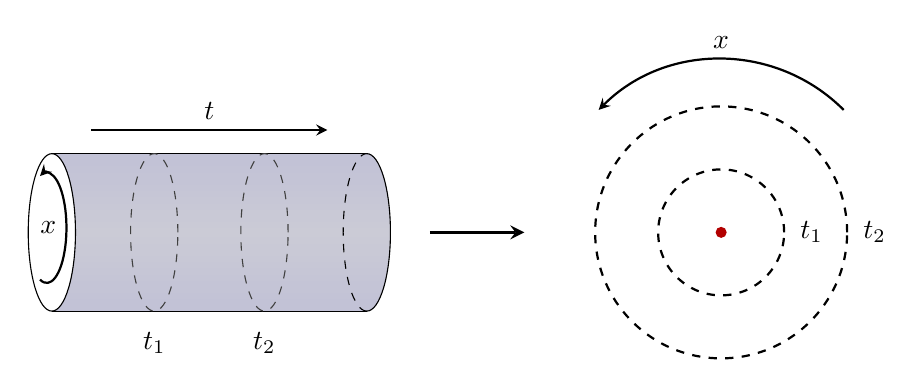
\begin{tikzpicture}[>=stealth]

  % --- 設定 ---
  \def\cylW{4}   % シリンダーの長さ
  \def\cylH{1}   % シリンダーの半径
  \def\persP{0.3} % 遠近感（楕円のつぶれ具合）

  % --- 左側：シリンダーの描画 ---
  % シリンダーの塗りつぶし
  \fill[top color=blue!10, bottom color=blue!10, middle color=blue!5, opacity=0.8]
    (0,\cylH) -- (\cylW,\cylH) arc (90:-90:\persP cm and \cylH cm) -- (0,-\cylH) arc (-90:90:\persP cm and \cylH cm);
  
  % シリンダーの輪郭線
  \draw (0,\cylH) -- (\cylW,\cylH); % 上の線
  \draw (0,-\cylH) -- (\cylW,-\cylH); % 下の線
  \draw (0,0) ellipse (\persP cm and \cylH cm); % 左の面（円）
  \draw (\cylW,\cylH) arc (90:-90:\persP cm and \cylH cm); % 右の面（手前）
  \draw[dashed, thin] (\cylW,-\cylH) arc (-90:-270:\persP cm and \cylH cm); % 右の面（奥・点線）

  % t1, t2 のスライス
  \draw[dashed, darkgray] (1.3,0) ellipse (\persP cm and \cylH cm);
  \draw[dashed, darkgray] (2.7,0) ellipse (\persP cm and \cylH cm);

  % t1, t2 のラベル
  \node at (1.3, -1.4) {$t_1$};
  \node at (2.7, -1.4) {$t_2$};

  % t方向の矢印
  \draw[->, thick] (0.5, 1.3) -- (3.5, 1.3) node[midway, above] {$t$};

  % x方向の矢印
  \draw[->, thick] (-0.15, -0.6) arc (-110:110:0.25cm and 0.7cm) node[midway, left] {$x$};


  % --- 真ん中：写像の矢印 ---
  \draw[->, very thick] (\cylW + 0.8, 0) -- (\cylW + 2.0, 0);


  % --- 右側：平面（動径量子化）の描画 ---
  \begin{scope}[shift={(\cylW + 4.5, 0)}] 
    
    % 原点
    \fill[red!70!black] (0,0) circle (2pt);

    % 同心円
    \draw[dashed, thick] (0,0) circle (0.8cm);
    \draw[dashed, thick] (0,0) circle (1.6cm);

    % t1, t2 のラベル
    \node at (0.8 + 0.35, 0) {$t_1$};
    \node at (1.6 + 0.35, 0) {$t_2$};

    % x方向の矢印
    \draw[->, thick] (45:2.2) arc (45:135:2.2) node[midway, above] {$x$};

  \end{scope}

 \end{tikzpicture}
 \caption{シリンダーから平面への写像（動径量子化）}
 \label{p1}
\end{figure}
この写像において、時間方向$t$は原点からの距離$r$に対応しており、空間方向$x$は角度$\theta$に対応する。
無限の過去$t\rightarrow -\infty$は原点$r\rightarrow 0$に対応し、無限の未来$t\rightarrow \infty$は無限遠$r\rightarrow \infty$に対応する。
このようにして、時間方向と空間方向を対等に扱うことが出来る。
したがって、時間並進演算子$H$は動径方向のスケール変換の生成子に対応する。一方、空間並進演算子$P$は回転の生成子に対応する。
\begin{align}
    H=&L_0 + \overline{L}_0\\
    P=&i(L_0 - \overline{L}_0
    )
\end{align}
\\
場の量子論における時間順序積に対応するものとして動径順序積を以下に定義する。
\begin{align}
    \mathcal{R}\qty(\phi_1(z_1,\overline{z}_1)\phi_2(z_2,\overline{z}_2))=&
    \begin{cases}
    \phi_1(z_1,\overline{z}_1)\phi_2(z_2,\overline{z}_2) & |z_1|>|z_2|\\
    \phi_2(z_2,\overline{z}_2)\phi_1(z_1,\overline{z}_1) & |z_1|<|z_2|
    \end{cases}
\end{align}
OPE(operator product expansion演算子積展開)も同様に動径順序積を用いて定義される。
OPEと交換関係は次のような関係になっている。
\begin{align}
    \oint_{\omega}dz \ a(z)b(\omega)=\oint_{C_1} dz \ a(z)b(\omega)-\oint_{C_2} dz \ b(\omega)a(z)=[A,b(\omega)]\label{p2}
\end{align}
$A$という演算子は$a(z)$を固定した時間で周回積分したものである。つまり
\begin{align}
    A=\oint_{C_1} dz \ a(z)
\end{align}
である。式(\ref{p2})を図で表したものが図\ref{p3}である。

\begin{figure}[htbp]
 \begin{tikzpicture}
  % --- スタイル定義（矢印の修正済み） ---
  \tikzset{midarrow/.style={
      decoration={markings, mark=at position 0.55 with {\arrow{stealth}}},
      postaction={decorate}
    }
  }

  % --- 設定 ---
  \def\Rsmall{0.7}  % 小さい円の半径
  \def\Rbig{2.2}    % 大きい円 C1 の半径
  \def\Rmedium{1.4} % 中くらいの円 C2 の半径
  
  % w の相対位置 (x, y)
  \def\wx{1.5}
  \def\wy{0.8}

  % === 1. 左の図（原点 (0,0) を中心に描画） ===
  \coordinate (O1) at (0,0);
  \coordinate (W1) at (\wx, \wy);

  % 点 0 と w
  \fill[red!70!black] (O1) circle (1.5pt) node[left, black, scale=0.8] {$0$};
  \fill[red!70!black] (W1) circle (1.5pt) node[right, black, scale=0.8] {$w$};
  % w の周りの円
  \draw[midarrow] (W1) circle (\Rsmall);


  % === 等号 (=) ===
  \node at (3.5, 0) {$=$};


  % === 2. 真ん中の図（x=6.5 を中心に描画） ===
  \coordinate (O2) at (6.5, 0);
  \coordinate (W2) at (6.5 + \wx, \wy);

  % 点 0 と w
  \fill[red!70!black] (O2) circle (1.5pt) node[left, black, scale=0.8] {$0$};
  \fill[red!70!black] (W2) circle (1.5pt) node[right, black, scale=0.8] {$w$};
  % 大きな円 C1
  \draw[midarrow] (O2) circle (\Rbig);
  \node at ($(O2) + (225:\Rbig+0.3)$) {$C_1$};


  % === 引き算 (-) ===
  \node at (10.5, 0) {$-$};


  % === 3. 右の図（x=13.0 を中心に描画） ===
  \coordinate (O3) at (13.0, 0);
  \coordinate (W3) at (13.0 + \wx, \wy);

  % 点 0 と w
  \fill[red!70!black] (O3) circle (1.5pt) node[left, black, scale=0.8] {$0$};
  \fill[red!70!black] (W3) circle (1.5pt) node[right, black, scale=0.8] {$w$};
  % 中くらいの円 C2
  \draw[midarrow] (O3) circle (\Rmedium);
  \node at ($(O3) + (225:\Rmedium+0.3)$) {$C_2$};

 \end{tikzpicture}
 \caption{積分経路の変形}
 \label{p3}
\end{figure}
図\ref{p3}では$C_1$を$\omega$よりも大きい円、$C_2$を$\omega$よりも小さい円とした。演算子$B$もAと同様に定義すると、次の交換関係が成り立つことが分かる。
\begin{align}
    [A,B]=&\oint_{0}d\omega[A,b(\omega)]\\
    =&\oint_{0}d\omega \oint_{\omega}dz \ a(z)b(\omega)
\end{align}
\subsubsection{状態と演算子の対応関係}
動径量子化の枠組みにおいて重要な状態演算子対応 (state-operator correspondence) を考える。まず、いかなる場の挿入もなされていない状態を真空状態 $\ket{0}$ と定義する。
このとき、過去の無限遠 ($\tau \to -\infty$) は複素平面上の原点 ($z=0$) に写像されるため、始状態 $\ket{\phi_{\text{in}}}$ は原点への演算子の挿入によって次のように記述される。
\begin{align}
    \ket{\phi_{\text{in}}}=\lim_{z,\overline{z}\rightarrow 0}\phi(z,\overline{z})\ket{0}
\end{align}
同様に終状態$\bra{\phi_{\text{out}}}$も定義したい。
円筒が存在していた空間はミンコフスキー空間であったので、エルミート共役が時空座標に影響を与えることはない。
しかし、複素平面上ではエルミート共役によりユークリッド時間が反転する必要がある。それを確認する。
時間$t$を虚軸に解析接続$it\rightarrow \tau$して得られる空間の時間並進を考える。\footnote{
    このようにユークリッド時間をとったのは計量を正値計量にするためである。
}演算子$A(\tau,x)$はハイゼンベルグ方程式より
\begin{align}
A(\tau,x)=e^{H\tau}A(0,x)e^{-H\tau}    \label{heisen}
\end{align}
が成り立っている。
この関係式のエルミート共役は
\begin{align}
    A(\tau ,x)^\dagger=e^{-H\tau}A(0,x)^\dagger e^{H\tau}
\end{align}
となる。時間並進の後にエルミート共役をとったものは$\tau=0$における演算子を時間反転して推進したものになっていることに注意する。
ハイゼンベルグ方程式を満たすため、ユークリッド空間における共役も\eqref{heisen}式を満たす必要がある。そのためには時間反転を含む必要がある。
この複合変換をユークリッド空間におけるエルミート共役とし、この節では$^+$と書くことにする。
つまり、次の関係式が成り立つ。
\begin{align}
    A(\tau,x)^+=e^{H\tau}A(0,x)^+e^{-H\tau}
\end{align}
以上より、ユークリッド空間におけるエルミート空間は時間の反転に注意して、  $z\rightarrow e^{\frac{2\pi}{l}(-t+ix)}=\frac{1}{z^*}$の変換に対応している。
したがって、プライマリ場$\phi$に対してエルミート共役は次の関係を持っていることが分かる。\footnote{
    この変換は共形変換ではないが、正則な変換$w=1/z$の変換を考え、その結果から変換$w=1/\bar{z}$をエルミート共役の定義としている。
}
\begin{align}
    \phi^\dagger(z,\overline{z})&\equiv\phi'(z,\bar{z})\\
    \phi(1/\overline{z},1/z)&=(\overline{z})^{2h}(z)^{2\bar{h}}\phi'(z,\overline{z})\\
     \phi^\dagger(z,\overline{z})&=(\overline{z})^{-2h}(z)^{-2\bar{h}} \phi(1/\overline{z},1/z)\label{hermite}
\end{align}
out状態のブラベクトルをこのエルミート共役を使って次のように定義する。
\begin{align}
    \bra{\phi_{\text{out}}}=\ket{\phi_{\text{in}}}^\dagger
\end{align}
このとき、内積は次のように計算することが出来る。
\begin{align}
    \braket{\phi_{\text{out}}}{\phi_{\text{in}}}=&\lim_{z,\overline{z}\rightarrow 0}\bra{0}\phi^\dagger(z,\overline{z})\phi(0,0)\ket{0}\\
    =&\lim_{z,\overline{z}\rightarrow 0}\bra{0}(\overline{z})^{-2h}(z)^{-2\bar{h}} \phi(1/\overline{z},1/z)\phi(0,0)\ket{0}\\
    =&\lim_{\xi,\overline{\xi}\rightarrow \infty}\bar{\xi}^{2h}\xi^{2\bar{h}}\bra{0}\phi(\bar{\xi},\xi)\phi(0,0)\ket{0}\label{162}
\end{align}
2点関数の表式\ref{111}を用いると、これは$\xi$に依らない定数になることが分かる。
\\
次に、場のモード展開を考える。ここでは場$\phi(z,\bar{z})$のべき展開をおこなう。
\begin{align}
    \phi(z,\overline{z})=\sum_{m,n}\phi_{m,n}z^{-m-h}\overline{z}^{-n-\overline{h}}\label{phi expansion}
\end{align}
エルミート共役をとると次のようになる。
\begin{align}
    \phi^\dagger(z,\overline{z})=&\sum_{m,n}\phi_{m,n}^\dagger \bar{z}^{-m-h}z^{-n-\overline{h}}\label{168}
\end{align}
ここで、(\ref{162})式より、次のように表示することもできる。
\begin{align}
    \phi^\dagger(z,\overline{z})=&\overline{z}^{-2h}z^{-2\bar{h}}\sum_{m,n}\phi_{m,n}(1/\overline{z})^{-m-h}(1/z)^{-n-\overline{h}}\\
    =&\sum_{m,n}\phi_{m,n}\overline{z}^{m - h} z^{n - \overline{h}}\\
    =&\sum_{m,n}\phi_{-m,-n}z^{-n - \overline{h}}\overline{z}^{-m - h}
\end{align}
つまりこの式と(\ref{168})式を比較すると次の関係式が成り立つことが分かる。
\begin{align}
    \phi_{m,n}^\dagger=\phi_{-m,-n}
\end{align}
\subsubsection{共形変換の生成子とビラソロ代数}
ヒルベルト空間における共形変換の生成子を考える。
共形生成子のカレントは$T_{\mu\nu}\epsilon^{\nu}$という表式を持っていた。
anti-holomorphic部分な部分を無視して、holomorphic部分のみを考える。
このとき、共形変換に対する保存電荷は共形Ward-Takahashiの恒等式(\ref{conformal Ward takahashi})より次のように書ける。
\begin{align}
    Q_{\epsilon}=&\frac{1}{2\pi i}\oint dz \ \epsilon(z) T(z)
\end{align}
これが共形変換の生成子であることを確かめる。エネルギー運動量テンソルとプライマリ場の演算子積展開を用いると次のようになる。
\begin{align}
    [Q_{\epsilon},\phi(w,\overline{w})]=&\frac{1}{2\pi i}\oint_{w} dz \ \epsilon(z) \ev{T(z)\phi(w,\overline{w})}\notag\\
    =&\frac{1}{2\pi i}\oint_{w} dz \ \epsilon(z) \qty(\frac{h}{(z-w)^2}+\frac{1}{z-w}\partial_w)\phi(w,\overline{w})\notag\\
    =&\epsilon(w)\partial_w \phi(w,\overline{w})+h(\partial_w \epsilon(w))\phi(w,\overline{w})\notag\\
    =&-\delta_{\epsilon}\phi(w,\overline{w})\ \ (\because\ (\ref{98}))
\end{align}
したがって、$Q_{\epsilon}$は共形変換の生成子であることが分かる。
\\
次にエネルギー運動量テンソルのモード展開を考える。
\begin{align}
    T(z)=\sum_{n}L_n z^{-n-2}\label{178}
\end{align}
このとき、$L_n$は次のように定義されている。
\begin{align}
    L_n=&\frac{1}{2\pi i}\oint dz \ z^{n+1} T(z)\label{179}
\end{align}
この表式になることを確かめるために(\ref{178})式を(\ref{179})式に代入すると
次のようになる。
\begin{align}
      L_n=&\frac{1}{2\pi i}\oint dz \ z^{n+1} \sum_{m}L_m z^{-m-2}\\
      =&\sum_{m}L_m \frac{1}{2\pi i}\
    \oint dz \ z^{n - m -1}\\
        =&L_n
\end{align}
したがって、$L_n$の表式の十分性が確かめられた。
\\
同様に$\epsilon(z)$のモード展開を考える。
\begin{align}
    \epsilon(z)=&\sum_{n}\epsilon_n z^{n+1}
\end{align}
このとき、共形変換の生成子$Q_{\epsilon}$は次のように書ける。
\begin{align}
    Q_{\epsilon}=&\frac{1}{2\pi i}\oint dz \ \qty(\sum_{n}\epsilon_n z^{n+1})\qty( \sum_{m}L_m z^{-m-2})\\
    =&\sum_{n}\epsilon_n L_n
\end{align}
2つ目の等号はコーシーの積分定理より$-1$乗の項のみが寄与する。
したがって、$L_n$とanti-holomorphic部分の$\overline{L}_n$によりヒルベルト空間における共形変換の生成子を表すが出来る。
\\
$L_n$と$L_m$の交換関係を求める
。\footnote{
    エネルギー運動量テンソル2つの積のOPEは中心電荷cを用いて
       $ T(z)T(\omega)\sim \frac{c/2}{(z-\omega)^4}+\frac{2T(\omega)}{(z-\omega)^2}+\frac{\partial_{\omega}T(\omega)}{z-\omega}$と与えられる。
    詳しい説明は自由ボソンの節を参照。
}
\begin{align}
    [L_n,L_m]=&\frac{1}{(2\pi i)^2}\oint_{0}d\omega \ \omega^{m+1}\oint_{\omega} dz \ z^{n+1} T(z)T(\omega)\notag\\
    =&\frac{1}{(2\pi i)^2}\oint_{0}d\omega \ \omega^{m+1}\oint_{\omega} dz \ z^{n+1} \qty(\frac{c/2}{(z-\omega)^4}+\frac{2T(\omega)}{(z-\omega)^2}+\frac{\partial_{\omega}T(\omega)}{z-\omega}+reg.)\notag\\
    =&\frac{1}{2\pi i}\oint_{0}d\omega \ \omega^{m+1}\qty(\frac{c}{12}(n+1)n(n-1)\omega^{n-2}+2(n+1)\omega^n T(\omega)+\omega^{n+1}\partial_{\omega}T(\omega))\notag\\
    =&\frac{c}{12}n(n^2-1)\delta_{n+m,0} + (n - m) L_{n+m}\label{virasoro algebra}
\end{align}
これらの代数関係をビラソロ代数と呼ぶ。今後$L_n$のことをビラソロ代数の生成子と呼ぶ。
同様にして、anti-holomorphic部分についても次のようなビラソロ代数が成り立つ。
\begin{align}
    [\overline{L}_n,\overline{L}_m]=&\frac{c}{12}n(n^2-1)\delta_{n+m,0} + (n - m) \overline{L}_{n+m}
\end{align}
また、holomorphic部分とanti-holomorphic部分は独立であるため、次の関係式も成り立つ。
\begin{align}
    [L_n,\overline{L}_m]=0
\end{align}
\subsubsection{バーマ加群}
ビラソロ代数の表現としてバーマ加群を考える。
まず、真空状態を
考える。真空状態とは、何も演算子が挿入されていない状態である。
真空状態に対して、エネルギー運動量を考えた時、すなわち$T(z)\ket{0},\overline{T}(\bar{z})\ket{0}$
を考えた時、始状態で特異的な振る舞いを持たないことが要求される。つまり、$z,\bar{z}\rightarrow0$で特異性を持たないために
真空状態に対して次の条件が成り立つ。
\begin{align}
    L_n\ket{0}=&0 \ (n\geq -1) \ \ (\because \ref{178})  \\
    \overline{L}_n\ket{0}=&0 \ (n\geq -1)
\end{align}
漸近状態はプライマリ場の挿入により得られる。
原点におけるプライマリ場$\phi(0,0)$の挿入により得られる始状態$\ket{\phi}$は次のように定義される。
\begin{align}
    \ket{h,\bar{h}}\equiv\phi(0,0
    )\ket{0}
\end{align}
ビラソロ代数の生成子とプライマリ場との交換関係を計算すると次のようになる。
\begin{align}
    [L_n,\phi(z,\overline{z})]=&\frac{1}{2\pi i}\oint_{z}d\omega \ \omega^{n+1} T(\omega)\phi(z,\overline{z})\\
    =&\frac{1}{2\pi i}\oint_{z}d\omega \ \omega^{n+1}\qty(\frac{h}{(\omega - z)^2}+\frac{1}{\omega - z}\partial_z)\phi(z,\overline{z})\ \ (\because\ref{OPE of T and phi })\\
    =&h(n+1)z^n \phi(z,\overline{z})+z^{n+1}\partial_z \phi(z,\overline{z})   \label{commutator of L and phi} 
  \end{align}
    したがって、原点におけるプライマリ場の挿入により得られる始状態に対して次の関係式が成り立つ。
\begin{align}
    L_0\ket{h,\bar{h}}=&(L_0\phi(0,0)-\phi(0,0)L_0)\ket{0}\\
    =&h\ket{h,\bar{h}} \ \ (\because\ref{commutator of L and phi} \text{式の$n=0$の場合})
\end{align}
同様にantiholomorphic部分についても次の関係式が成り立つ。
\begin{align}
    \overline{L}_0\ket{h,\bar{h}}=&\bar{h}\ket{h,\bar{h}}
\end{align}
また、$n>0$の場合についても同様にして次の関係式が成り立つ。
\begin{align}
    L_n\ket{h,\bar{h}}=&0 \ (n>0)\\
    \overline{L}_n\ket{h,\bar{h}}=&0 \ (n>0)
\end{align}
生成子$L_{-n}(n>0)$は共形次元を増加させる作用素である。それを確認する。
\begin{align}
    L_0(L_{-n}\ket{h,\bar{h}})=&(L_{-n}L_0+[L_0,L_{-n}])\ket{h,\bar{h}}\\
    =& (h+n)(L_{-n}\ket{h,\bar{h}})
\end{align}
ここで、\eqref{virasoro algebra}式より
\begin{align}
    [L_0,L_{-n}]=nL_{-n}
\end{align}
が成り立つことを用いた。この式はビラソロ代数の生成子を連続的に作用させることにより、より大きい共形次元の状態を作り出せることを意味している。
これを繰り返すことにより、無限に多くの状態を作り出せる。
このようにして作り出される状態全体の空間をバーマ加群と呼ぶ。
\\
以上の構成法で生成できる状態は一般に次のように表される。
\begin{align}
    L_{\lambda}\ket{h}\equiv L_{-\lambda_1}L_{-\lambda_2}\cdots L_{-\lambda_k}\ket{h}\ \ \ (\lambda=(\lambda_1,\lambda_2,\cdots,\lambda_k),\ \lambda_1\geq \lambda_2\geq \cdots \geq \lambda_k>0)
\end{align}
このとき、増加した共形次元は$N=|\lambda|=\sum_i \lambda_i$である。これをdescendantのレベルと呼び、その状態をディセンダント状態(descendant state)と呼ぶ。
同様にして、anti-holomorphic部分についてもバーマ加群を定義できる。
\begin{align}
    \overline{L}_{\overline{\lambda}}\ket{\bar{h}}\equiv \overline{L}_{-\overline{\lambda}_1}\overline{L}_{-\overline{\lambda}_2}\cdots \overline{L}_{-\overline{\lambda}_l}\ket{\bar{h}}\ \ \ \qty(\overline{\lambda}=(\overline{\lambda}_1,\overline{\lambda}_2,\cdots,\overline{\lambda}_l),\ \overline{\lambda}_1\geq \overline{\lambda}_2\geq \cdots \geq \overline{\lambda}_l>0)
\end{align}
このとき、増加した共形次元は$\overline{N}=|\overline{\lambda}|=\sum_i \overline{\lambda}_i$である。
バーマ加群全体は次のように表される。
\begin{align}
    \mathcal{V}_{h,\bar{h}}=\text{span}\qty{L_{\lambda}\overline{L}_{\overline{\lambda}}\ket{h,\bar{h}}}
\end{align}
これらを用いて、内積を書き換える。まず、次のビラソロ代数の生成子の関係を確認する。
\begin{align}
    (L_n)^\dagger=&L_{-n}\label{209}
\end{align}
これを確認するために、エネルギー運動量テンソルのエルミート共役を考える。
\begin{align}
    T^\dagger(z,\overline{z})=&\sum_{n}L_n^\dagger \overline{z}^{-n-2}\notag
\end{align}
一方、(\ref{hermite})式より\footnote{
    エネルギー運動量テンソルとは共形次元が(2,0)の準プライマリ場であることに注意する。この共形次元を持つことはエネルギー運動量テンソル同士のOPEを計算すれば分かる。
}
\begin{align}
    =&(\overline{z})^{-4}\sum_{n}L_{-n} (1/\overline{z})^{-n-2}\notag\\
    =&(\overline{z})^{-4}\sum_{n}L_{-n} \overline{z}^{n+2}\notag\\
    =&\sum_{n}L_{-n} \overline{z}^{-n-2}
\end{align}
従って(\ref{209})式が成り立つことが分かる。
\\これを用いて、双対ベクトルに対して次が成り立つことが分かる。
\begin{align}
    \bra{h}L_j=0 \ (j>0)\\
\end{align}
2つの状態$L_{\mu}\ket{h}$と$L_{\lambda}\ket{h}$の内積を考える。
\begin{align}
    \bra{h}L_{\mu}^\dagger L_{\lambda}\ket{h}=&\bra{h}L_{-\mu_k}\cdots L_{-\mu_2}L_{-\mu_1}L_{-\lambda_1}L_{-\lambda_2}\cdots L_{-\lambda_l}\ket{h}\\
    =&\bra{h}L_{\mu_k}\cdots L_{\mu_2}L_{\mu_1}L_{-\lambda_1}L_{-\lambda_2}\cdots L_{-\lambda_l}\ket{h}
\end{align}
このようにして、内積は最終的に$\bra{h}L_{-n}L_n\ket{h}$の形に帰着される。
これはビラソロ代数の交換関係(\ref{virasoro algebra})式を用いることにより評価することが出来る。
\\

ユニタリな表現を考えるとき、内積が正定値であることが要求される。
この条件を満たすためには、共形次元$h,\bar{h}$と中心電荷$c$に制限が課される。
$L_{-1}\ket{\psi}$のノルムを計算する。
\begin{align}
    |L_{-1}\ket{\psi}|^2=\bra{\psi}L_1 L_{-1}\ket{\psi}=&\bra{\psi}[L_1,L_{-1}]\ket{\psi}\notag\\
    =&2h \braket{\psi}
\end{align}
これが0以上であるためには$h\geq 0$である必要がある。
\\
次に$L_{-n}\ket{0}$のノルムを計算する。
\begin{align}
    |L_{-n}\ket{0}|^2=\bra{0}L_n L_{-n}\ket{0}=&\bra{0}[L_n,L_{-n}]\ket{0}\notag\\
    =&\frac{c}{12}n(n^2-1) \braket{0}
\end{align}
ここで、$c=0$とすると、全てのビラソロ代数の生成子が真空を消滅させてしい、励起状態が存在しない自明な理論になる。
したがって、非自明なCFTにおいては中心電荷は$c>0$である必要がある。
\subsubsection{ディセンダント場}
プライマリ状態はプライマリ場を挿入して得られたものであった。
一方、ディセンダント状態に関しても同様にして対応する場がどのような表式になっているのかを確認する。
例として、$L_{-n}\ket{h}(n>0)$に対応する場を考える。
このディセンダント状態はビラソロ代数の生成子の定義より次のように書き換えることが出来る。
\begin{align}
    L_{-n}\ket{h}=&\lim_{w \rightarrow 0}\frac{1}{2\pi i}\oint dz \ z^{-n+1} T(z)\phi(w)\ket{0}\\
    =&\lim_{w\rightarrow 0}\frac{1}{2\pi i}\oint dz \ z^{-n+1} T(z)\phi(w)\ket{0}
\end{align}
今までは、OPEとして、二つの座標が近づく極限において発散する部分のみを取り出して考えていた。
しかし、この場合は被積分項$z^{-n+1}$もあるので、有限部分も残す必要があり、OPEを次のように展開する。
\begin{align}
    T(z)\phi(w)=\frac{\phi^{(0)}(w)}{(z-w)^2}+\frac{\phi^{(-1)}(w)}{z-w}+\phi^{(-2)}(w)(z-w)^0+\phi^{(-3)}(w)(z-w)^1+\cdots
\end{align}
このとき、ディセンダント状態は次のように書くことが出来る。
\begin{align}
    L_{-n}\ket{h}=&\lim_{w\rightarrow 0}\frac{1}{2\pi i}\oint dz \ z^{-n+1}\qty(\frac{\phi^{(0)}(w)}{(z-w)^2}+\frac{\phi^{(-1)}(w)}{z-w}+\phi^{(-2)}(w)(z-w)^0+\cdots)\ket{0}\notag\\
    =&\lim_{w\rightarrow 0}\frac{1}{2\pi i}\oint dz \ z^{-n+1}\qty(\sum_{k=0}^{\infty}\phi^{(-k)}(w)(z-w)^{
    k-2})\ket{0}\notag\\
    =&\lim_{w\rightarrow 0}\sum_{k=0}^{\infty}\qty(\frac{1}{2\pi i}\oint dz \ z^{-n+1}(z-w)^{k-2})\phi^{(-k)}(w)\ket{0}\notag\\
    =&\lim_{w\rightarrow 0}\sum_{k=0}^{\infty}\qty(\frac{1}{2\pi i}\oint dz \ (z-w+w)^{-n+1}(z-w)^{k-2})\phi^{(-k)}(w)\ket{0}\notag\\
      =&\lim_{w\rightarrow 0}\phi^{(-n )}(w)\ket{0}
\end{align}
$w\rightarrow 0$より$w$のべき乗は残らないことに注意する。
したがって、ディセンダント状態$L_{-n}\ket{h}$はディセンダント場
\begin{align}
    \phi^{(-n)}(w)=\frac{1}{2\pi i}\oint dz \ (z-w)^{-n+1}T(z)\phi(w)\label{descendant field}
\end{align}
を原点に挿入することにより得られる。
$\phi$がプライマリ場であることに注意すると\eqref{OPE of T and phi }式より次の関係が成り立っている。
\begin{align}
    \phi^{(0)}(w)=&h\phi(w)\\
    \phi^{(-1)}(w)=&\partial_w \phi(w)
\end{align}
重要な例として$\phi$が恒等場$\bm{1}$で考える。\eqref{descendant field}式を用いて
\begin{align}
    \bm{1}^{(-2)}(w)=\frac{1}{2\pi i}\oint dz \ T(z)\frac{1}{z-w}=\ T(w)
\end{align}
となる。したがって、エネルギー運動量テンソル$T(z)$は恒等場のレベル2のディセンダント場である。
\\

一般のディセンダント場も構成することが出来る。
ディセンダント状態$L_{-m}L_{-n}\ket{h}$に対してはディセンダント場$\phi^{(-m,-n)}$を次のように定義する。
\begin{align}
    \phi^{(-m,-n)}(w)=\frac{1}{2\pi i} \oint dz (z-w)^{-m+1}T(z)\phi^{(-n)}(w)
\end{align}
より一般のディセンダント場も同様にして定義できる。
\begin{align}
    L_{-k_1}\cdots L_{-k_j}\ket{h}=&\lim_{w\rightarrow 0}\phi^{(-k_1,\cdots,-k_j)}(w)\ket{0}\leftrightarrow \phi^{(-k_1,\cdots,-k_j)}(w)\notag\\&\hspace{4cm}
    =\frac{1}{2\pi i}\oint dz \ (z-w)^{-k_1+1}T(z)\phi^{(-k_2,\cdots,-k_j)}(w)
\end{align}
この様にして構成される場の全体を共形族と呼び、$[\phi]$のように記述することにする。
\\
ここまではプライマリ場の相関関数について考えてきたが、これからはディセンダント場$\phi^{(-k)}(w)$を1つ含むような相関関数について考える。
ディセンダント場を1つ含む相関関数は
\begin{align}
    \ev{\phi^{(-k)}(w)\phi_1(z_1,\overline{z}_1)\cdots \phi_n(z_n,\overline{z}_n)}=&\frac{1}{2\pi i}\oint_w dz \ (z-w)^{-k+1}\ev{T(z)\phi(w)\phi_1(z_1,\overline{z}_1)\cdots \phi_n(z_n,\overline{z}_n)}
\end{align}
と書ける。ここで、
積分路は$z=w$のみを含み、他の点$z_j$を含まないように選ぶ。この積分路を変形して、$w$を含まず、その他の各座標
$z_j$をとり囲んだ積分路の和にする。
\begin{align}
    \ev{\phi^{(-k)}(w)\phi_1(z_1,\overline{z}_1)\cdots \phi_n(z_n,\overline{z}_n)}=&-\sum_{j=1}^{n}\frac{1}{2\pi i}\oint_{z_j} dz \ (z-w)^{-k+1}\ev{T(z)\phi(w)\phi_1(z_1,\overline{z}_1)\cdots \phi_n(z_n,\overline{z}_n)}
\end{align}
ここで$T(z)$と$\phi_j(z_j)$とのOPEを用いて次のように書き換える。
\begin{align}
    \ev{\phi^{(-k)}(w)\phi_1(z_1,\overline{z}_1)\cdots \phi_n(z_n,\overline{z}_n)}=&-\sum_{j=1}^{n}\frac{1}{2\pi i}\oint_{z_j} dz \ (z-z_j+z_j-w)^{-k+1}\qty(\frac{h_j}{(z-z_j)^2}+\frac{1}{z-z_j}\partial_{z_j})\nonumber\\
    &\times \ev{\phi(w)\phi_1(z_1,\overline{z}_1)\cdots \phi_n(z_n,\overline{z}_n)}\notag\\
    =&\sum_{j=1}^n\frac{1}{2\pi i} \oint_{z_j} dz \ \qty(\frac{(k-1)h_j}{(z-z_j)(z_j-w)^k}-\frac{1}{(z-w)^{k-1}(z_i-z_j)}\partial_{z_j})\nonumber\\
    &\times \ev{\phi(w)\phi_1(z_1,\overline{z}_1)\cdots \phi_n(z_n,\overline{z}_n)}\nonumber \\
    &\hspace{10mm} \qty(\because\text{二項定理} \binom{-k+1}{m}=(-1)^m\binom{k-1+m}{m})\notag\\
    =&\sum_{j=1}^{n}\qty(\frac{(k-1)h_j}{(z_j - w)^k} - \frac{1}{(z_j - w)^{k-1}}\partial_{z_j})\ev{\phi(w)\phi_1(z_1,\overline{z}_1)\cdots \phi_n(z_n,\overline{z}_n)}\label{descendant eq}
\end{align}
ここで微分演算子$\mathcal{L}_{-k}$を次のように定義する。
\begin{align}
    \mathcal{L}_{-k}^{(w)}\equiv \sum_{j=1}^{n}\qty(\frac{(k-1)h_j}{(z_j - w)^k} - \frac{1}{(z_j - w)^{k-1}}\partial_{z_j})
\end{align}
このとき、ディセンダント場を1つ含む相関関数は次のように書ける。
\begin{align}
    \ev{\phi^{(-k)}(w)\phi_1(z_1,\overline{z}_1)\cdots \phi_n(z_n,\overline{z}_n)}=&\mathcal{L}_{-k}^{(w)}\ev{\phi(w)\phi_1(z_1,\overline{z}_1)\cdots \phi_n(z_n,\overline{z}_n)}
\end{align}
\section{自由ボソンと自由フェルミオン}
ここでは、自由ボソンと自由フェルミオンについて考える。
\subsection{場の量子論}
\subsubsection{2点関数の計算}
場の量子論の準備をする。
相関関数の定義から、2点関数は次のように記述される。ユークリッド空間で考えていることに注意する。
\begin{align}
    \ev{\mathcal{T}(\phi(x_1)\phi(x_2))}=&\frac{\int \mathcal{D}\phi \ \phi(x_1)\phi(x_2)e^{-S[\phi]}}{\int \mathcal{D}\phi \ e^{-S[\phi]}}\label{2point}
\end{align}
この2点関数の他の表式を確認する。そのために次の生成汎関数を定義する。
\begin{align}
    Z[J]=&\int \mathcal{D}\phi \ e^{-S[\phi]+\int d^dx \ J(x)\phi(x)}\label{generating}
\end{align}
$J(x)$は外部ソースである。この生成汎関数を用いると、2点関数は次のように書ける。
\begin{align}
    \ev{\mathcal{T}(\phi(x_1)\phi(x_2))}=&\frac{1}{Z[0]}\qty(\frac{\delta}{\delta J(x_1)})\qty(\frac{\delta}{\delta J(x_2)})Z[J]\Bigg|_{J=0}
\end{align}
2点関数を計算するために、作用積分として次のような表式を仮定する。
\begin{align}
    S[\phi]=&\int d^dx d^dy \ \qty(\frac{1}{2}\phi(x)A(x,y)\phi(y) )\label{234}
\end{align}
$A$は$x,y$の関数である。
このときの経路積分\eqref{generating}式のの中の指数関数の中身は次のように書ける。
\begin{align}
    -S[\phi]+\int d^dx \ J(x)\phi(x)=&\frac{-1}{2}\int d^dx d^dy \ \phi(x)A(x,y)\phi(y) + \int d^dx \ J(x)\phi(x)
\end{align}
$\phi\rightarrow\phi+\phi_0$という変数変換を考える。このとき、積分測度は不変である。
\begin{align}
    &\frac{-1}{2}\int d^dx d^dy \ \qty(\phi(x)+\phi_0(x))A(x,y)\qty(\phi(y)+\phi_0(y)) + \int d^dx \ J(x)\qty(\phi(x)+\phi_0(x))\\
    =&\frac{-1}{2}\int d^dx d^dy \ \phi(x)A(x,y)\phi(y) + \int d^dx \ \qty(-\int d^dy \ A(x,y)\phi_0(y) + J(x))\phi(x)\\
    &+\frac{-1}{2}\int d^dx d^dy \ \phi_0(x)A(x,y)\phi_0(y) + \int d^dx \ J(x)\phi_0(x)\nonumber
\end{align}
ここで、$\phi_0$を次のように選ぶ。この選び方は上の式の2項目の括弧の中を0にするように決める。
\begin{align}
    -\int d^dy \ A(x,y)\phi_0(y) + J(x)=0\ \rightarrow \phi_0(x)=\int d^dy \ A^{-1}(x,y)J(y)
\end{align}
このとき、生成汎関数の指数部分は
\begin{align}
    -S[\phi]+\int d^dx \ J(x)\phi(x)=&\frac{-1}{2}\int d^dx d^dy \ \phi(x)A(x,y)\phi(y) \notag\\
    &+\frac{-1}{2}\int d^dx d^dy \ \phi_0(x)A(x,y)\phi_0(y) + \int d^dx \ J(x)\phi_0(x)\nonumber
    \\
    =&\frac{-1}{2}\int d^dx d^dy \ \phi(x)A(x,y)\phi(y) 
    +\frac{1}{2}\int d^dx d^dy \ J(x)A^{-1}(x,y)J(y)
\end{align}
と書ける。
(\ref{2point})式により、次のように2点関数が書ける。
\begin{align}
    \ev{\mathcal{T}(\phi(x_1)\phi(x_2))}=&A^{-1}(x_1,x_2)
\end{align}
\subsubsection{自由ボソンにおける2点関数}
2次元において質量のない自由ボソン場の作用は次のように与えられる。
\begin{align}
    S[\phi]=&\frac{1}{8\pi}\int d^2x \ \partial_{\mu}\phi \partial^{\mu}\phi\label{free boson}
\end{align}
このとき(\ref{234})式と見比べ部分積分をすることにより、関数$A(x,y)$
は次の表式で与えられる。
\begin{align}
    A(x,y)=&-\frac{1}{4\pi}\square\delta^{(2)} (x-y)
\end{align}
部分積分をして、境界項を無視した。$\delta^{(2)}(x-y)=\delta(x_1-y_1)\delta(x_2-y_2)$に注意する。\\
このとき、2点関数を$K(x,y)$とすると
次の式が成り立つ。
\begin{align}
    \int d^2z \ A(x,z)K(z,y)=&\delta(x-y)\\
    -\frac{1}{4\pi}\int d^2z \ \square\delta^{(2)}(x-z) K(z,y)=&\delta^{(2)}(x-y)\\
-\frac{1}{4\pi}\partial^2 K(x,y)=&\delta^{(2)}(x-y)
\end{align}
つまり、2点関数はこの方程式のグリーン関数であることが分かる。
\\
点$y$を中心とする半径$R$の円の領域で積分すると
次のように変形される。
\begin{align}
     -\frac{1}{4\pi}\int_D d^2x \ \partial^2 K(x,y)=&\int_D d^2x \ \delta(x-y)\\
\end{align}
$K(x,y)\equiv K(\rho),\rho=|x-y|$としてガウスの発散定理を用いると次のようになる。
\begin{align}
    -\frac{1}{4\pi}\oint_{\partial D} ds \ \hat{n}\cdot \nabla K(\rho)=&1
\end{align}
ここで、$\hat{n}$は境界に垂直な単位ベクトルである。
また、$ds=R d\theta$である。
したがって、次のようになる。
\begin{align}
    -\frac{1}{4\pi}\int_0^{2\pi}R d\theta \ \partial_{\rho} K(\rho)\Big|_{\rho=R}=&1\\
   R \partial_{\rho} K(\rho)\Big|_{\rho=R}=&-2
\end{align}
したがって、次のように2点関数が求まる。
\begin{align}
    K(R)=&-2\ln R + \text{const.} \\
    \ev{\phi(x)\phi(y)}=&- \ln |x-y|^2 + \text{const.}
\end{align}
つまり、自由ボソン場の2点関数の表式が求まった。
\subsection{Wickの定理}
前節では2点関数について扱っていたが、ここでは一般の$n$点関数について考える。
そのために、Wickの定理を紹介する。
\\

場の量子論では、自由場の場の演算子を生成演算子と消滅演算子に分解する。
\begin{align}
    \phi(x)=\phi^{+}(x)+\phi^{-}(x)
\end{align}
$\phi^{+}(x)$が生成演算子であり、$\phi^{-}(x)$が消滅演算子である。
消滅演算子は真空状態$\ket{0}$に作用すると0になる。
\\次に、正規順序を定義する。
正規順序とは、生成演算子を左側に、消滅演算子を右側に並べる操作である。
例えば、2つの場の正規順序は次のように定義される。
\begin{align}
    :\phi(x_1)\phi(x_2):=&\phi^{+}(x_1)\phi^{+}(x_2)+\phi^{+}(x_1)\phi^{-}(x_2)+\phi^{+}(x_2)\phi^{-}(x_1)+\phi^{-}(x_1)\phi^{-}(x_2)
\end{align}
$::$で挟まれた部分は正規順序をとっていることを示している。
正規順序を使って、時間順序積が次のように表せる。
ここでは$x^0_1>x^0_2$の場合を考える。
\begin{align}
    \mathcal{T}(\phi(x_1)\phi(x_2))=&:\phi(x_1)\phi(x_2):+[\phi(x_1)^- ,\phi(x_2)^+]
\end{align}
この真空期待値をとると、正規順序の部分は0になることから、交換子の部分を次のように変形できることが分かる。
\begin{align}
   \mathcal{T}(\phi(x_1)\phi(x_2))=&:\phi(x_1)\phi(x_2):+\ev{\phi(x_1)\phi(x_2)}
\end{align}
2点関数の部分を次のように簡約する。
\begin{align}
    \ev{\phi(x_1)\phi(x_2)}\equiv \contraction{}{\phi}{(x_1)}{\phi}\phi(x_1)\phi(x_2)
\end{align}
Wickの定理は異なる点の時間順序積に対して、
正規順序にすべての可能な簡約を足し合わせたものとして表せることを述べている。
例えば、4点関数の場合、Wickの定理を用いて
\begin{align}
    \mathcal{T}\phi(x_1)\phi(x_2)\phi(x_3)\phi(x_4)=&:\phi(x_1)\phi(x_2)\phi(x_3)\phi(x_4):\notag\\
    &+:\contraction{}{\phi}{(x_1)}{\phi}\phi(x_1)\phi(x_2):\phi(x_3)\phi(x_4):+\contraction{}{\phi}{(x_1)\phi(x_2)\phi(x_3)}{\phi}\phi(x_1)\phi(x_2)\phi(x_3)\phi(x_4):\notag\\
    &+:\contraction{\phi(x_1)}{\phi}{(x_2)}{\phi}\phi(x_1)\phi(x_2)\phi(x_3)\phi(x_4):+\contraction{\phi(x_2)}{\phi}{(x_2)\phi(x_3)}{\phi}\phi(x_1)\phi(x_2)\phi(x_3)\phi(x_4) +\contraction{\phi(x_1)\phi(x_2)}{\phi}{(x_3)}{\phi}\phi(x_1)\phi(x_2)\phi(x_3)\phi(x_4)\notag\\
    & +:\contraction{}{\phi}{(x_1)\phi(x_2)}{\phi}\contraction[2ex]{\phi(x_1)}{\phi}{(x_2)\phi(x_3)}{\phi}\phi(x_1)\phi(x_2)\phi(x_3)\phi(x_4):\notag\\
    &+:\contraction{}{\phi}{(x_1)}{\phi}\contraction[2ex]{\phi(x_1)\phi(x_2)}{\phi}{(x_3)}{\phi}\phi(x_1)\phi(x_2)\phi(x_3)\phi(x_4):
    +:\contraction{}{\phi}{(x_1)\phi(x_2)\phi(x_3)}{\phi}\contraction[2ex]{\phi(x_1)}{\phi}{(x_2)}{\phi}\phi(x_1)\phi(x_2)\phi(x_3)\phi(x_4):
\end{align}
と表される。
\subsection{自由ボソンにおける演算子積展開}
ここでは質量のない自由ボソン場に対して、演算子積展開を考える。
まず、作用の表式\eqref{free boson}式より、変分原理から運動方程式を記述すると次のようになる。
\begin{align}
    \square \phi(x)=0
\end{align}
これを複素座標で書き直すと次のようになる。\footnote{
$\partial_z=\frac{1}{2}(\partial_1 - i \partial_2)$, $\partial_{\overline{z}}=\frac{1}{2}(\partial_1 + i \partial_2)$であったことに注意する。
}
\begin{align}
    \partial_z \partial_{\overline{z}}\phi(z,\overline{z})=0
\end{align}
これが意味することは、$\partial_z \phi(z,\overline{z})$は$\overline{z}$に依存しない関数であり、$\partial_{\overline{z}} \phi(z,\overline{z})$は$z$に依存しない関数であるということである。
次にエネルギー運動量テンソルを考える。(\ref{energy momentum tensor})式より次のように与えられる。
\begin{align}
    T_{\mu\nu}=&-\eta_{\mu\nu}\qty(\frac{1}{8\pi}\partial_{\alpha}\phi \partial^{\alpha}\phi) + \frac{1}{4\pi}\partial_{\mu}\phi \partial_{\nu}\phi\\
    =&\frac{1}{4\pi}\qty(\partial_{\mu}\phi \partial_{\nu}\phi - \frac{1}{2}\eta_{\mu\nu}\partial_{\alpha}\phi \partial^{\alpha}\phi)
\end{align}
これは対称でトレースレスなテンソルになっている。複素座標で書き換えると$-\frac{1}{2\pi}T=T_{zz}, T_{zz}=\frac{1}{4}(T_{00}-2iT_{01}-T_{11})$
という関係を用いて次のようになる。\footnote{
    エネルギー運動量テンソルがトレースレスより、$T_{00}+T_{11}=0$に注意する。
}
\begin{align}
    T(z)=&-2\pi T_{zz}=-2\pi(2T_{00}-2iT_{01})\\
    =&\frac{1}{8}(\partial_0\phi-i\partial_1\phi)^2=-\frac{1}{2}\qty(\partial_z \phi(z)\partial_z \phi(z))\\
=&- \frac{1}{2}:\partial_z \phi(z)\partial_z \phi(z):\label{boson energy momentum tensor}
\end{align}
2つ目の等号はエネルギー運動量テンソルの真空期待値を0にするために正規順序をとっていることに注意する。反正則部分についても同様にして次のように書ける。
これにしたがって、2点関数は複素座標を用いて次のように表される。
\begin{align}
    \ev{\phi(z,\overline{z})\phi(w,\overline{w})}=&- \ln |z-w|^2= - \ln (z-w) - \ln (\overline{z}-\overline{w})+\text{const}
\end{align}
この表式から分かる通り、自由ボソン場$\phi$はプライマリ場ではない。
しかし、$\partial \phi$はプライマリ場である。これを確認する。
正則な部分に特に注目して、議論を進める。$\partial_z, \partial_w$の微分をとると次のようになる。
\begin{align}
    \ev{\partial_z \phi(z)\partial_w \phi(w)}=&-\frac{1}{(z-w)^2}
\end{align}
従って、$\partial \phi$のOPEは次のように与えられる。
\begin{align}
    \partial_z \phi(z)\partial_w \phi(w)\sim& -\frac{1}{(z-w)^2} 
\end{align}
ここで、$\sim$は等式ではなく、特異性のみを示していることに注意する。
\\
$T(z)$と$\partial \phi$のOPEを計算する。
\begin{align}
    T(z)\partial_w \phi(w)=&-\frac{1}{2}:\partial_z \phi(z)\partial_z \phi(z):\partial_w \phi(w)\\
    \sim& -\frac{1}{2}\qty(\contraction{\partial_z\phi(z)}{\partial_z}{\phi(z)}{\partial_z}\partial_z \phi(z)\partial_z \phi(z)\partial_w \phi(w) + \contraction{}{\partial_z}{\phi(z)\partial_z \phi(z)}{\partial_w}\partial_z \phi(z)\partial_z \phi(z)\partial_w \phi(w))\\
    \sim& \frac{1}{(z-w)^2}\partial_z \phi(z) 
\end{align}
$\partial \phi(z)$を$w$の周りで展開すると、次のようになる。
\begin{align}
   T(z)\partial_w \phi(w)\sim& \frac{1}{(z-w)^2}\partial_w \phi(w) + \frac{1}{(z-w)}\partial_w^2 \phi(w) \\
\end{align}
これを(\ref{OPE of T and phi })式と見比べることにより$\partial \phi(z)$は共形次元が1のプライマリ場であることが分かる。
Wickの定理により、エネルギー運動量テンソル同士のOPEも計算できる。
\begin{align}
    T(z)T(w)=&\frac{1}{4}:\partial_z \phi(z)\partial_z \phi(z): :\partial_w \phi(w)\partial_w \phi(w):\\
    \sim& \frac{1}{4}\qty(2\contraction{}{\partial_z}{\phi(z)\partial_z\phi(z)}{\partial_w}\contraction[2ex]{\partial_z\phi(z)}{\partial_z}{\phi(z)\partial_w\phi(w)}{\partial_w}\partial_z \phi(z)\partial_z \phi(z)\partial_w \phi(w)\partial_w \phi(w) + 4\contraction{}{\partial_z}{\phi(z)\partial_z \phi(z)}{\partial_w}\partial_z \phi(z)\partial_z \phi(z)\partial_w \phi(w)\partial_w \phi(w))\\
    \sim& \frac{1}{2}\frac{1}{(z-w)^4} + \frac{2}{(z-w)^2}T(w) + \frac{1}{(z-w)}\partial_w T(w)
\end{align}
一般の二次元共形場理論において、エネルギー運動量テンソル同士のOPEは次のように与えられる。
\begin{align}
    T(z)T(w)\sim& \frac{c/2}{(z-w)^4} + \frac{2}{(z-w)^2}T(w) + \frac{1}{(z-w)}\partial_w T(w)\label{OPE of T and T}
\end{align}
ここで、$c$は中心電荷と呼ばれており、理論の自由度を表している。
N個の自由ボソン場の系では、中心電荷は$c=N$となり、N個のフェルミオン場の系では$c=N/2$となる。これは次の節で詳しく説明する。
一般の理論ではエネルギー運動量テンソルは準プライマリ場であるが、プライマリ場ではない重要な例となっている。\footnote{
    エネルギー運動量テンソルが共形次元(2,0)の場であるため、$(z-w)^2,(z-w)$の項の係数はエネルギー運動量テンソルと準プライマリ場のOPEより決定することが出来る。更にこのOPEに
        $\frac{\mathcal{A}_n(w)}{(z-w)^n} \ \ \ (n\geq 3)$
    の項を加えることが出来る。この形の共形次元は、エネルギー運動量テンソルが(2,0)であることより、(4,0)でなければならない。したがって、$\mathcal{A}_n(w)$は共形次元が$(4-n,0)$でなければならない。この論文では詳細を示さないが、ユニタリな理論では共形ウェイトが非負でなければならない。したがって、$n=3,4$のみが適する。
ここで、$T(z)$がボーズ統計性を持つため、
$    T(z)T(w)    =T(w)T(z)$
を満たす。これを用いると、$\mathcal{A}_4(w)$は定数であり、$\mathcal{A}_3(w)$は0であることが分かる。
    したがって、エネルギー運動量テンソル同士のOPEは(\ref{OPE of T and T})式の形になることが分かる。
}
\\

エネルギー運動量テンソルがプライマリ場でないことを確かめる。
共形Ward-Takahashiの恒等式(\ref{conformal Ward takahashi})式を用いると次のようになる。
\begin{align}
    \delta_{\epsilon,\overline{\epsilon}} T(w)=&\frac{1}{2\pi i}\oint_{w} dz \ \epsilon(z) T(z)T(w)\\
    =&\frac{1}{2\pi i}\oint_{w} dz \ \epsilon(z)\qty(\frac{c/2}{(z-w)^4} + \frac{2}{(z-w)^2}T(w) + \frac{1}{(z-w)}\partial_w T(w))\\
    =&\frac{c}{12}\partial_w^3 \epsilon(w) + 2 \partial_w \epsilon(w) T(w) + \epsilon(w)\partial_w T(w)\label{infty energy momentum}
\end{align}
(\ref{98})式と比べると、3次の微分項が余分に存在していることが分かる。
したがって、エネルギー運動量テンソルはプライマリ場ではない。大域的な共形変換に対しては、$\epsilon$が高々2次の多項式であるため、この余分な項は消える。
\\
有限変換$z\rightarrow w(z)$に対するエネルギー運動量テンソルの変換則は
\begin{align}
    \widetilde{T}(w)=&\qty(\frac{dw}{dz})^{-2}\qty[T(z) - \frac{c}{12}S(w,z)]\label{energy momentum trans}
\end{align}
と書ける。
ここで、$S(w,z)$はシュワルツ微分と呼ばれるものであり、次のように定義される。
\begin{align}
    S(w,z)=&\frac{d^3 w/dz^3}{dw/dz} - \frac{3}{2}\qty(\frac{d^2 w/dz^2}{dw/dz})^2
\end{align}
ここではこの有限変換の無限小変換が先ほどの表式と合う事と、この有限変換が群構造をなしていることを確かめてみる。
まず、無限小変換を考える。$w=z+\epsilon(z)$とする。
\begin{align}
    \frac{dw}{dz}=&1+\partial_z \epsilon(z)\\
    \qty(\frac{dw}{dz})^{-2}=&1 - 2\partial_z \epsilon(z)\\
    S(w,z)=& \partial_z^3 \epsilon(z)-\frac{3}{2}(\partial_z^2 \epsilon(z))^2
\end{align}
これを(\ref{energy momentum trans})式に代入すると次のようになる。
\begin{align}
    \widetilde{T}(w)=&\qty(1 - 2\partial_z \epsilon(z))\qty[T(z) - \frac{c}{12}\qty(\partial_z^3 \epsilon(z)-\frac{3}{2}(\partial_z^2 \epsilon(z))^2)]\\
    =&T(z) - 2\partial_z \epsilon(z) T(z) - \frac{c}{12}\partial_z^3 \epsilon(z) + \mathcal{O}(\epsilon^2)
\end{align}
したがって、(\ref{infty energy momentum})の表式と合うことが分かる。
\\

次に群構造が成り立つことを確かめる。
2回の変換$z\rightarrow w(z)\rightarrow v(w)$を考える。
$z$での微分を$'$で$w$での微分を$\dot{}$で表す。
\begin{align}
    \widetilde{T}(w)=&\qty(w')^{-2}\qty[T(z) - \frac{c}{12}S(w,z)]\\
    \widetilde{T}(v)=&\qty(\dot{v})^{-2}\qty[\widetilde{T}(w) - \frac{c}{12}S(v,w)]\notag\\
    =&\qty(\dot{v})^{-2}\qty[\qty(w')^{-2}\qty[T(z) - \frac{c}{12}S(w,z)] - \frac{c}{12}S(v,w)]\notag\\
    =&\qty(\frac{dv}{dz})^{-2}\qty[T(z) - \frac{c}{12}\qty(S(w,z) + (w')^2 S(v,w))]
\end{align}
ここで、微分に関して
\begin{align}
   v'=& \dot{v} w'\\
   v''=& \ddot{v}(w')^2 + \dot{v} w''\\
   v'''=& \dddot{v}(w')^3 + 3\ddot{v} w' w'' + \dot{v} w'''
\end{align}
が成り立つので、シュワルツ微分について次の関係式が成り立つ。
\begin{align}
    S(v,z)=& \frac{v'''}{v'} - \frac{3}{2}\qty(\frac{v''}{v'})^2\\
    =&\frac{ \dddot{v}(w')^3 + 3\ddot{v} w' w'' + \dot{v} w'''}{\dot{v} w'}-\frac{3}{2}\qty(\frac{\ddot{v}(w')^2 + \dot{v} w''}{\dot{v} w'})^2\\
    =& (w')^2 \qty(\frac{\dddot{v}}{\dot{v}} - \frac{3}{2}\qty(\frac{\ddot{v}}{\dot{v}})^2) + S(w,z)\\
    =& (w')^2 S(v,w) + S(w,z)
\end{align}
この関係式を用いることにより、エネルギー運動量テンソルの変換は次のように書ける。
\begin{align}
    \widetilde{T}(v)=&\qty(\frac{dv}{dz})^{-2}\qty[T(z) - \frac{c}{12}S(v,z)]
\end{align}
したがって、群構造であることが確かめられた。したがって、\eqref{energy momentum trans}が成り立つ。
\subsection{自由ボソン}
\subsubsection{モード展開}
ここでは自由ボソンのモード展開を考える。
まず、ミンコフスキー空間において円筒上に定義された自由ボソン場$\varphi$を考える。
今一度、作用積分を与える。
\begin{align*}
    S[\varphi]=&\frac{1}{8\pi}\int d^2x \ \partial_{\mu}\varphi \partial^{\mu}\varphi
\end{align*}
$\varphi$が円筒上で定義されているという事は次の周期的境界条件を満たす。
\begin{align}
    \varphi(x+l,t)=&\varphi(x,t)
\end{align}
変分原理により、場$\varphi$の運動方程式は次のようになる。
\begin{align}
    \partial_{\mu}\partial^{\mu}\varphi=[\partial_t^2 - \partial_x^2]\varphi=0
\end{align}
この2つの条件を満たす一般解として、次のようなモード展開が与えられる。
\begin{align}
    \varphi_{\text{cyc}}=&=\varphi_0+\frac{4\pi}{l}\pi_0 t+i\sum_{n\neq 0}\frac{1}{n}\qty(a_n e^{-i\frac{2\pi}{l}n(t-x)} + \overline{a}_n e^{-i\frac{2\pi}{l}n(t+x)})
\end{align}
周期性があるのは形から明らかである。運動方程式を満たすのか確認する。
\begin{align}
    [\partial_t^2 - \partial_x^2]\varphi_{\text{cyc}}=&i\sum_{n\neq 0}\frac{1}{n}\qty(a_n \qty(-i\frac{2\pi}{l}n)^2 e^{-i\frac{2\pi}{l}n(t-x)} + \overline{a}_n \qty(-i\frac{2\pi}{l}n)^2 e^{-i\frac{2\pi}{l}n(t+x)} )\nonumber\\
    &-i\sum_{n\neq 0}\frac{1}{n}\qty(a_n \qty(i\frac{2\pi}{l}n)^2 e^{-i\frac{2\pi}{l}n(t-x)} + \overline{a}_n \qty(i\frac{2\pi}{l}n)^2 e^{-i\frac{2\pi}{l}n(t+x)} )\nonumber\\
    =&0
\end{align}
共役な運動量は次の表式になっている。
\begin{align}
    \Pi_{\text{cyc}}(x,t)=&\frac{\delta S}{\delta (\partial_t \varphi_{\text{cyc}})}=\frac{1}{4\pi}\partial_t \varphi_{\text{cyc}}
\end{align}
場の量子論ではこれらの場と場に共役な運動量に対して次の同時刻交換関係を課す。
\begin{align}
    [\varphi_{\text{cyc}}(x,t),\Pi_{\text{cyc}}(y,t)]=&i\delta(x-y)\label{commutation relation} \\
    [\varphi_{\text{cyc}}(x,t),\varphi_{\text{cyc}}(y,t)]=&0\label{commutation relation 2}\\
    [\Pi_{\text{cyc}}(x,t),\Pi_{\text{cyc}}(y,t)]=&0\label{commutation relation 3}
\end{align}
特に(\ref{commutation relation})式に場のモード展開を代入すると次のようになる。
\begin{align}
    &\Bigg[\varphi_0+\frac{4\pi}{l}\pi_0 t+i\sum_{n\neq 0}\frac{1}{n}\qty(a_n e^{-i\frac{2\pi}{l}n(t-x)} + \overline{a}_n e^{-i\frac{2\pi}{l}n(t+x)})\\
    &\ \ \ \ \ \ , \frac{1}{4\pi}\qty(\frac{4\pi}{l}\pi_0 + \sum_{m\neq 0}\qty(\frac{2\pi}{l}a_m e^{-i\frac{2\pi}{l}m(t-y)}  +\frac{2\pi }{l}\overline{a}_m e^{-i\frac{2\pi}{l}m(t+y)}))\Bigg]\nonumber
    =i\delta(x-y)
\end{align}
この式を逆フーリエ変換して、各モードの交換関係を求めると次のようになる。
つまり、$x$で積分すればよい。
\begin{align}
    &\int_0^l dx \ e^{i\frac{2\pi}{l}p x}\Bigg[\varphi_0+\frac{4\pi}{l}\pi_0 t+i\sum_{n\neq 0}\frac{1}{n}\qty(a_n e^{-i\frac{2\pi}{l}n(t-x)} + \overline{a}_n e^{-i\frac{2\pi}{l}n(t+x)})\\
    &\ \ \ \ \ \ , \frac{1}{4\pi}\qty(\frac{4\pi}{l}\pi_0 + \sum_{m\neq 0}\qty(\frac{2\pi}{l}a_m e^{-i\frac{2\pi}{l}m(t-y)}  +\frac{2\pi }{l}\overline{a}_m e^{-i\frac{2\pi}{l}m(t+y)}))\Bigg]\nonumber
    =i\int_0^l dx \ e^{i\frac{2\pi}{l}p x}\delta(x-y)\nonumber
\end{align}
$p=0$のとき、指数の部分が消えるので、次のようになる。
\begin{align}
    [\varphi_0 , \pi_0]=&i
\end{align}
次に振動項を見るために、$p\neq 0$のときを考える。
\begin{align}
    &\int_0^l dx \ e^{i\frac{2\pi}{l}p x}\Bigg[i\sum_{n\neq 0}\frac{1}{n}\qty(a_n e^{-i\frac{2\pi}{l}n(t-x)} + \overline{a}_n e^{-i\frac{2\pi}{l}n(t+x)}) , \frac{1}{4\pi}\sum_{m\neq 0}\qty(\frac{2\pi}{l}a_m e^{-i\frac{2\pi}{l}m(t-y)}  +\frac{2\pi }{l}\overline{a}_m e^{-i\frac{2\pi}{l}m(t+y)})\Bigg]\nonumber\\
    =&i\int_0^l dx \ e^{i\frac{2\pi}{l}p x}\delta(x-y)\\
    &\int_0^l dx \ e^{i\frac{2\pi}{l}p x}\Bigg[i\sum_{n\neq 0}\frac{1}{n} a_n e^{-i\frac{2\pi}{l}n(t-x)} ,\frac{2\pi}{l} \frac{1}{4\pi}\sum_{m\neq 0} a_m e^{-i\frac{2\pi}{l}m(t-y)}\Bigg]\nonumber\\
    &+\int_0^l dx \ e^{i\frac{2\pi}{l}p x}\Bigg[i\sum_{n\neq 0}\frac{1}{n} \overline{a}_n e^{-i\frac{2\pi}{l}n(t+x)} , \frac{2\pi}{l}\frac{1}{4\pi}\sum_{m\neq 0} \overline{a}_m e^{-i\frac{2\pi}{l}m(t+y)}\Bigg]\nonumber\\
    =&i e^{i\frac{2\pi}{l}p y}
\end{align}
$a$について$[a_n,\bar{a}_m]=0$とした。
更に、$n,m$についての和を外に出すと次のようになる。
\begin{align}
    &i\sum_{n\neq 0}\sum_{m\neq 0}\frac{2\pi}{l}\frac{1}{4\pi n}\int_0^l dx \ e^{i\frac{2\pi}{l}p x}\qty(e^{-i\frac{2\pi}{l}(n x + m y)}[ a_n , a_m] + e^{-i\frac{2\pi}{l}(-n x + m y)}[ \overline{a}_n , \overline{a}_m])\\
    =&i e^{i\frac{2\pi}{l}p y}
\end{align}
積分の中で１項目が有効であるのは$n=p$のときである。このとき、右辺と等しくなるためには$m=-p$となる
必要がある。一方、2項目が有効となるのは$n=-p$の時である。このとき、右辺と等しくなるためには$m=p$となる必要がある。同様に\eqref{commutation relation 2}\eqref{commutation relation 3}も考えて次のようになる。
\begin{align}
[a_n , a_m]=& n \delta_{n+m,0}\\
[\overline{a}_n , \overline{a}_m]=& n \delta_{n+m,0}
\\
[a_n , \overline{a}_m]=& 0
\end{align}
自由ボソンに対するハミルトニアンは次のようになる。
\begin{align}
    H=\int d^dx (\Pi \partial_t \varphi) - L=&\frac{1}{8\pi}\int_0^l dx \ \qty((\partial_t \varphi_{\text{cyc}})^2 + (\partial_x \varphi_{\text{cyc}})^2) \\
    =&\frac{1}{8\pi}\int_0^l dx[:(\partial_t \varphi_{\text{cyc}})^2: + :(\partial_x \varphi_{\text{cyc}})^2: ]
\end{align}
最後の行はハミルトニアンの真空期待値を0として、正規順序をとっている。
モード展開を代入して計算すると次のようになる。
\begin{align}
    H=&\frac{2\pi}{l}\qty(\pi_0^2 + \frac{1}{4}\sum_{n>0} (a_{-n} a_n + a_n a_{-n} + \overline{a}_{-n} \overline{a}_n + \overline{a}_n \overline{a}_{-n}))\\
    =&\frac{2\pi}{l}\qty(\pi_0^2 + \frac{1}{2}\sum_{n>0} (:a_{-n} a_n: + :\overline{a}_{-n} \overline{a}_n:))\label{hamiltonian}
\end{align}
エネルギー固有値が有限となるよう、無限の定数項を無視し正規順序をとっている。正規順序の中身が$a_{-n}a_m$の順になっているが、$a_{-n}(n>0)$が生成演算子として、機能することを確認する。
$a_{-n}$が生成演算子であることは、交換関係から次のように確認できる。
\begin{align}
    [H,a_{-n}]=&\frac{2\pi}{l}\qty([ \sum_{m>0} :a_{-m} a_m: , a_{-n}])\\
    =&\frac{2\pi}{l}na_{-n}
\end{align}
これは$a_{-n}$が生成演算子であることを表しており、例えばエネルギー固有値$E$のエネルギー固有状態$\ket{E}$に対して、$\hat{H}\hat{a}_{-n}\ket{E}$という状態を考えてみると
、$(E+2n\pi/l)a_{-n}\ket{E}$となっていることが分かる。
同様にして、$a_n (n>0)$は消滅演算子として機能する。
\subsubsection{円筒と平面の関係}
これまではミンコフスキー空間上の円筒について議論してきたが、これ以降複素平面を用いるため、ユークリッド空間に移って議論する。
そのために$t$を虚時間$\tau$に変換する。
\begin{align}
    it\rightarrow& \tau
\end{align}
次に$w=\tau-ix,\overline{w}=\tau+ix$と定義する。
$w$は複素変数であり、$\overline{w}$はその共役複素数である。
ここで、ボソン場のモード展開を再度書き下す。
\begin{align}
    \varphi_{\text{cyl}}(w,\overline{w})=&\varphi_0 - i\frac{2\pi}{l}\pi_0 (w+\overline{w}) + i\sum_{n\neq 0}\frac{1}{n}\qty(a_n e^{-\frac{2\pi}{l}n w} + \overline{a}_n e^{-\frac{2\pi}{l}n \overline{w}})
\end{align}
$w\sim w+l $という同一視をしている。
次に、円筒から平面への
\begin{align}
    z=e^{\frac{2\pi}{l}w},\overline{z}=e^{\frac{2\pi}{l}\overline{w}}
\end{align}
という写像を考える。この写像により、$w\sim w+l$という同一視は$z\sim e^{2\pi}z$という同一視に変換される。
この同一視を取り除くために、$z$平面上で$0<|z|<\infty$の領域を考える。
平面上の自由ボソン場は単に$w\rightarrow z$への置き換えで次のように与えられる。
\begin{align}
    \varphi_{\text{plane}}(z,\overline{z})\int&\varphi_0 - i\frac{2\pi}{l}\pi_0 \frac{l}{2\pi}(\ln z + \ln \overline{z}) + i\sum_{n\neq 0}\frac{1}{n}\qty(a_n z^n + \overline{a}_n \overline{z}^n)\\
    =&\varphi_0 - i \pi_0 \ln |z|^2 + i\sum_{n\neq 0}\frac{1}{n}\qty(a_n z^{-n} + \overline{a}_n \overline{z}^{-n})
\end{align}
正則な部分にのみ注目し、$\partial \varphi$というものに注目する。
\begin{align}
    \partial_z \varphi(z)=&-i \frac{\pi_0}{z} - i\sum_{n\neq 0} a_n  z^{-n-1}\\
    i\partial_z\varphi(z)=& \sum_{n=-\infty}^{\infty} a_n
    z^{-n-1}
\end{align}
ここで$a_0\equiv \overline{a}_0\equiv \pi_0$とした。
ここで、(\ref{phi expansion})式と比較すると、$\partial \varphi$は$h=1$のプライマリ場であることが分かる。\footnote{
    これを結論づけるためには$\phi_{m,n}^\dagger=\phi_{-m,-n}$が成り立っていたのと同様に$a_n^\dagger=a_{-n}$が成り立ってていて欲しい。
        実際に、$\varphi^\dagger$が$\varphi(z,\overline{z})$と等しいためには、$a_n^\dagger=a_{-n},\overline{a}_n^\dagger=\overline{a}_{-n}$が成り立つ必要がある。
}
モード展開を用いて、2点関数を計算する。$a_n(n\geq0)$が真空状態に作用すると0になることに注意する。%%なぜ0の時は入れないのか分からない。
\begin{align}
    \ev{\varphi(z)\partial_w\varphi(w)}=& \sum_{n,m\neq 0}\frac{1}{n}\ev{a_n a_m} z^{-n} w^{-m-1}
    \end{align}
生成消滅演算子の交換関係を用いて、次のようになる。
\begin{align}
    \ev{\varphi(z)\partial_w\varphi(w)}=& \sum_{n,m>0}\frac{1}{n} \ev{a_{n}a_{-m}} z^{-n} w^{m-1}\notag\\
    =&\sum_{n>0}\frac{1}{n} n z^{-n} w^{n-1}\notag\\
    =& \sum_{n>0} (w/z)^{n} \frac{1}{w}\notag\\
    =& \frac{1}{w}\frac{w/z}{1 - w/z}\notag\\
    =& \frac{1}{z-w}
\end{align}
これを微分すると次のようになる。
\begin{align}
    \ev{\partial_z \varphi(z)\partial_w\varphi(w)}=& -\frac{1}{(z-w)^2}
\end{align}
エネルギー運動量テンソルは(\ref{energy momentum tensor})式より次のようになる。
\begin{align}
    T(z)=&- \frac{1}{2}:\partial_z \varphi(z)\partial_z \varphi(z):\notag\\
    =& -\frac{1}{2}\sum_{m,n}:a_m a_n: z^{-m-n-2}
\end{align}
これはビラソロ代数の生成子が$T(z)=\sum z^{-n-2}L_n$という関係式から、次の表式で与えらえれることを意味している。\footnote{
    holomorphicのエネルギー運動量テンソルは生成演算子での表式における$m+n$を$k$と置くと、$-\frac{1}{2}\sum_{k}\sum_{m}:a_m a_{k-m}: z^{-k-2}=\sum_{n} z^{-n-2}L_n$から$L_n= -\frac{1}{2}\sum_{m}:a_{n-m} a_m:$と導出できる。
}
\begin{align}
L_n=& -\frac{1}{2}\sum_{m}:a_{n-m} a_m:\\
L_0=& \sum_{m>0} a_{-m} a_m + \frac{1}{2} a_0^2
\end{align}
したがって、ハミルトニアン(\ref{hamiltonian})式はビラソロ代数の生成子を用いて次のように表すことが出来る。
\begin{align}
    H=&\frac{2\pi}{l}(L_0 + \overline{L}_0)
\end{align}
この式から分かることは、円周$l$の円筒上に自由ボソンを配置したときのエネルギー固有値はビラソロ代数の生成子$L_0,\overline{L}_0$の固有値によって決定され、
$\frac{2\pi}{l}$に比例しているということである。つまり、円筒上の自由ボソンを調べるにあたって、複素平面に移りビラソロ代数の生成子を用いて円筒上のことについて議論することが出来ると分かる。
これが共形場理論における円筒-平面対応である。
\\

定義より、エネルギー運動量テンソルの真空期待値は$\ev{T(z)}=0$である。
ここまでくると正規順序の定義が希薄になっているが
、これからは演算子積展開から特異項を除くことにより正規順序を定義する。
実際、エネルギー運動量テンソルの真空期待値は次のように表すことが出来る。
\begin{align}
    T(z)=&\lim_{\epsilon \to 0}\qty[-\frac{1}{2}\qty(\partial_z \varphi(z)\partial_z \varphi(z+\epsilon) + \frac{1}{\epsilon^2})]\\
\therefore \ev{T(z)}=&\lim_{\epsilon \to 0}\qty[-\frac{1}{2}\qty(\ev{\partial_z \varphi(z)\partial_z \varphi(z+\epsilon)} + \frac{1}{\epsilon^2})]
\end{align}
この様に平面上でエネルギー運動量テンソルが0になるように理論を組み立てた時、有限の長さ$l$を持つ円周上ではどのように定義されるのかを見ていく。
逆の変数変換$z\rightarrow w=\frac{l}{2\pi}\ln z$を使って(\ref{energy momentum trans})式に従って
エネルギー運動量テンソルの変換を考える。
\begin{align}
    T_{\text{cyl}}(w)=&\qty(\frac{dz}{dw})^{2}\qty[T_{\text{plane}}(z) + \frac{1}{12}S(z,w)]\\
    =&\qty(\frac{2\pi}{l}z)^{2}\qty[T_{\text{plane}}(z)  + \frac{1}{12}\qty(-\frac{1}{2}\frac{1}{z^2})]\\
\end{align}
ここで1個の自由ボソンの中心電荷が$c=1$であることを用いた。
これに対して真空期待値をとると次のようになる。
\begin{align}
    \ev{T_{\text{cyl}}(w)}=&\qty(\frac{2\pi}{l}z)^{2}\qty[\ev{T_{\text{plane}}(z)}  - \frac{1}{24}\frac{1}{z^2}]\\
    =& - \frac{\pi^2}{6 l^2}
\end{align}
これは円筒上におけるビラソロ代数の生成子が次の表式をとることを示唆している。
\begin{align}
    L_{0,\text{cyl}}=& \frac{1}{2}a_0^2 + \sum_{n>0} a_{-n} a_n - \frac{1}{24}
\end{align}
この表式もOPEから真空期待値を引いて、正規順序をとることにより導出する。
    ビラソロ代数の生成子は円筒上で
    \begin{align}
        L_{0,\text{cyl}}=& \oint \frac{dw}{2\pi i} \qty(\frac{dz}{dw})^{-1} z T_{\text{cyl}}(w)\notag\\
        =& \oint \frac{dw}{2\pi i} \qty(\frac{l}{2\pi}\frac{1}{z}) z \qty(\frac{2\pi}{l}z)^{2}\qty[T_{\text{plane}}(z) + \frac{1}{12}S(z,w)]\notag\\
        =& \oint \frac{dz}{2\pi i} z T_{\text{plane}}(z) + \oint \frac{dz}{2\pi i} z \frac{1}{12}\qty(-\frac{1}{2}\frac{1}{z^2})\notag\\
        =& L_{0,\text{plane}} - \frac{1}{24}
        \end{align}
        という表式をとる。
これによりハミルトニアンは次のように表される。
\begin{align}
    H=&\frac{2\pi}{l}(L_{0,\text{cyl}} + \overline{L}_{0,\text{cyl}})\\
    =&\frac{2\pi}{l}\qty(L_{0,\text{plane}}+ \overline{L}_{0,\text{plane}} - \frac{1}{12})
\end{align}
このように、有限の長さ$l$を持つ円周上に自由ボソンを配置したとき、ハミルトニアンには真空エネルギーとして
$-\frac{2\pi}{l}\frac{1}{12}$だけずれることが分かる。これを有限サイズ効果と呼び、より一般には中心電荷$c$を持つ共形場理論に対しては
\begin{align}
    H=&\frac{2\pi}{l}\qty(L_{0,\text{plane}}+ \overline{L}_{0,\text{plane}} - \frac{c}{12})
\end{align}
だけずれることが分かる。
\subsection{自由フェルミオン}
\subsubsection{自由フェルミオンのOPE}
フェルミオン場$\Psi$に対して、次の作用積分を考える。
\begin{align}
    S=&\frac{1}{4\pi}\int d^2x \ \Psi^\dagger \gamma^0 \gamma^{\mu} \partial_{\mu} \Psi
\end{align}
ここで$\gamma^\mu$とはクリフォード代数と呼ばれる行列であり、次の反交換関係を満たしている。
\begin{align}
    \{\gamma^\mu , \gamma^\nu\}=& 2 \eta^{\mu\nu}
\end{align}
ユークリッド空間で、ガンマ行列としてカイラル表示を採用する。
つまり、ガンマ行列の表式を次のように取る。
\begin{align}
    \gamma^0=& \begin{pmatrix}
      0 & 1 \\
      1 & 0
    \end{pmatrix},\ \
    \gamma^1= \begin{pmatrix}
      0 & -i \\
      i & 0
    \end{pmatrix}
\end{align}
このとき、作用は次のように書き換えることが出来る。
\begin{align}
    S=&\frac{1}{4\pi}\int d^2x \ \begin{pmatrix}
        \psi &\bar{\psi}
    \end{pmatrix}\partial_0\begin{pmatrix}
        \psi \\
        \bar{\psi}
    \end{pmatrix}+\begin{pmatrix}
        \psi &\bar{\psi}
    \end{pmatrix}\begin{pmatrix}
      0 & 1 \\
      1 & 0
    \end{pmatrix} \begin{pmatrix}
      0 & -i \\
      i & 0
    \end{pmatrix}
\partial_1\begin{pmatrix}
        \psi \\
        \bar{\psi}
    \end{pmatrix}
    \\
    =&\frac{1}{4\pi}\int d^2x \ \psi\partial_0 \psi + \bar{\psi}\partial_0 \bar{\psi} + i\psi \partial_1 \psi - i\bar{\psi}\partial_1 \bar{\psi}\\
    =&\frac{1}{2\pi}\int d^2x \ (\psi\bar{\partial} \psi + \bar{\psi}\partial\bar{\psi})
\end{align}
運動方程式から$\partial \bar{\psi}=0,\bar{\partial}\psi=0$が得られる。
したがって、$\psi(z)$は正則、$\bar{\psi}(\bar{z})$は反正則な場であることが分かる。
\\

2点関数を計算する。
フェルミオン場の2点関数を次のように置く。
\begin{align}
    K_{i j}=\ev{\Psi_i(x)\Psi_j(x)}
\end{align}
自由ボソン場に対して解析した時の処方箋と同様に求めていく。
自由フェルミオン場に対して作用が
\begin{align}
    S=\frac{1}{2}\int d^2x d^2y \ \Psi_i(x) A_{i j}(x,y) \Psi_j(y)
\end{align}
と書けるとする。この表式を自由フェルミオン場の作用に当てはめてみると、$A_{ij}$は次の表式になることが分かる。
\begin{align}
    A_{i j}(x,y)=&\frac{1}{2\pi} \partial_\mu\delta(x-y) (\gamma^0\gamma^\mu) 
\end{align}
2点関数$K_{ij}$はこれの逆行列になっていることがbosonの場合と同様に示される。
\begin{align}
    \int d^2y \ A_{i k}(x,y) K_{k j}(y,z)=& \delta(x-z)\delta_{i j}\\
    \int d^2y \ \frac{1}{2\pi}\partial_\mu\delta(x-y) (\gamma^0\gamma^\mu)_{ik} K_{k j}(y,z)=& \delta(x-z)\delta_{i j}\\
    \frac{1}{2\pi}\partial_\mu (\gamma^0\gamma^\mu)_{ik} K_{k j}(x,z)=& \delta(x-z)\delta_{i j}\label{free fermion 2point}
\end{align}
これを複素座標を用いて書き直す。\\

そのための準備として、まず$\delta$関数の複素座標表示を考える。
2次元のグリーンの定理より次が成り立つ。
\begin{align}
    \oint f dx +fi dy=& \iint_D \qty(i\pdv{f}{x} -\pdv{f}{y}) dx\wedge dy
\end{align}   
この式に$1/2i$を掛け、複素座標を用いて書くと次のようになる。
\begin{align}
\frac{1}{2i}\int f dz=\int \bar{\partial} f dx\wedge dy
\end{align}
$f=1/z$を採用することにより$\delta$関数の複素座標表示は次のようになる。
\begin{align}
    \delta (z,\bar{z})=& \frac{1}{\pi }\bar{\partial} \qty(\frac{1}{z})=\frac{1}{\pi}\partial\qty(\frac{1}{\bar{z}})\label{deltacom}
\end{align}
これを用いることにより、(\ref{free fermion 2point})式は次のように書き直すことが出来る。
\begin{align}
    \frac{1}{2\pi}\begin{pmatrix}
        \partial_0 & 0 \\
        0& \partial_0
    \end{pmatrix}\begin{pmatrix}
        \ev{\psi(z,\bar{z})\psi(w,\bar{w})} & \ev{\psi(z,\bar{z})\bar{\psi}(w,\bar{w})} \\
        \ev{\bar{\psi}(z,\bar{z})\psi(w,\bar{w})} & \ev{\bar{\psi}(z,\bar{z})\bar{\psi}(w,\bar{w})}
    \end{pmatrix}\nonumber\\+\frac{1}{2\pi}\begin{pmatrix}
         i\partial_1&0 \\
        0 & -i\partial_1
    \end{pmatrix}&\begin{pmatrix}
        \ev{\psi(z,\bar{z})\psi(w,\bar{w})} & \ev{\psi(z,\bar{z})\bar{\psi}(w,\bar{w})} \\
        \ev{\bar{\psi}(z,\bar{z})\psi(w,\bar{w})} & \ev{\bar{\psi}(z,\bar{z})\bar{\psi}(w,\bar{w})}
    \end{pmatrix}\nonumber
    \\=& \begin{pmatrix}
        \delta(z-w,\bar{z}-\bar{w}) & 0 \\
        0 & \delta(z-w,\bar{z}-\bar{w})\end{pmatrix}\\
\frac{1}{\pi}\begin{pmatrix}
    \bar{\partial}&0 \\
      0 & \partial
    \end{pmatrix}\begin{pmatrix}
        \ev{\psi(z,\bar{z})\psi(w,\bar{w})} & \ev{\psi(z,\bar{z})\bar{\psi}(w,\bar{w})} \\
        \ev{\bar{\psi}(z,\bar{z})\psi(w,\bar{w})} & \ev{\bar{\psi}(z,\bar{z})\bar{\psi}(w,\bar{w})}\end{pmatrix}=&\frac{1}{\pi} \begin{pmatrix}
          \bar{\partial}\frac{1}{z-w} & 0 \\
        0  & \partial\frac{1}{\bar{z}-\bar{w}}
        \end{pmatrix}
\end{align}
このとき、2点関数は次のように与えられる。
\begin{align}
    \ev{\psi(z,\bar{z})\psi(w,\bar{w})}=& \frac{1}{z-w}\label{fermion 2point}\\
    \ev{\bar{\psi}(z,\bar{z})\bar{\psi}(w,\bar{w})}=& \frac{1}{\bar{z}-\bar{w}}\\
    \ev{\psi(z,\bar{z})\bar{\psi}(w,\bar{w})}=& 0
\end{align}
holomorphicな場のOPEは次のようになる。
\begin{align}
    \psi(z)\psi(w)\sim\  \frac{1}{z-w} 
\end{align}
フェルミオン場がプライマリ場か否かを調べるためにエネルギー運動量テンソルのOPEを計算する。
エネルギー運動量テンソルは$T^{\mu\nu}_C=-\eta^{\mu\nu}\mathcal{L}+\frac{\partial \mathcal{L}}{\partial (\partial_\mu \Phi)}\partial^\nu \Phi$により、複素座標において次のように計算される。
\begin{align}
    T_{zz}=T_{z}^\lambda g_{\lambda z}=&2T^{\bar{z}}_{z}\notag\\
    =&2\frac{\partial \mathcal{L}}{\partial(\bar{\partial} \psi)}\partial_z \psi\notag\\
    =&\frac{1}{\pi}\psi\partial \psi
\end{align}
以下同様にして次のように計算することが出来る。
\begin{align}
    T_{\bar{z}\bar{z}}=&2\frac{\partial \mathcal{L}}{\partial (\bar{\partial}\Phi)}\partial\Phi=\frac{1}{\pi}\bar{\psi} \bar{\partial} \bar{\psi}\\
    T_{z\bar{z}}=&2\frac{\partial \mathcal{L}}{\partial (\partial\Phi)}\partial\Phi -2\mathcal{L}=-\frac{1}{\pi}\psi \bar{\partial}\psi
\end{align}
このとき、$T^{z\bar{z}},T^{\bar{z}z}$は運動方程式より0になる。
したがって、holomorphicなエネルギー運動量テンソルを$T^{\bar{z}\bar{z}}=-2\pi T(z)$という風に書き換えると、$T(z)$
は次のようになる。
\begin{align}
    T(z)=& -\frac{1}{2}:\psi(z)\partial \psi(z):
\end{align}
有限となるように正規順序を取っている。
この表式はボソンの場合とは異なることに注意する。ここで出てくる正規順序は、フェルミオンの場合反交換関係を用いてOPEから特異項を引くことにより正規順序を定義する。
\begin{align}
    :\psi(z)\partial \psi(z):=& \lim_{\epsilon \to 0}\qty(\psi(z)\partial \psi(z+\epsilon) - \ev{\psi(z)\partial \psi(z+\epsilon)})
\end{align}
フェルミオン場の共形次元を確認するため、次にエネルギー運動量テンソルとフェルミオン場のOPEを計算する。Wickの定理と\eqref{fermion 2point}式より計算することが出来る。
\begin{align}
    T(z)\psi(w)&=-\frac{1}{2}:\psi(z)\partial \psi(z):\psi(w)\notag\\
    &\sim -\frac{1}{2}\contraction{}{\psi(z)}{\partial\psi(z)}{\psi(w)}\psi(z)\partial \psi(z)\psi(w) -\frac{1}{2}\contraction {\psi(z)}{\partial \psi (z)}{}{\psi(w)} \psi(z)\partial \psi(z)\psi(w)\notag\\
    &= \frac{1}{2}\frac{1}{z-w}\partial \psi(z)-\frac{1}{2}\psi(z)\frac{-1}{(z-w)^2}\notag\\
    &\sim \frac{1}{2}\frac{\psi(w)}{(z-w)^2} + \frac{1}{z-w}\partial \psi(w)
\end{align}
したがって、一般のプライマリ場とエネルギー運動量テンソルとのOPEの形\eqref{OPE of T and phi }と一致し、その共形次元は$h=\frac{1}{2}$であることが分かる。
\\

次に中心電荷を求めるため、エネルギー運動量テンソル同士のOPEを計算する。場の交換は反可換であることに注意する。
\begin{align}
    T(z)T(w)&=\frac{1}{4}:\psi(z)\partial \psi(z)::\psi(w)\partial \psi(w):\notag\\
    &\sim \frac{1}{4}\contraction{}{\psi(z)}{\partial \psi(z)\psi(w)}{\partial\psi(w)}\contraction[2ex]{\psi(z)}{\partial \psi(z)}{}{\psi(w)} \psi(z)\partial \psi(z)\psi(w)\partial \psi(w) + \frac{1}{4}\contraction{}{\psi(z)}{\partial \psi(z)}{\psi(w)}\contraction[2ex]{\psi(z)}{\partial \psi(z)}{\psi(w)}{\partial \psi(w)}\psi(z)\partial \psi(z)\psi(w)\partial \psi(w)\nonumber
    +\frac{1}{4}\contraction{}{\psi(z)}{\partial \psi(z)}{\psi(w)}\psi(z)\partial \psi(z)\psi(w)\partial \psi(w)\notag\\  &\ \ \ + \frac{1}{4}\contraction{}{\partial \psi(z)}{\partial \psi(z)\psi(z)}{\partial\psi(w)}\psi(z)\partial \psi(z)\psi(w)\partial \psi(w)+\frac{1}{4}\contraction{\psi(z)}{\partial\psi(z)}{}{\psi(w)}\psi(z)\partial\psi(z)\psi(w)\partial\psi(w)+\frac{1}{4}\contraction{\psi(z)}{\partial\psi(z)}{\psi(w)}{\partial\psi(w)}\psi(z)\partial\psi(z)\psi(w)\partial\psi(w)\notag\\
    &= \frac{1}{4}\frac{1}{(z-w)^2}\frac{-1}{(z-w)^2} - \frac{1}{4}\frac{1}{z-w}\frac{-2}{(z-w)^3} - \frac{1}{4}\frac{1}{z-w}\partial \psi(z)\partial \psi(w) \nonumber\\
    &\ + \frac{1}{4}\frac{1}{(z-w)^2}\psi(z)\partial \psi(w)
    +\frac{1}{4}\frac{-1}{(z-w)^2}\psi(z)\partial\psi(w)-\frac{1}{4}\frac{-2}{(z-w)^3}\psi(z)\psi(w)\notag\\
    &\sim \frac{1/4}{(z-w)^4}+\frac{1}{(z-w)^2}2T(w) + \frac{1}{z-w}\partial T(w)
\end{align}
したがって、プライマリ場の運動量テンソル同士のOPEの形\eqref{OPE of T and T}と一致し、中心電荷は$c=\frac{1}{2}$であることが分かる。
\\

以上より、自由フェルミオン場は共形次元$h=\frac{1}{2}$、中心電荷$c=\frac{1}{2}$の共形場理論を構成することが分かる。
\subsubsection{円筒-平面対応}
自由フェルミオン場を円筒上に配置したときの有限サイズ効果を調べる。
円筒上の座標を$w=t_E - i x$とし、$x$は周期$l$を持つものとする。ここで$t_E$はユークリッド時間であることに注意する。
2つの種類の境界条件を課す。
\begin{align}
    \psi(x+l)=& +\psi(x) \ \ \ \text{Ramond(R)}\\
    \psi(x+l)=& -\psi(x) \ \ \ \text{Neveu-Schwarz(NS)}
\end{align}
円筒上でのフェルミオン場の展開は次のようにして行う。
\begin{align}
    \psi(w)=& \sqrt{\frac{2\pi}{l}}\sum_{k\in \mathbb{Z}+\nu}  b_ke^{-\frac{2\pi}{l} k w}
\end{align}
展開の係数は後で平面上のフェルミオン場の展開係数と合わせるためにこのように取っている。ここで$\nu=0$のときR境界条件、$\nu=\frac{1}{2}$のときNS境界条件である。
フェルミオン場の理論では、正準反交換関係は次のようになる。
\begin{align}
    \{\psi(x),\psi(y)\}=&  2\pi\delta(x-y)
\end{align}
これを用いると、展開係数に対して次の反交換関係が成り立つ。
\begin{align}
    \qty{\sqrt{\frac{2\pi}{l}}b_ke^{-\frac{2\pi}{l} k (t-ix)} , \sqrt{\frac{2\pi}{l}}b_{k'}e^{-\frac{2\pi}{l} k' (t-iy)}}=& \frac{2\pi}{l} e^{i\frac{2\pi}{l}k(x-y)}\\
    \qty{b_k , b_{k'}}=&  \delta_{k+k',0}
\end{align}
後に、ハミルトニアンとの交換関係を調べたら明らかになることであるが、$k>0$のとき$b_k$は消滅演算子、$k<0$のとき$b_k$は生成演算子として働く。
Ｒ境界条件の場合、$k$は整数値をとるため、$k=0$のモードが存在し、このモードは真空の縮退を誘発する演算子として働く。
平面上の座標$z$との関係は次のようになる。
\begin{align}
    z=& e^{\frac{2\pi}{l}w}
\end{align}
自由ボソンの場合と異なり、フェルミオン場は共形次元が$\frac{1}{2}$であるため、次のように変換される。
\begin{align}
    \psi_{\text{plane}}(z)=&\qty(\frac{dz}{dw})^{-\frac{1}{2}}\psi_{\text{cyl}}(w)\\
    =&\qty(\frac{l}{2\pi z})^{\frac{1}{2}}\psi_{\text{cyl}}(w)
\end{align}
したがって、平面上のフェルミオン場は次のように展開される。
\begin{align}
    \psi_{\text{plane}}(z)=& \sqrt{\frac{2\pi}{l}}\sum_{k\in \mathbb{Z}+\nu} b_k \qty(\frac{2\pi}{l})^{-\frac{1}{2}} z^{-k-\frac{1}{2}}\\
    =& \sum_{k\in \mathbb{Z}+\nu} b_k z^{-k-\frac{1}{2}}
\end{align}
平面上では境界条件が次のように書き直すことが出来る。
\begin{align}
    \psi_{\text{plane}}(e^{2\pi i} z)=&\psi_{\text{plane}}(z) \ \ \ \text{R sector}\\
    \psi_{\text{plane}}(e^{2\pi i} z)=&-\psi_{\text{plane}}(z) \ \ \ \text{NS sector}
\end{align}
2つの境界条件の違いを見るため、2点関数を計算する。
\begin{align}
    \ev{\psi(z)\psi(w)}=& \sum_{k\in \mathbb{Z}+\nu}\sum_{k'\in \mathbb{Z}+\nu} \ev{b_k b_{k'}} z^{-k-\frac{1}{2}} w^{-k'-\frac{1}{2}}\\
    =& \sum_{k\in \mathbb{Z}+\nu} z^{-k-\frac{1}{2}} w^{k-\frac{1}{2}}\\
    =&\frac{1}{z-w}\label{NS boundary}
\end{align}
以上では、$\abs{z}>\abs{w}$とNS境界条件を仮定している。
この和を計算するとき、$\nu=0$のときと$\nu=\frac{1}{2}$のときで結果が異なることに注意する。
つまり、R境界条件の場合次のように計算しなおされる。
\begin{align}
    \ev{\psi(z)\psi(w)}=& \frac{1}{2\sqrt{zw}}+\sum_{n=1}^{\infty} z^{-n-\frac{1}{2}} w^{n-\frac{1}{2}}\\
    =& \frac{1}{2}\frac{\sqrt{z/w}+\sqrt{w/z}}{z-w}\label{R 2point}
\end{align}
$w\rightarrow z$ではR境界条件とNS境界条件の2点関数は同じ特異構造を持つが、離れた領域では2つに違いが出てくることに注意する。
\\

次に、円筒上でのエネルギー運動量テンソルの真空期待値を計算する。ここでは、境界条件が真空エネルギーに影響を与えることを確認する。
エネルギー運動量テンソルは正規順序で次のように表される。
\begin{align}
    T_{\text{plane}}(z)=& -\frac{1}{2}:\psi_{\text{plane}}(z)\partial_z \psi_{\text{plane}}(z):
\end{align}
正規順序はOPEから特異項を引くことにより定義される。したがって、次のようにエネルギー運動量テンソルの真空期待値を書く。
\begin{align}
    \ev{T_{\text{plane}}(z)}=\frac{1}{2}\lim_{\epsilon \to 0}\qty[\ev{\psi_{\text{plane}}(z+\epsilon)\partial_z \psi_{\text{plane}}(z)} +\frac{1}{\epsilon^2}]
\end{align}
NS境界条件の場合、\eqref{NS boundary}式を用いると次のようになる。
\begin{align}
    \ev{T_{\text{plane}}(z)}=& \frac{1}{2}\lim_{\epsilon \to 0}\qty[\partial_w \qty[\frac{1}{(z+\epsilon)-w}]_{w=z}
     +\frac{1}{\epsilon^2}]\\
    =&0
\end{align}

R境界条件の場合、\eqref{R 2point}式を用いると次のようになる。
\begin{align}
    \ev{T_{\text{plane}}(z)}=& \frac{1}{2}\lim_{\epsilon \to 0}\qty[\partial_\epsilon \frac{1}{2}\frac{\sqrt{(z+\epsilon)/z}+\sqrt{z/(z+\epsilon)}}{(z+\epsilon)-z} +\frac{1}{\epsilon^2}]\\
    =& \frac{1}{2}\lim_{\epsilon \to 0}\qty[\partial_\epsilon\qty(\frac{1}{2}\cdot\frac{1-\frac{1}{2}\frac{\epsilon}{z}+\frac{3}{8}\qty(\frac{\epsilon}{z})^2+1+\frac{1}{2}\frac{\epsilon}{z}-\frac{1}{8}\qty(\frac{\epsilon}{z})^2 }{\epsilon} )+\frac{1}{\epsilon^2}]  \\
    =& \frac{1}{2}\lim_{\epsilon \to 0}\qty[\partial_\epsilon\qty(\frac{1}{\epsilon}+  \frac{1}{8 z^2}\epsilon) +\frac{1}{\epsilon^2}]\\
    =& \frac{1}{16 z^2}\label{R T vacuum}
\end{align}
境界条件によって、エネルギー運動量テンソルの真空期待値が異なることが分かる。
境界条件がエネルギー運動量テンソルの真空期待値に影響を与えているのである。\\

平面上のエネルギー運動量テンソルをモード展開する。$\psi$のモード展開を代入することにより、次のように計算することが出来る。
\begin{align}
    T_{\text{plane}}(z)=& -\frac{1}{2}:\psi_{\text{plane}}(z)\partial_z \psi_{\text{plane}}(z):\\
    =& -\frac{1}{2}\sum_{k\in \mathbb{Z}+\nu}\sum_{k'\in \mathbb{Z}+\nu} :b_k b_{k'}: \qty(-k'-\frac{1}{2}) z^{-k-k'-2}
\end{align}
$k+k'=n$と変数を取り直すことに、次のようになる。
\begin{align}
   T_{\text{plane}}(z)=\frac{1}{2}\sum_{k\in \mathbb{Z}+\nu, n\in\mathbb{Z}}\qty(k+\frac{1}{2})z^{-n-2}:b_{n-k}b_k:
\end{align}
\eqref{179}式により、ビラソロ代数の表式を求める。
\begin{align}
    L_n=& \oint \frac{dz}{2\pi i} z^{n+1} T_{\text{plane}}(z)\\
    =& \frac{1}{2}\sum_{k\in \mathbb{Z}+\nu}\qty(k+\frac{1}{2}):b_{n-k}b_k:
\end{align}
ハミルトニアンや回転演算子に対応する$L_0$はそれぞれの境界条件に対して次のようになる。
\begin{align}
    L_0=& \sum_{k>0} k b_{-k}b_k \ \ \ \qty(\text{NS}:k\in \mathbb{Z}+\frac{1}{2})\\
    L_0=& \sum_{k>0} k b_{-k}b_k +\frac{1}{16} \ \ \ \qty(\text{R}:k\in \mathbb{Z})
\end{align}
ここでR境界条件の場合、$k=0$のモードが存在するため、真空エネルギーにずれが生じる。これを、\eqref{R T vacuum}式と比較し$L_0$の真空期待値を計算すると、次のようになる。
\begin{align}
    \ev{L_0}_{\text{R}}=& \oint \frac{dz}{2\pi i} z^{1}\ev{T_{\text{plane}}(z)}\\
    =& \oint \frac{dz}{2\pi i} z^{1}\frac{1}{16 z^2}\\
    =& \frac{1}{16}
\end{align}
したがって、R境界条件の場合、$L_0$において$\frac{1}{16}$のずれが生じる。

続いて、円筒上でのエネルギー運動量テンソルの真空期待値を計算する。
円筒上のエネルギー運動量テンソルは\eqref{energy momentum trans}式に従って次のように平面上のエネルギー運動量テンソルと関係している。
\begin{align}
    T_{\text{cyl}}(w)=&\qty(\frac{dw}{dz})^{-2}\qty[T_{\text{plane}}(z) - \frac{c}{12} \{z,w\}]
\end{align}
ここで$\{z,w\}$はシュワルツ微分であり、$c$は中心電荷である。
シュワルツ微分は次のように定義される。今回の場合、$z=e^{\frac{2\pi}{l}w}$である。
\begin{align}
    \{z,w\}=& \frac{d^3 z/dw^3}{dz/dw} - \frac{3}{2}\qty(\frac{d^2 z/dw^2}{dz/dw})^2=(\frac{2\pi}{l})^2-\frac{3}{2}\qty(\frac{2\pi}{l})^2
\end{align}

したがって、円筒上のエネルギー運動量テンソルは次のようになる。
\begin{align}
    T_{\text{cyl}}(w)=&\qty(\frac{2\pi}{l}z)^2 \qty(T_{\text{plane}}(z)-\frac{c}{24z^2})
\end{align}
フェルミオン場の場合、中心電荷は$c=\frac{1}{2}$であるため、円筒上のエネルギー運動量テンソルの真空期待値は次のようになる。
\begin{align}
    \ev{T_{\text{cyl}}(w)}=&\qty(\frac{2\pi}{l}z)^2 \qty(\ev{T_{\text{plane}}(z)}-\frac{1/2}{24 z^2})\\
    =&\qty(\frac{2\pi}{l})^2 \qty(z^2 \ev{T_{\text{plane}}(z)} - \frac{1}{48})
\end{align}
境界条件に対して場合分けをすると、次のようになる。
\begin{align}
    \ev{T_{\text{cyl}}(w)}_{\text{NS}}=& -\frac{1}{48}\qty(\frac{2\pi}{l})^2\\
    \ev{T_{\text{cyl}}(w)}_{\text{R}}=& \frac{1}{24}\qty(\frac{2\pi}{l})^2
\end{align}
以上から、自由フェルミオン場の場合は、境界条件によって真空エネルギーが異なることが分かる。
\end{document}